%---------------------------------------------------------------------------%
%- Chapter 5: 完整实验技术链
%---------------------------------------------------------------------------%
\chapter{完整实验技术链}\label{chap:5}

%-- Section 5.1: 反应与目标态布居
\setcounter{section}{0}%
\IfFileExists{Tex/Sections/sec-5-1.tex}{%
    \section{反应与目标态布居}\label{sec:5-1}

在低能核结构与在束 $\gamma$ 谱学研究中，实验测量的终极目标是提取原子核特定量子态的自旋宇称 $I^\pi$、单粒子组态、激发能、电磁跃迁几率 $B(XL)$ 以及内禀形变参数 $(\beta, \gamma)$。然而，这些微观结构物理量并不能脱离核反应过程而直接孤立观测。探测器所记录的谱线强度、角分布各向异性与多普勒线形，在因果链条的源头均受到核反应激发机制与入射能区布居截面的严密制约。

从核结构问题出发选择核反应体系，构成了实验设计的逻辑起点。不同的核反应机制具有截然不同的角动量输入能力、能量沉积特性与量子相空间选择定则。若未对复合核形成、粒子蒸发退激、侧向馈入（Side-Feeding）以及竞争反应道截面建立定量且清晰的物理认识，容易在后续谱学分析中陷入两类方法学陷阱：其一，将未观测到弱跃迁或高自旋态武断解释为结构模型的失效，而忽视了反应布居窗口的本征截断；其二，在能级寿命与电磁跃迁几率反演中忽略未知滞后馈入的时间延迟效应，导致提取出的约化矩阵元产生系统性畸变。本节系统讨论核反应机制的选择反演原则，重点解析重离子熔合蒸发反应的运动学、激发能与角动量耗散机制，对比库仑激发、转移反应、光核荧光与弱衰变探针的多途径互补特性，给出谱学可见性的物理参数框架，并阐明全反应产额向特定目标态布居传递时的偏差机制与跨节接口。

\subsection{核结构问题与反应机制的选择反演}\label{subsec:5-1-1}

实验谱仪中测得的任何一条特征 $\gamma$ 跃迁，其被观测到的前提是原子核的母态量子态在反应中被有效布居。因此，核反应的设计是一个以待研究的微观结构自由度为目标的反演决策过程：
\begin{enumerate}
\item 高自旋集体带与转动阻尼研究：要求向原子核注入高角动量，同时将复合核的激发能控制在粒子蒸发残留的低激发区，使得核退激路径迅速收敛至冷核态附近的 Yrast 转动带或近 Yrast 轴对称/三轴摆动带。这通常选用重离子熔合蒸发反应（Heavy-Ion Fusion-Evaporation）。
\item 单粒子轨道与核壳演化研究：目标态通常具有准粒子激发或单粒子-核孔组态特征。此时强集体熔合反应的多步蒸发级联反而会掩盖特定的轨道跃迁，应当选用直接转移反应（Transfer Reactions），利用动量匹配选择定则选择性布居特定轨道角动量 $L$ 的单核子态，并通过转移截面角分布提取光谱因子（Spectroscopic Factor）。
\item 偶偶核低自旋集体振动与形状共存态：若需要测量低激发 $2^+_1, 4^+_1$ 或第 II 类极小 $0^+_2$ 态的电磁跃迁几率与实验室谱学四极矩，基于电磁相互作用的低能或多步库仑激发（Coulomb Excitation）能够大幅抑制强相互作用核力贡献，是提取集体电四极强度的重要探针。
\item 低自旋电磁模式与核对称能敏感态：针对剪刀振动模式（Scissors Mode）、微矮偶极共振（PDR）等低自旋态的布居，光核共振荧光（NRF）提供了从基态 $0^+$ 直接吸收单光子跃迁的高选择性窗口；同时放射性衰变亦可在低自旋区间提供互补约束。
\end{enumerate}
上述对比表明，不存在一种能够普遍通适于全部核结构问题的单一反应途径。每一种反应机制都在特定的自旋、同位旋、激发能与选择定则窗口内工作，并引入各自的观测偏置。

\subsection{重离子熔合蒸发反应与角动量输入}\label{subsec:5-1-2}

重离子熔合蒸发反应是在束高自旋态谱学研究的主力实验途径。在目标靶静止、非相对论两体完全融合运动学模型中，考虑质量为 $M_p$、实验室系动能为 $E_{\mathrm{lab}}$ 的入射束流离子轰击质量为 $M_t$ 的靶核，质心系有效碰撞能量为：
\begin{equation}\label{eq:5-1-ecm}
E_{\mathrm{cm}} = E_{\mathrm{lab}} \frac{M_t}{M_p + M_t}.
\end{equation}
当两核发生完全融合形成复合核（Compound Nucleus, CN）时，反应质量亏损 $Q = (M_p + M_t - M_{\mathrm{CN}})c^2$ 转化为内部激发，复合核的初始激发能满足：
\begin{equation}\label{eq:5-1-estar}
E^* = E_{\mathrm{cm}} + Q.
\end{equation}
入射离子在穿透固体靶晶格时产生阻止本领能损，在有限靶厚内引起束流能量沉积展宽（$\Delta E_{\mathrm{target}} = \int_0^x [-\mathrm{d}E/\mathrm{d}x']\mathrm{d}x'$），使得反应截面在靶内呈现连续能量积分效应。

在单势垒穿透模型中，熔合反应由各个分波的穿透概率决定。采用倒置抛物线势垒近似，Wong 导出了平滑单势垒熔合截面公式~\cite{book-bertulani-nuclear-reactions, book-lin-heavy-ion-reactions}：
\begin{equation}\label{eq:5-1-wong}
\sigma_{\mathrm{cap}}^{\mathrm{Wong}}(E_{\mathrm{cm}}) = \frac{\hbar\omega_B R_B^2}{2E_{\mathrm{cm}}}\ln\left[1+\exp\left(\frac{2\pi(E_{\mathrm{cm}}-V_B)}{\hbar\omega_B}\right)\right],
\end{equation}
这里 $R_B$ 是所取 $s$ 波总相互作用势垒的峰位置，$V_B$ 为该处势垒高度，$\hbar\omega_B$ 表征局部倒抛物线曲率。势垒位置不应无条件等同几何接触半径。

当能量高于势垒（$E_{\mathrm{cm}} > V_B$）且高分波近似满足锐截止（Sharp-Cutoff）条件时，参与熔合的最大无量纲轨道角动量分波 $\ell_{\mathrm{crit}}$ 满足：
\begin{equation}\label{eq:5-1-lcrit}
\ell_{\mathrm{crit}}^2 \approx \frac{2\mu R_B^2}{\hbar^2}(E_{\mathrm{cm}} - V_B),
\end{equation}
式中 $\mu = M_p M_t / (M_p + M_t)$ 为约化质量，轨道角动量大小为 $L \approx \hbar \ell$。复合核的总角动量 $\mathbf{J}$ 由入射轨道角动量与两核本征自旋矢量耦合而成：
\begin{equation}\label{eq:5-1-j-coupling}
\mathbf J_{\mathrm{CN}}=\mathbf L+\mathbf I_p+\mathbf I_t.
\end{equation}
上式各矢量均有角动量量纲，$\ell$ 是相应无量纲轨道量子数。Wong式在指定单势垒与连续分波近似下给出俘获型结果；将俘获视为完全熔合还需相应吸收或复合核形成假设。一般地，复合核形成包含 $P_{\mathrm{CN}}$，蒸发剩余产物还包含后续 $W_{\mathrm{sur}}$。多通道耦合、形成与存活的分工见第~4.8~节。

对零自旋弹靶和选定束轴，经典轨道角动量 $\mathbf L=\mathbf r\times\mathbf p$ 垂直于相对入射动量，无量纲量为 $\boldsymbol\ell=\mathbf L/\hbar$。相应初始量子描述可取 $m_\ell=0$\cite{diamond-1966-nuclear-alignment-heavy-ion-reactions}。非零入射自旋、粒子蒸发和后续级联会改变目标态的排列；实际角分布分析仍须标定取向与去取向，不能从入口几何固定所有态的统计张量符号。

在复合核形成后，系统通过轻粒子蒸发进行退激。每个蒸发出的轻粒子（$n, p, \alpha$）带走与其分离能和动能相当的能量（约 $S_n + 2T$），但通常仅带走有限的角动量，使残核在最后一个粒子蒸发阈能之下依然保留可观的自旋。随后，残核经由高能级密度连续谱区的统计 $\gamma$ 级联冷却至 Yrast 线附近，并注入离散能级序列。由此可见，入射轨道分波 $\ell$、复合核自旋 $J$ 与最终观测到的残核激发能级自旋 $I$ 属于反应演化不同阶段的物理量，不可混淆。

\subsection{多途径互补：库仑激发、转移反应、光核荧光与衰变}\label{subsec:5-1-3}

虽然重离子熔合蒸发是布居高自旋态的重要手段，但在完整构建原子核微观结构图景时，多类辅助探针提供了不可替代的互补观测窗口：
\begin{enumerate}
\item 库仑激发（Coulomb Excitation）：
当入射离子的碰撞轨迹保持在核相互作用力程之外、满足经典最近距离要求时，核力相互作用贡献受到强烈抑制，原子核主要受到时变电磁场的微扰激发~\cite{book-bertulani-nuclear-reactions}。需要澄清，势垒以下散射并不能保证核力尾部在数学上严格为零，实际实验通常通过散射角与能量的选择将核干涉效应控制在误差允许范围之内。库仑激发振幅可按电磁微扰阶数展开：
\begin{equation}\label{eq:5-1-coulex-amp}
a_{i \to f} = a_{i \to f}^{(1)} + a_{i \to f}^{(2)} + \dots, \qquad P_{i \to f} = |a_{i \to f}|^2 \approx |a_{i \to f}^{(1)}|^2 + 2\mathrm{Re}\left(a_{i \to f}^{(1)*} a_{i \to f}^{(2)}\right) + \dots
\end{equation}
一阶项给出跃迁几率正比于初末态之间的约化跃迁几率 $B(E\lambda; i \to f)$。在多步库仑激发中，二阶微扰振幅包含途径 $i \to f \to f$ 的重取向效应（Reorientation Effect），该项耦合了末态的对角矩阵元 $\langle I_f \| \mathcal{M}(E2) \| I_f \rangle$。必须严格区分物理概念：该对角矩阵元直接对应的是实验室系谱学静电四极矩 $Q_s(I_f)$，而非内禀坐标系的几何四极矩 $Q_0$。由 $Q_s$ 推断内禀电荷不对称角 $\gamma$ 必须依赖具体的投影转子模型或微观波函数假设。此外，实验多极矩阵元的反演通常依赖多步耦合通道程序（如 GOSIA）对多条跃迁路径与已知分支比进行联合拟合，并非单次无模型的直接测量。
\item 核子转移反应（Transfer Reactions）：
如 $(d, p)$、$(p, d)$、$(t, \alpha)$ 或重离子单核子剥离反应，其物理机制是直接在入射粒子与靶核之间转移单个或对核子。转移截面依赖于转移轨道角动量 $L$ 的动量匹配条件，其微分截面正比于单粒子光谱因子 $C^2 S$。转移反应选择性布居单粒子或单空穴成分纯净的能级，是检验壳模型平均场单粒子轨道占据与反转岛侵入态的关键工具。
\item 光核共振荧光（NRF）：
利用实光子束照射靶核，光子吸收遵循纯电磁跃迁选择定则。从偶偶核基态 $0^+$ 出发，实光子偶极吸收直接激发 $1^-$（$E1$）或 $1^+$（$M1$）态；电四极吸收亦允许直接布居 $2^+$（$E2$）态。NRF 反应在零轨道角动量转移条件下，对核介质中的磁偶极剪刀模式振动（Scissors Mode）与微矮电偶极共振具有极高的灵敏度。
\item 放射性 $\beta$ 衰变：
母核通过弱相互作用退激至子核，受到 $Q_\beta$ 衰变能窗以及 Fermi 与 Gamow-Teller 选择定则的制约。需要指出，$\beta$ 衰变母核并不普遍处于低自旋态；高自旋同核异能态母核（例如高自旋同质异能素）完全能够通过允许跃迁或禁戒跃迁布居子核中较高自旋的能级。布居态的自旋范围由母核实际自旋宇称与衰变算符性质决定，随后通过离散 $\gamma$ 级联向下退激。
\end{enumerate}
在科学论证中，不能将重离子熔合蒸发简单叙述为布居核激发态的排他路径，而应根据待测目标态的构型特征，结合多类探针在各自观测窗口内的互补优势。

\subsection{截面、阈能、丰度与谱学可见性边界}\label{subsec:5-1-4}

一条理论预言的 $\gamma$ 跃迁能否在在束探测阵列谱图上被辨识并达到具有统计显著性的信噪比，受到核反应截面、同位素丰度与探测仪器效率的联合制约。

在反应能量设定上，必须明确区分反应运动学阈能与库仑势垒：
\begin{itemize}
\item 运动学阈能（Kinematic Threshold）：对于吸热核反应（$Q < 0$），由四维动量守恒导出的发生该反应所需的最低实验室系动能为 $E_{\mathrm{th}} = -Q (M_p + M_t) / M_t$；放热反应（$Q > 0$）的运动学阈能为零；
\item 库仑势垒高度（Coulomb Barrier）：由两核相互接触时的库仑排斥势 $V_B$ 决定。对于带电粒子反应，即便体系能量高于运动学阈能，若质心能量远低于势垒，截面亦会因库仑穿透几率而发生指数级衰减。
\end{itemize}

设束流粒子数流率为 $I_{\mathrm{beam}}$（$\mathrm{s}^{-1}$），目标核素的面数密度为 $n_t$（$\mathrm{cm}^{-2}$），所用布居截面 $\sigma_{\mathrm{pop}}(i)$ 包含声明的直接及馈入途径。在薄靶、束流能量与响应可按所用能区平均的近似下，若 $b_{\gamma,k}=\lambda_{\gamma,k}/\lambda_{\mathrm{tot}}$ 是每次该态退激发射目标光子的概率，而 $\mathcal A_{\gamma,k}$ 是发射该光子条件下探测、保存、符合门与清洗的联合接受概率，则峰计数率为：
\begin{equation}\label{eq:5-1-yield-gamma}
Y_{\gamma,k}=I_{\mathrm{beam}}\,n_t\,\sigma_{\mathrm{pop}}(i)\,b_{\gamma,k}\,\mathcal A_{\gamma,k},
\end{equation}
若由面质量密度、丰度和摩尔质量求 $n_t$，应先明确这些量对应整个靶材、目标元素还是已分离的同位素，避免重复乘丰度。$\mathcal A_{\gamma,k}$ 可用经核验的响应模型分解；单光子效率、联合live与clean接受度若有相关性，不能直接作为独立边缘概率相乘。若求总计数，还需对束流与能量随时间的变化积分。

该公式确立了决定在束谱学“可见性（Visibility）”的核心物理参数空间：
\begin{enumerate}
\item 激发函数形态与束能优化：部分反应截面 $\sigma_{\mathrm{level}}(E)$ 强烈依赖于束流能量。蒸发道截面在近垒或过垒能区开启后上升并达到极大，随后由于竞争蒸发道（如发射更多核子或带电粒子道）开启而下降。激发函数的峰值半高宽并非普遍为几兆电子伏，其展宽尺度取决于反应两体运动学与蒸发相空间。实验中选取入射束能并不必须追求单道截面的数学极大值，而是必须综合权衡杂质反应道污染、目标自旋窗口分布、伴随强背景发射以及靶材热损伤极限。
\item 同位素丰度与杂质背景抑制：若采用天然丰度较低的单质靶（$f_{\mathrm{iso}} \ll 1$），伴随的非目标同位素将产生强烈的伴生反应通道，其发射的特征 $\gamma$ 射线与连续康普顿散射会严重压低目标弱信号的信噪比。
\item 阵列全能峰探测效率：单晶高纯锗探测器的光电吸收效率随能量升高而迅速衰减。在兆电子伏能区，即使反应产额可观，较低的探测效率亦会显著延长积累统计所需的时间。
\end{enumerate}

\subsection{全反应产额、侧向馈入与反演偏差传递}\label{subsec:5-1-5}

在利用测量谱线反演微观电磁矩阵元与能级寿命时，必须建立严密的统计区分：全反应道产额不等于目标能级的瞬时布居截面。

在重离子熔合蒸发中，一个特定的低自旋或中自旋能级 $|i\rangle$（如带内 $4^+$ 态），其总激发通量实际上是由两个时间尺度截然不同的物理通路共同构成的：
\begin{equation}\label{eq:5-1-feeding-split}
\Phi_{\mathrm{tot}}(i) = \Phi_{\mathrm{direct}}(i) + \Phi_{\mathrm{discrete}}(i) + \Phi_{\mathrm{side}}(i),
\end{equation}
其中：
\begin{itemize}
\item $\Phi_{\mathrm{direct}}(i)$：从粒子蒸发终点残核激发态经快速统计级联直接注入能级 $|i\rangle$ 的瞬发直接布居份额；
\item $\Phi_{\mathrm{discrete}}(i)$：沿本能级上方已知的离散能级序列逐级退激的离散级联馈入（Cascade Feeding）；
\item $\Phi_{\mathrm{side}}(i)$：从高能准连续谱区、非共振侧带或尚未分辨的微弱侧向结构注入该态的侧向馈入（Side-Feeding）。
\end{itemize}

取归一化注入时间概率密度 $f_{\mathrm{feed}}(t)$。在单一、常数总寿命 $\tau$ 的孤立态模型中，以下 $S(t)$ 是每次注入后离开该态的退激时间概率密度；布居概率为 $n_i(t)=\tau S(t)$，不将二者混称：
\begin{equation}\label{eq:5-1-feeding-conv}
S(t) = \int_0^t f_{\mathrm{feed}}(t') \frac{e^{-(t - t')/\tau}}{\tau} \, \mathrm{d}t'.
\end{equation}
忽略侧向馈入的时间延迟将对反演产生系统性偏置。在在束实验中，若侧向结构经过较慢的连续谱多极跃迁或微弱同核异能态注入，测得的时间衰变线形（如 DSAM 中的多普勒展宽多峰或反冲距离法中的未移位/移位峰比例）将呈现滞后尾部。若分析中武断假定为瞬时直接布居，测得的表观衰变时间将被延长，通常导致反演得到的平均寿命 $\tau$ 产生正向偏差（系统性偏大）；根据第~5.9~节中建立的反演公式 $B(E2) \propto 1/(\tau E_\gamma^5)$，高估的能级寿命将导致微观约化跃迁几率 $B(E2)$ 被系统性低估。但需要注意，偏置的具体方向与幅度取决于实际馈入时间谱形状与寿命测量时间窗口的相对重叠。

在待测态上方的离散跃迁设置门窗，可以选择某些已知馈入路径、减少部分未解析馈入的不确定性；它不自动消除该路径上各态的等待时间或全部慢馈入。门选和馈入模型应共同进入第~5.8~节的测量响应。
\begin{itemize}
\item 第 5.1 节确立的核反应输入与馈入网络，决定了第~5.2~节探测器所接收的原始波形流与第~5.6~节符合矩阵中的非对称本底结构；
\item 在第~5.8~节展开的在束寿命测量中，必须通过符合门选技术或参数化馈入时间函数模型显式处理侧向馈入响应；
\item 第 5.1 节阐明的反应选择性与通道可见性，为宏观谱学计数与微观结构动力学（第 4 章）的比对提供了物理边界。
\end{itemize}
%
}{%
    \section{反应与目标态布居 [未完成]}\label{sec:5-1}%
    \textit{本节尚未完成。}%
}

%-- Section 5.2: 探测器与光子响应
\setcounter{section}{1}%
\IfFileExists{Tex/Sections/sec-5-2.tex}{%
    \section{探测器与光子响应}\label{sec:5-2}

在在束 $\gamma$ 谱学与核结构衰变实验中，实验人员从能谱直方图上提取的核心观测指标是特征跃迁峰的净峰面积计数 $A_{\mathrm{peak}}$ 与峰位中心能量。然而，核谱学分析的一个基本事实是：\emph{测得的谱峰面积并不等于该激发态退激发射的特征光子数}。一个能量为 $E_\gamma$ 的真实发射光子，从离开靶核、穿过实验靶室与探测器死层，到与半导体晶体发生微观电磁相互作用并被数字化系统记录，经历了一系列具有能量依赖性、几何选择性与统计涨落的物理响应过程。

第~5.1~节讨论了核反应对目标态的输入布居，而探测器系统则是将微观跃迁光子转化为可测电子学信号的转换环节。高纯锗（HPGe）及由多晶体组合构成的 Clover 探测器因其卓越的能量分辨能力，构成了低能核结构谱仪的主力核心。若对光子相互作用截面、仪器响应函数的归一化条件、能量分辨率的物理来源、符合相加效应以及反散射屏蔽机制缺乏精确把握，容易在谱分析中引入系统性偏差：例如混淆内禀效率与绝对探测效率导致跃迁强度被严重低估，或者在近距离几何下忽略真符合相加（True Coincidence Summing）导致分支比与寿命反演失真。本节系统阐明光子与探测介质的相互作用机理，构建仪器响应函数与探测效率的严格定义体系，推导能量分辨率的微观物理贡献，深入剖析 Clover 探测器的 Add-back 模式与符合相加机制，并介绍反康普顿屏蔽与现代 $\gamma$ 射线径迹重构技术的物理边界。

\subsection{光子与物质相互作用与谱响应机制}\label{subsec:5-2-1}

在低能与中高能核结构能区（几十 keV 至十几 MeV），光子在锗晶体介质中的能量沉积由三类主导的微观量子电动力学过程控制（吴治华 2005 专著第 2 章第 4 节，印刷第 54–65 页，PDF 第 62–73 页~\cite{book-wu-nuclear-experiment-methods}）：
\begin{enumerate}
\item 光电效应（Photoelectric Effect）：
光子与锗原子的束缚内壳层电子（在能量高于锗 $K$ 吸收边 $11.1\,\text{keV}$ 的给定能区下主要由 $K$ 壳层贡献）发生完全非弹性碰撞，光子被吸收并释放动能为 $E_e = E_\gamma - B_e$ 的光电子。伴随内壳层空穴退激发射的特征 X 射线（Ge $K_\alpha \approx 9.9\,\text{keV}$）或 Auger 电子在条件性完全再吸收后，光子的初始能量 $E_\gamma$ 全部转化为次级电离电荷。若光电吸收发生在晶体外表面或电极死层附近，出射的特征 X 射线可能逃逸出活性体积，导致特征锗逃逸峰（$E_{\mathrm{obs}} \approx E_\gamma - 9.9\,\text{keV}$）或混入连续谱。在远离吸收边的能区，光电截面遵循经验标度 $\sigma_{\mathrm{pe}} \propto Z^n / E_\gamma^{3.5}$（在锗晶体 $Z=32$ 中 $n \approx 4$–$5$），因而在低能区（$E_\gamma \lesssim 150\,\text{keV}$）占主导。光电吸收是直接形成全能吸收峰（Full-Energy Peak, FEP）的最有效单步机制。
\item 康普顿散射（Compton Scattering）：
光子与晶体内原子外层的弱束缚价电子发生非弹性散射，出射光子保留部分能量 $E_\gamma'$，反冲电子获得剩余动能 $E_e = E_\gamma - E_\gamma'$。根据相对论能量与动量守恒，当入射光子能量为 $E_\gamma$、散射角为 $\theta$ 时，反冲电子的动能由经典的康普顿公式给出：
\begin{equation}\label{eq:5-2-compton-electron}
E_e(\theta) = E_\gamma \frac{\frac{E_\gamma}{m_e c^2}(1 - \cos\theta)}{1 + \frac{E_\gamma}{m_e c^2}(1 - \cos\theta)},
\end{equation}
其中 $m_e c^2 \approx 511.0\,\text{keV}$ 为电子静质量能量。反冲电子能量随散射角 $\theta$ 单调增加，在完全对心后向散射（$\theta = 180^\circ$）时达到最大动能，在能谱中形成特征性的康普顿边缘（Compton Edge）：
\begin{equation}\label{eq:5-2-compton-edge}
E_{\mathrm{edge}} = E_\gamma \frac{2 E_\gamma / m_e c^2}{1 + 2 E_\gamma / m_e c^2}.
\end{equation}
若散射后的低能光子从探测器表面逸出，反冲电子在晶体内沉积其动能，产生能量在 $0 \le E_{\mathrm{obs}} \le E_{\mathrm{edge}}$ 之间的连续能谱分布；而在靶室或探测器周围材料中发生 $180^\circ$ 后向散射的光子若重新入射进入探测器，则会在低能侧形成后向散射峰（Backscatter Peak），其峰位约为 $E_{\mathrm{bs}} = E_\gamma - E_{\mathrm{edge}} \approx \frac{m_e c^2}{2 + m_e c^2 / E_\gamma}$。大量未被完全吸收的康普顿散射事件构成了全能峰下方的连续康普顿本底，制约了弱 $\gamma$ 谱线的信噪比。
\item 电子对生成（Pair Production）：
当光子能量超过两倍电子静质量阈能（$E_\gamma \ge 2 m_e c^2 \approx 1022.0\,\text{keV}$）时，在核库仑场的参与下，光子可转化为一对正负电子。正负电子对在介质中电离沉积动能 $(E_\gamma - 2 m_e c^2)$；随后热化的正电子与介质中的负电子发生湮灭，释放出两个背对背出射的 $511.0\,\text{keV}$ 湮灭光子。根据湮灭光子的逸出几率，在能谱中形成特征结构：
\begin{itemize}
\item 若两个 $511\,\text{keV}$ 光子均从探测晶体中逃逸，仅记录正负电子动能，在谱图中形成双逃逸峰（Double Escape Peak, DEP），峰位位于 $E_{\mathrm{obs}} = E_\gamma - 1022\,\text{keV}$；
\item 若一个 $511\,\text{keV}$ 光子被晶体吸收、另一个光子逃逸，在谱图中形成单逃逸峰（Single Escape Peak, SEP），峰位位于 $E_{\mathrm{obs}} = E_\gamma - 511\,\text{keV}$；
\item 逃逸出的 $511\,\text{keV}$ 光子进入相邻探测器时，在 $511\,\text{keV}$ 处形成孤立的湮灭吸收峰。
\end{itemize}
\end{enumerate}

\subsection{仪器响应函数与探测效率体系}\label{subsec:5-2-2}

为了从数学上严格描述单色光子入射后在探测系统输出端产生的复杂谱分布，引入仪器响应函数（Detector Response Function）$R(E_{\mathrm{obs}} \mid E_\gamma, \text{geom}, \text{gates})$。

讨论仪器响应函数时，首要的前提是澄清其归一化条件：
若将响应函数 $R(E_{\mathrm{obs}} \mid E_\gamma)$ 严格定义为\emph{条件于该光子已被探测器产生有效电离事件}的观测能量概率密度函数，则在整个测量能量区间上的积分恒等于 1：
\begin{equation}\label{eq:5-2-norm-cond}
\int_0^\infty R(E_{\mathrm{obs}} \mid E_\gamma) \, \mathrm{d}E_{\mathrm{obs}} = 1.
\end{equation}
响应函数总谱可严格分解为净全能吸收峰分量与其余不完全能量沉积（康普顿连续谱及逃逸峰）分量之和：$R(E_{\mathrm{obs}} \mid E_\gamma) = R_{\mathrm{FEP}}(E_{\mathrm{obs}} \mid E_\gamma) + R_{\mathrm{other}}(E_{\mathrm{obs}} \mid E_\gamma)$。在此条件归一化下，全能峰所占的净能量积分份额定义为探测器的峰总比（Peak-to-Total Ratio, P/T，吴治华 2005 专著第 10 章第 1 节，印刷第 257–260 页，PDF 第 265–268 页规范~\cite{book-wu-nuclear-experiment-methods}）：
\begin{equation}\label{eq:5-2-peak-to-total}
(P/T)(E_\gamma) \equiv \frac{\int_0^\infty R_{\mathrm{FEP}}(E_{\mathrm{obs}} \mid E_\gamma) \, \mathrm{d}E_{\mathrm{obs}}}{\int_0^\infty R(E_{\mathrm{obs}} \mid E_\gamma) \, \mathrm{d}E_{\mathrm{obs}}} = \int_0^\infty R_{\mathrm{FEP}}(E_{\mathrm{obs}} \mid E_\gamma) \, \mathrm{d}E_{\mathrm{obs}}.
\end{equation}
必须指出：在未经本底扣除的有限能量积分窗（如 $[E_\gamma - 3\sigma, E_\gamma + 3\sigma]$）内直接积分不仅会截断高斯峰尾，还会混入窗口下方的连续康普顿本底；因此在实验数据处理中，峰面积可通过合适峰形与局部本底的联合拟合，或经窗接受度和本底校正的积分，提取净全能峰分量 $A_{\mathrm{peak}}$，避免将未扣本底的窗口原始总计数等同于真全能吸收概率。
因此，探测器的绝对全能峰探测效率 $\varepsilon_{\mathrm{p}}(E_\gamma)$ 表达为总探测效率 $\varepsilon_{\mathrm{tot}}(E_\gamma)$ 与峰总比的乘积：
\begin{equation}\label{eq:5-2-eff-decomp}
\varepsilon_{\mathrm{p}}(E_\gamma) = \varepsilon_{\mathrm{tot}}(E_\gamma) \times (P/T)(E_\gamma).
\end{equation}
在物理表述中，绝不能在不加条件声明的前提下，既写 $\int R \, \mathrm{d}E_{\mathrm{obs}} = 1$ 又写 $\int_{\mathrm{peak}} R \, \mathrm{d}E_{\mathrm{obs}} = \varepsilon_{\mathrm{abs}}$，必须对条件概率测度予以明确界定。

在几何与传输层面，绝对探测效率与内禀探测效率（Intrinsic Efficiency）满足：
式~\eqref{eq:5-2-eff-decomp} 中的绝对峰效率在有限空间立体角上通常表达为角积分：
\begin{equation}\label{eq:5-2-eff-integral}
\varepsilon_{\mathrm{p}}(E_\gamma) = \frac{1}{4\pi} \int_{\Omega} W(\mathbf{n}) T_{\mathrm{abs}}(\mathbf{n}) \varepsilon_{\mathrm{int}}(E_\gamma, \mathbf{n}) \, \mathrm{d}\Omega,
\end{equation}
其中 $\mathbf{n}$ 为出射方向单位矢量，$W(\mathbf{n})$ 为该跃迁的相对空间角分布，满足全空间角归一条件 $\int_{4\pi} W(\mathbf{n})\,\mathrm{d}\Omega = 4\pi$（在各向同性极限下 $W(\mathbf{n}) \equiv 1$），$T_{\mathrm{abs}}(\mathbf{n})$ 为光子沿路径穿过靶室壁、冷指端窗与晶体死层（Dead Layer）的能量吸收透射率，$\varepsilon_{\mathrm{int}}(E_\gamma, \mathbf{n})$ 为进入晶体活性区后完全沉积能量的内禀探测概率。在弱各向异性或探测器张角较小的近似下，式~\eqref{eq:5-2-eff-integral} 常用因式分解形式近似表示为：
\begin{equation}\label{eq:5-2-eff-geom}
\varepsilon_{\mathrm{p}}(E_\gamma) \approx \frac{\Omega}{4\pi} \bar{\varepsilon}_{\mathrm{int}}(E_\gamma) \bar{T}_{\mathrm{abs}} \bar{F},
\end{equation}
其中 $\Omega = \int_{\mathrm{det}} \mathrm{d}\Omega$ 为几何立体角，各带上划线量代表立体角内的平均因数。

单标量效率曲线 $\varepsilon_{\mathrm{p}}(E_\gamma)$ 并不仅限于完全各向同性的理想点源，在实际在束实验中常定义为固定几何、特定能量及声明实验条件下的有效峰效率（Effective Peak Efficiency）。但当引入多道时间符合门（Coincidence Gate）或事件多重性筛选时，若多通道间存在死时间阻塞或几何相关，联合接受几率不能简单与各道独立边缘效率直接连乘，而应作为多维联合仪器响应统一处理（参见第~5.5~节）。

为直观展示上述相互作用机制在单色高能光子入射下的典型谱形特征，图~\ref{fig:5-2-detector-response} 给出了基于标准教学响应模型在 $E_\gamma = 1500\,\text{keV}$ 下合成的探测器响应谱图（计算参数、脚本与图工件见附录~F 与 \texttt{detector-response-simulation}）。

\begin{figure}[!htbp]
\centering
%
  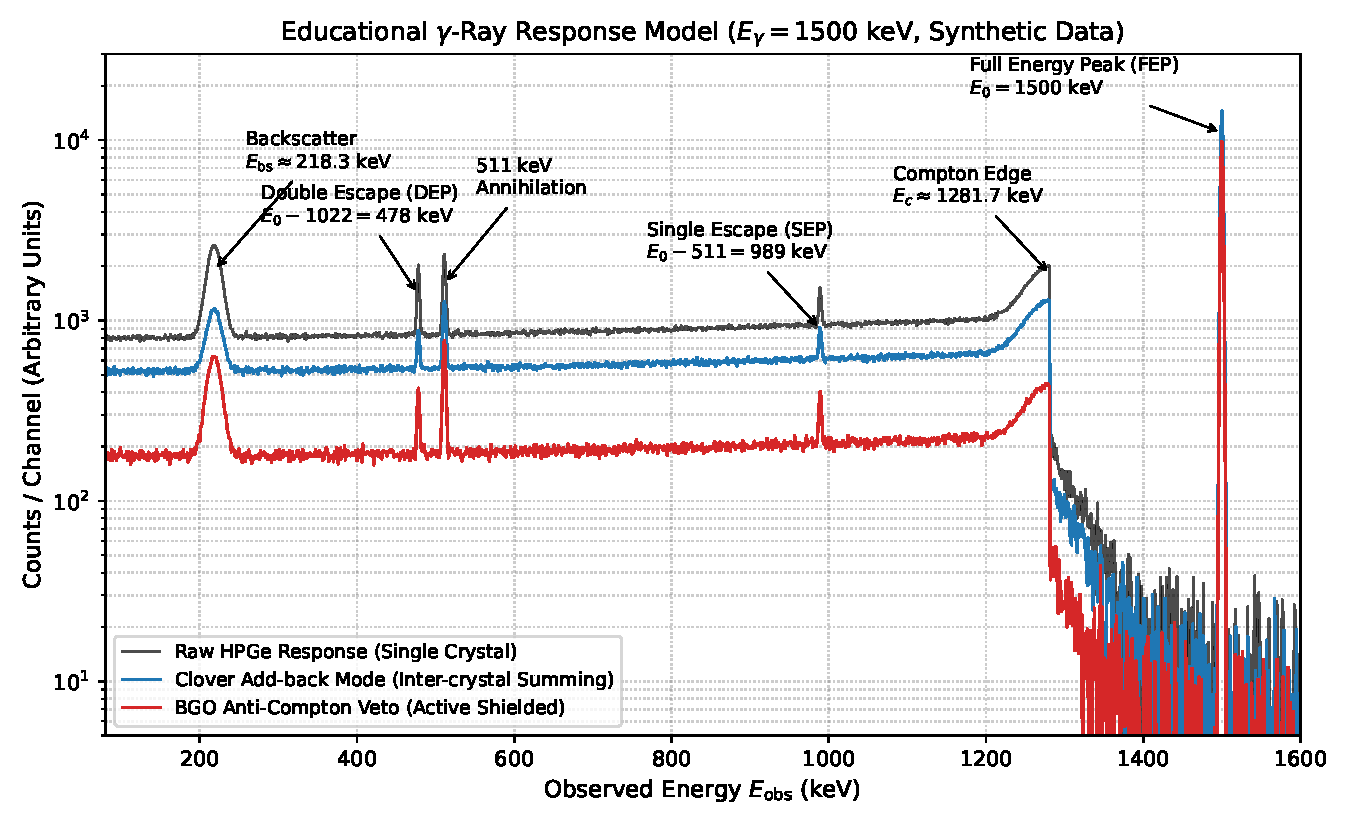
\includegraphics[width=0.88\textwidth]{Img/detector-response-simulation.pdf}%
\caption[理想 $\gamma$ 射线探测器响应谱模拟对比]{理想 $\gamma$ 射线探测器响应谱模拟对比（教学模型，基于参数化教学合成模型生成，明确区分晶体本征逃逸谱与靶室/屏蔽等周围材料引入的后向散射及湮灭吸收峰，入射能量取 $E_\gamma = 1500\,\text{keV}$。图中清晰标定了全能峰 FEP、$E_{\mathrm{edge}} \approx 1281.7\,\text{keV}$ 的康普顿边缘、单逃逸峰 SEP、双逃逸峰 DEP、$511\,\text{keV}$ 湮灭峰以及反向散射峰 $E_{\mathrm{bs}} \approx 218.3\,\text{keV}$。黑色实线代表单晶裸锗响应，蓝色曲线展示了 Clover 四晶体 Add-back 能量合并对全能峰的回收增强（图中展示的 Add-back 增益因子为选取的教学合成参数，非未知探测器实测值），红色曲线展示了 BGO 反康普顿屏蔽门控对连续本底与逃逸峰的主动抑制；注意此处为规范教学模型输出，纵轴为任意单位对数计数，非特定未知用户硬件实测拟合；各曲线未作单位面积归一，不作为条件概率密度的数值标定）。}
\label{fig:5-2-detector-response}
\end{figure}

\subsection{能量分辨率的微观物理贡献与独立性假定}\label{subsec:5-2-3}

探测器的能量分辨率表征其区分相近跃迁谱线的能力，通常以全能峰在半高全宽（Full Width at Half Maximum, FWHM）处的能量展宽 $\Delta E$ 表示。

HPGe 探测器的总能量分辨率由三类物理来源截然不同的涨落机制共同决定（吴治华教材第5章第三节印141/PDF149式(5.14)–(5.15)的载流子统计，以及第四节印146–151/PDF154–159的HPGe结构~\cite{book-wu-nuclear-experiment-methods}）：
\begin{enumerate}
\item 载流子产生的统计涨落（$\mathrm{FWHM}_{\mathrm{stat}}$）：
沉积能量 $E_\gamma$ 产生电子-空穴对的平均数目为 $N = E_\gamma / \epsilon$（吴治华教材印141/PDF149给出的77 K锗平均电离能为 $\epsilon \approx 2.96\,\text{eV}$）。由于部分能量耗散于不可逆的晶格声子激发，产生电子-空穴对数的涨落方差偏离纯泊松分布，由无量纲 Fano 因子 $F$ 修正（同页采用锗 $F=0.13$，并指出不同文献值存在差异；具体探测器应使用相应条件下的取值）：电子—空穴对数目的方差为无量纲数 $\sigma_N^2 = F N = F E_\gamma / \epsilon$。转换到观测能量尺度的等效能量方差为 $\sigma_{E, \mathrm{stat}}^2 = \epsilon^2 \sigma_N^2 = F \epsilon E_\gamma$（在 $\epsilon$ 与 $E_\gamma$ 均换成MeV时，单位为 $\mathrm{MeV}^2$），对应的半高全宽能量展宽为：
\begin{equation}\label{eq:5-2-fwhm-stat}
\mathrm{FWHM}_{\mathrm{stat}} = 2\sqrt{2\ln 2} \sigma_{E, \mathrm{stat}} = 2\sqrt{2\ln 2} \sqrt{F \epsilon E_\gamma} \approx 2.355 \sqrt{F \epsilon E_\gamma}.
\end{equation}
统计展宽随能量平方根 $\sqrt{E_\gamma}$ 增长，构成了半导体探测器物理分辨率的理论极限。
\item 电荷收集不完全与空间弥散（$\mathrm{FWHM}_{\mathrm{cc}}$）：
由于晶体内深能级杂质引起的载流子俘获（Trapping）、晶体缺陷导致的寿命缩短，以及不同电离位置的空穴漂移路径与收集时间起伏，产生电荷收集效率分散。此外，第~5.3~节讨论的弹道亏损（Ballistic Deficit）亦会展宽收集不完全项。该项近似正比于沉积能量 $E_\gamma$。
\item 电子学热噪声与基线晃动（$\mathrm{FWHM}_{\mathrm{el}}$）：
输入级的等效电压噪声、包括探测器反向漏电流在内的电流噪声，以及第~5.3~节式~\eqref{eq:5-3-var-net} 所述的基线滑动平均涨落 $\sigma_{BL}$。该项取决于读出电路、漏电流与基线估计等条件，与入射光子能量 $E_\gamma$ 基本无关。
\end{enumerate}

在各分量近似服从高斯分布或具有等效高斯二阶矩、且相互统计独立的假定下，总能量分辨率满足等效方差叠加律：
需要说明：不完全电荷收集项（$\mathrm{FWHM}_{\mathrm{cc}}$）通常引入低能侧指数拖尾，具有非对称非高斯特征；式~\eqref{eq:5-2-fwhm-quad} 属于等效二阶矩方差近似。
\begin{equation}\label{eq:5-2-fwhm-quad}
\mathrm{FWHM}_{\mathrm{tot}} = \sqrt{\mathrm{FWHM}_{\mathrm{stat}}^2 + \mathrm{FWHM}_{\mathrm{cc}}^2 + \mathrm{FWHM}_{\mathrm{el}}^2} = \sqrt{a + b E_\gamma + c E_\gamma^2}.
\end{equation}
必须强调：总分辨率是由电荷电离统计、晶体载流子输运与电子学模拟噪声共同主导的物理响应，绝不能依据 ADC 采样速率或数字量化位数单方面推断能量分辨率，亦不能脱离实测校准向未知探测器套用虚构性能指标。

\subsection{复合探测器、Add-back模式与符合相加效应}\label{subsec:5-2-4}

为了克服单晶 HPGe 探测器在兆电子伏以上能区光电吸收几率低下、且大体积单晶电荷收集时间过长的物理限制，核物理实验广泛采用了复合探测器结构，其中最典型的是四叶草型 Clover 探测器。在特定复合探测器设计（如典型的 Clover 探测器）中，常将 4 块相互独立读出但紧密排列的同轴高纯锗晶体（部分典型实现采用 $n$ 型同轴晶体）集成在同一个低温杜瓦内；不同阵列的具体晶体类型、电极分段与几何尺寸依研制规范而异，不应作单一普遍化假定。

对于一个入射光子，若其在某单一晶体内经单步光电效应完全沉积，由该晶体独立输出全能信号；若光子在晶体 A 发生初级康普顿散射，散射光子进入相邻的晶体 B 并在其中被完全光电吸收，在符合时间窗口 $\Delta T_{\mathrm{add}}$ 内，通过将两晶体的测得能量直接相加（$E_{\mathrm{add}} = E_A + E_B$），即可将原本属于康普顿本底的散射事件重新挽回为全能峰事件。这种数据重构机制称为 Add-back 模式。

在应用 Add-back 模式时，必须建立客观的得失权衡认知：
\begin{itemize}
\item 优势：显著增大了高能光子的全能峰绝对探测效率（回收程度取决于光子能量、晶体几何及接受条件），并有效提升了谱图的峰总比 $(P/T)$；
\item 代价：由于能量是由两路物理晶叶信号相加重构（$E_{\mathrm{add}} = E_A + E_B$），总能量方差不仅包含两晶叶的固有噪声，还受晶体间能量分配涨落与电子学相关的调控：$\sigma_{\mathrm{add}}^2 = \sigma_A^2 + \sigma_B^2 + 2\mathrm{Cov}(E_A, E_B)$。若两通道模拟前放电子学噪声相互独立，纯电子学噪声方差线性相加（$\sigma_{\mathrm{add, el}}^2 = \sigma_{A, \mathrm{el}}^2 + \sigma_{B, \mathrm{el}}^2$）；但在完整的物理能量求和中，实际能量分辨率还受晶体间能量分配起伏、接触层电容串扰协方差以及各晶叶电荷收集时间不一致性的影响，其总效应需按具体能量分配与噪声模型评价，不能普遍预设相对于单晶的展宽方向；此外，多道求和改变了事件的多重性分布，增大了探测偶然符合以及相邻晶体间的相加污染，并非所有谱学指标均无条件得到改善。
\end{itemize}

在紧凑阵列几何下，必须严格区分两类机制截然不同的脉冲相加现象：
\begin{enumerate}
\item 偶然堆积相加（Accidental Pile-up）：
源于不相干核反应事件发射的光子在极高计数率下由于时间重叠进入同一成形窗（见第~5.3~节与第~5.5~节）。该相加几率强烈正比于实验总计数率 $R_{\mathrm{tot}}$，通过降低束流强度或减小成形时间可以压制。
\item 真符合相加（True Coincidence Summing, TCS）：
发生在同核级联退激的微观过程中。当某激发能级相继发射符合光子 $\gamma_1$ 与 $\gamma_2$ 时，若两光子在收集时间窗口内同时击中同一个物理晶体（或处于同一 Clover 的不同晶叶），探测器直接记录其能量总和。在理想线性响应、固定立体角几何与无死时间阻塞的前提下，真符合相加的单事件相对发生概率严格与源的活度或宏观计数率无关（因为两光子源于同一次微观核退激），而是由初末态跃迁分支比、级联角关联函数 $W(\theta_{12})$ 以及探测器对源张开的绝对几何立体角 $\Omega$ 共同决定；但在实际高计数率在束反应中，宏观脉冲堆积与死时间门控会非线性改变观测到的相加损失与有效峰面积，导致观测到的相加修正呈现复杂的计数率依赖偏离：
\begin{itemize}
\item 相加滑出（Summing-Out）：本应归属于能量 $E_1$ 全能峰的事件，因伴随的 $\gamma_2$ 同时沉积能量而滑出 $E_1$ 峰位，导致 $E_1$ 处的表观峰面积减小：
\begin{equation}\label{eq:5-2-summing-out}
A_{\gamma 1}^{\mathrm{obs}} \approx A_{\gamma 1} \left[ 1 - \sum_j b_{1j} \varepsilon_{\mathrm{tot}}(E_j) \bar{W}_{1j} \right];
\end{equation}
式中 $b_{1j}$ 为已发出 $\gamma_1$ 条件下伴随 $\gamma_j$ 的光子发射概率，须包含级联分支和内转换对光子份额的影响，$\varepsilon_{\mathrm{tot}}$ 为伴随光子的总探测效率，$\bar{W}_{1j}$ 为包含探测器有限张角平均的级联角关联因子；该式为弱相加几率下的一阶近似，多级串联退激须结合衰变纲图进行完整矩阵积分以避免多重通道重复计数；
\item 相加滑入（Summing-In）：若两级联光子均在同一探测单元内发生完全能量沉积，在 $E_1 + E_2$ 处形成非本征跃迁的假复合相加峰。
\end{itemize}
\end{enumerate}
在紧凑的近距离靶--探测器几何下，真符合相加会显著改变表观峰面积。在反演分支比与跃迁几率时，不能简单假定各光子独立探测，必须通过已知放射源标定或数值模拟进行几何相关的相加修正。

\subsection{反康普顿屏蔽、极化灵敏度与径迹重构前沿}\label{subsec:5-2-5}

为了净化 HPGe 谱图并提取电磁辐射的内禀几何取向，现代 $\gamma$ 阵列引入了主动屏蔽与高级成像技术：
\begin{enumerate}
\item BGO 反康普顿主动屏蔽（Anti-Compton Veto）：
在 HPGe 晶体周围包裹高密度、高原子序数的锗酸铋（$\mathrm{Bi}_4\mathrm{Ge}_3\mathrm{O}_{12}$, BGO）闪烁体探测器（吴治华教材第10章第五节，印279/PDF287的反符合环讨论与图10.27~\cite{book-wu-nuclear-experiment-methods}）。当入射光子在 HPGe 内发生康普顿散射并将散射光子甩出晶体外时，逃逸光子极易被外围的 BGO 捕获并发光。通过将 HPGe 与 BGO 输出施加符合禁止门控（Veto Gate），系统自动舍弃发生逃逸的变形脉冲，可压低被该否决条件识别的康普顿连续谱及部分逃逸事件，改善峰总比；具体改善程度需由相应几何和阈值下的测量或输运计算确定。
需要说明：BGO 屏蔽无法做到完全消除本底，且伴随有假否决（False Veto）风险——从靶室散射的低能粒子、重离子核反应产生的快中子或散射本底、以及其它不相关级联光子若误入 BGO，会将合法的 HPGe 全能峰事件错误否决。因此，BGO 阈值与否决门宽必须精细标定。
\item Clover 康普顿散射偏振计（Compton Polarimeter）：
根据相对论量子电动力学 Klein-Nishina 微分截面，线偏振光子的康普顿散射强烈偏向于垂直于电矢量 $\mathbf{E}$ 的方位角平面（Hamilton 1975 专著第 15 章第 5 节，PDF 第 727–728 页，印刷第 716–717 页~\cite{book-hamilton-electromagnetic-interaction}）：
\begin{equation}\label{eq:5-2-klein-nishina-pol}
\frac{\mathrm{d}\sigma}{\mathrm{d}\Omega} = \frac{r_0^2}{2} \left(\frac{E'}{E}\right)^2 \left[ \frac{E'}{E} + \frac{E}{E'} - 2\sin^2\theta \cos^2\phi \right],
\end{equation}
其中 $\phi$ 为散射平面与电矢量偏振平面的夹角。在 Clover 探测器中，相互正交排列的 4 块晶体自然构成了康普顿散射计与吸收计。通过测定光子在平行于反应平面与垂直于反应平面内的散射计数不对称度：
\begin{equation}\label{eq:5-2-asymmetry}
A = \frac{N_\perp - a N_\parallel}{N_\perp + a N_\parallel} = Q P,
\end{equation}
其中 $Q$ 为偏振灵敏度因数，$P$ 为入射光子的线偏振度，参数 $a \equiv N_\perp^0 / N_\parallel^0$ 为利用无偏振放射源（$P=0$）标定的探测器几何不对称校正因子（与第~5.7~节式~\eqref{eq:5-7-asym-exp} 约定一致；若采用倒数定义则公式须相应变换）。通过偏振度 $P$ 的正负符号，可以实验判定特征 $\gamma$ 射线属于电性辐射还是磁性辐射（如鉴别 $E1$ 与 $M1$）。必须指出：偏振度符号与电磁性质的对应关系依赖于核态自旋跃迁序列与探测器几何放置角，不能采用“$P$ 为正必为电性辐射”的机械简化，具体极化反演将在第~5.7~节详细展开。
\item 现代 $\gamma$ 射线跟踪技术（$\gamma$-Ray Tracking, AGATA 与 GRETINA）~\cite{akkoyun-2012-agata-instrument-response}：
传统加装 BGO 屏蔽的阵列面临着几何立体角受限（大量的立体角被被动材料或大体积辅助闪烁体屏蔽体占据）的根本瓶颈。以 AGATA（欧洲）与 GRETINA（美国）为代表的新一代阵列采用了高纯锗晶体电极高度电分段技术（如单晶分段为 36 个独立电极），结合脉冲形状分析（Pulse Shape Analysis, PSA）技术，能够在离线或具备专用硬件流水线的系统中反演相互作用点的三维空间坐标 $(x, y, z)$ 与能量沉积（位置分辨可达毫米量级；Akkoyun 等 2012 手稿 arXiv:1111.5731v1 41页手稿 PDF 第 1–10 页概述了其总体架构与技术规范，区分于最终期刊排版页码）。
进而，基于康普顿散射运动学角守恒进行正向径迹重构（Forward Tracking），在算法层面识别单光子的散射径迹序列，从而摆脱了厚重 BGO 辅助屏蔽体的几何限制；新一代阵列设计以追求接近 $4\pi$ 的高立体角覆盖为目标（模拟中设想的完整 $4\pi$ 阵列由 180 块六角分段晶体组成，实际在束实验均按分阶段安装的子阵列如 AGATA Demonstrator 等构型运行，其覆盖立体角依安装几何与辅助探测器配置而异）。组合脉冲形状分析与径迹重构技术能够显著提升全能峰重建效率并压制康普顿散射本底，反映了在束核谱学探测技术的重要发展。
\end{enumerate}
%
}{%
    \section{探测器与光子响应 [未完成]}\label{sec:5-2}%
    \textit{本节尚未完成。}%
}

%-- Section 5.3: 数字成形与能量估计
\setcounter{section}{2}%
\IfFileExists{Tex/Sections/sec-5-3.tex}{%
    \section{数字成形与能量估计}\label{sec:5-3}

在低能核物理与在束 $\gamma$ 谱学实验中，探测器测得的特征 $\gamma$ 跃迁能量与谱峰面积，是确定核能级位置、跃迁多极性与绝对跃迁几率 $B(XL)$ 的实验输入。然而，本节以半导体探测器为例：能量沉积首先产生载流子，电荷运动与前置放大器将其转化为波形；闪烁探测器还包含光产生及光电转换等环节。传统的模拟核电子学通过电阻、电容与放大器构建模拟成形网络来获取脉冲幅度；而在现代数字化数据获取系统中，前置放大器输出信号由高速模数转换器（ADC）直接进行均匀离散时间采样，将连续波形转化为离散序列~\cite{wu-hongyi-2020-general-purpose-digital-daq-thesis, wu-2021-general-purpose-digital-daq-waveform-analysis}。

这一技术转换使得能量提取能够通过离散滤波算法在数字信号处理器或可编程逻辑门阵列（FPGA）中灵活实现。然而，数字成形并非简单执行数学平滑，其离散递推结构、极零消除匹配、平顶时间参数以及堆积判弃逻辑，直接决定了能谱的分辨率、峰位稳定性与有效计数率响应。若对算法环节的物理机制与响应边界缺乏清晰把握，测得的峰面积与强度比值便可能掺入仪器响应偏差。本节从探测器电荷积分波形出发，系统推导离散梯形滤波与极零消除递推算法，分析平顶成形对弹道亏损的缓解效果与物理边界，并讨论基线扰动及堆积判弃对核谱学能量与强度的系统性影响。

\subsection{探测器电荷收集与前放信号的物理生成}\label{subsec:5-3-1}

半导体探测器记录 $\gamma$ 射线的初始物理过程是带电次级粒子在晶体中的电离能量损失。当入射能量为 $E_\gamma$ 的光子在晶体内完全沉积其能量时，在理想完整收集条件下，单个读出电极所对应的收集电荷绝对值可写为：
\begin{equation}\label{eq:5-3-q0}
Q_0 = \frac{e E_\gamma}{\epsilon},
\end{equation}
其中 $e$ 为元电荷，$\epsilon$ 为探测介质中平均产生一对电子-空穴对所需的电离能量。关于具体探测器的电荷输运与探测物理，将在第~5.2~节展开讨论。

在工作电场下，电子和空穴漂移并在读出电极上诱导电流。相互作用位置、漂移路径与收集过程的差异，使脉冲前沿具有有限且变化的持续时间。具体输运与电极响应留在第~5.2~节；这里关心这种前沿差异怎样进入数字能量估计。

感应电荷随后进入电荷灵敏前置放大器（CSPA）。前置放大器利用反馈积分电容 $C_f$ 积分输入电流，并在输出端产生阶跃电压脉冲；同时，并联的反馈电阻 $R_f$ 提供直流泄放通道，使电荷缓慢释放，形成长指数衰减尾部。考虑载流子收集过程引入的有效上升时间参数 $\tau_r$ 与前放反馈衰减时间常数 $\tau_d = R_f C_f$，前放输出的模拟电压脉冲可唯象描述为：
\begin{equation}\label{eq:5-3-vt}
v(t) = \frac{Q_0}{C_f} \left(1 - e^{-t/\tau_r}\right) e^{-t/\tau_d} \, u(t),
\end{equation}
其中 $u(t)$ 为连续时间单位阶跃函数。为了抑制前放反馈电阻带来的并联热电流噪声，通常需要选取阻值很大的反馈电阻，这使得衰减时间常数 $\tau_d$ 显著长于脉冲上升沿。在在束核物理实验中，当事件计数率较高时，相继到达的脉冲往往叠加在先前脉冲尚未完全衰减的长尾上，产生尾部堆积。

高速模数转换器以均匀采样周期 $T_s$ 对连续电压波形 $v(t)$ 进行离散采样，生成离散时间数据序列：
\begin{equation}\label{eq:5-3-vn}
v[n] = v(n T_s), \quad n = 0, 1, 2, \dots
\end{equation}
数字能量滤波算法的目标，便是在离散时间域内设计线性时不变（LTI）算子，消除前置放大器的指数衰减长尾，平抑电荷收集时间涨落对幅度测量的影响，并在白噪声存在下提取出正比于沉积能量 $E_\gamma$ 的脉冲高度。

\subsection{离散梯形滤波与极零消除的递推实现}\label{subsec:5-3-2}

梯形滤波器通过有限长度的差分和累加构造平坦顶部，便于在一段时间窗内提取幅度，并协调噪声、脉冲宽度与收集时间变化。它的适用性取决于输入响应和噪声条件，不能只凭某个滤波器名称认定其对全部波形最优~\cite{wu-hongyi-2020-general-purpose-digital-daq-thesis, wu-2021-general-purpose-digital-daq-waveform-analysis}。

基于差分与累加的离散递推梯形滤波算法可表述如下：设采样周期为 $T_s$，滤波器的上升时间采样点数为 $k$，平顶终止延迟采样点数为 $\ell$，并满足结构约束 $\ell \ge k$。成形后的梯形脉冲具有对称的上升时间 $k T_s$、平顶宽度 $(\ell - k) T_s$ 以及基底总宽度 $(k + \ell) T_s$。极零消除（PZC）由离散时域匹配参数 $M$ 引入：
\begin{equation}\label{eq:5-3-m-pzc}
M = \frac{1}{e^{T_s / \tau_d} - 1}.
\end{equation}
在 $T_s \ll \tau_d$ 条件下，一阶近似给出 $M \approx \tau_d / T_s$。但在离散递推算法中，采用严格的指数定义式才能确保时域极点完全相消。

在零初始历史（$n < 0$ 时 $v[n] = 0$）的假设下，递推梯形滤波由四延迟差分、一级累加、极零加权与二级累加构成：
\begin{align}
d[n] &= v[n] - v[n-k] - v[n-\ell] + v[n-k-\ell], \label{eq:5-3-dn} \\
p[n] &= p[n-1] + d[n], \label{eq:5-3-pn} \\
r[n] &= p[n] + M d[n], \label{eq:5-3-rn} \\
s[n] &= s[n-1] + r[n]. \label{eq:5-3-sn}
\end{align}
此处对文献符号作明确说明：吴鸿毅学位论文~\cite[第~20~页，式~(1.14)、(1.19)]{wu-hongyi-2020-general-purpose-digital-daq-thesis}末项印为 $n[n-k-\ell]$，在符号上与样本时间索引 $n$ 存在歧义；为保证递推滤波器的线性时不变（LTI）结构与物理因果律，本任务在数学推导中将其重建为第四个输入采样延迟项 $v[n-k-\ell]$。此处保留原文符号记录并明确任务重建依据，未核对作者勘误前不对原稿排印原因作先验断定。

为分析该递推系统的频率响应与极点相消机制，对其进行 $z$ 变换。设 $v[n-m] \leftrightarrow z^{-m} V(z)$，差分序列 $d[n]$ 的变换为：
\begin{equation}\label{eq:5-3-dz}
D(z) = \left(1 - z^{-k}\right) \left(1 - z^{-\ell}\right) V(z).
\end{equation}
累加操作对应离散积分因子 $(1 - z^{-1})^{-1}$，经极零加权后，中间序列 $r[n]$ 的 $z$ 变换为：
\begin{equation}\label{eq:5-3-rz}
R(z) = \left(\frac{1}{1 - z^{-1}} + M\right) D(z) = \frac{(M+1) - M z^{-1}}{1 - z^{-1}} D(z).
\end{equation}
经过第二级累加，输出序列 $s[n]$ 的系统传递函数 $H(z) = S(z) / V(z)$ 表达为：
\begin{equation}\label{eq:5-3-hz}
H(z) = \frac{(M+1) - M z^{-1}}{(1 - z^{-1})^2} \left(1 - z^{-k}\right) \left(1 - z^{-\ell}\right).
\end{equation}
利用长度为 $k$ 与 $\ell$ 的滑动矩形求和序列（boxcar）的 $z$ 变换恒等式：
\begin{equation}\label{eq:5-3-boxcar}
B_k(z) = \sum_{m=0}^{k-1} z^{-m} = \frac{1 - z^{-k}}{1 - z^{-1}}, \quad B_\ell(z) = \sum_{j=0}^{\ell-1} z^{-j} = \frac{1 - z^{-\ell}}{1 - z^{-1}},
\end{equation}
系统传递函数可重写为：
\begin{equation}\label{eq:5-3-hz-boxcar}
H(z) = \left[(M+1) - M z^{-1}\right] B_k(z) B_\ell(z).
\end{equation}

考察输入为理想单指数衰减阶跃脉冲 $v[n] = A \alpha^n u[n]$，其中幅度为 $A$，离散极点为 $\alpha = e^{-T_s / \tau_d}$。由 $M$ 的定义可知：
\begin{equation}\label{eq:5-3-alpha-m}
M = \frac{\alpha}{1 - \alpha} \implies \alpha = \frac{M}{M + 1}.
\end{equation}
输入信号的 $z$ 变换为：
\begin{equation}\label{eq:5-3-vz}
V(z) = \frac{A}{1 - \alpha z^{-1}} = \frac{A (M+1)}{(M+1) - M z^{-1}}.
\end{equation}
将 $V(z)$ 代入系统输出表达式：
\begin{align}\label{eq:5-3-sz}
S(z) &= H(z) V(z) \nonumber \\
     &= \left[(M+1) - M z^{-1}\right] B_k(z) B_\ell(z) \cdot \frac{A (M+1)}{(M+1) - M z^{-1}} \nonumber \\
     &= A (M+1) B_k(z) B_\ell(z).
\end{align}
分子项 $(M+1) - M z^{-1}$ 与输入极点因式严格对消。在时域中，输出序列 $s[n]$ 等价于两个分别具有 $k$ 与 $\ell$ 个单位抽头的矩形序列的离散卷积乘上常数 $A (M+1)$。

在 $\ell \ge k$ 条件下，两矩形序列的卷积在区间 $k - 1 \le n \le \ell - 1$ 内达到最大重叠和 $k$。因此，对于幅度为 $A$ 的纯指数输入，梯形输出在平顶区间的严格高度为：
\begin{equation}\label{eq:5-3-sflat}
s_{\text{flat}} = A k (M + 1).
\end{equation}
根据上述解析推导，为从平顶高度 $s_{\text{flat}}$ 提取输入阶跃幅度 $A$，归一化除数应取 $k (M + 1)$，即归一化成形序列定义为：
\begin{equation}\label{eq:5-3-snorm}
s_{\mathrm{norm}}[n] = \frac{s[n]}{k (M + 1)}.
\end{equation}
若直接取 $k M$，将引入大小为 $(M+1)/M = e^{T_s / \tau_d}$ 的系统性增益偏置。增益相对偏置为：
\begin{equation}\label{eq:5-3-gain-bias}
\frac{M+1}{M} - 1 = e^{T_s/\tau_d} - 1.
\end{equation}
在后续讨论采用的教学模型参数（$T_s = 10\text{ ns}$，$\tau_d = 50\ \mu\text{s}$，对应 $T_s / \tau_d = 2 \times 10^{-4}$）下，该相对偏置约为 $0.0200\%$。这是由离散差分结构确定的数值增益控制，用以保证算法在理想条件下的无偏响应。

\subsection{弹道亏损、平顶宽度与能量估计的物理边界}\label{subsec:5-3-3}

上述极点相消假定了瞬时电荷收集（$\tau_r = 0$）。在实际探测器中，有限载流子收集时间使脉冲具有有限上升沿。若采用零平顶的三角形滤波器（$\ell = k$），滤波器在单一极值点取样。当晶体内部相互作用深度或漂移路径导致有效上升时间延长时，脉冲上升过程尚未完全结束便已受到成形滤波器的下削作用，使得输出峰值幅度低于瞬时电荷收集情形下的理论高度。这种由电荷收集过程的时间尺度与涨落引起的脉冲峰值损失，即为弹道亏损（ballistic deficit）。

弹道亏损在能谱中不仅造成峰位整体向低能侧偏移，而且由于同一单能光子在探测器不同位置电离时产生的脉冲上升时间各不相同，幅度亏损的统计展宽会导致全能峰向低能方向产生非对称拖尾，显著恶化能量分辨率。

设置平顶区间（$\ell > k$）的主要目的即在于平抑弹道亏损。当平顶宽度 $T_{\text{flat}} = (\ell - k) T_s$ 覆盖了主要的电荷收集区间时，输出波形能够在一段采样窗口内保持相对平缓的顶部平台，从而降低幅度提取对前沿细节的敏感度。

然而，在物理讨论中不能断言“平顶宽度超过名义收集时间当且仅当完全消除弹道亏损”。这一局限性体现在以下方面：

第一，前放输出的前沿波形通常由多级弛豫过程决定，在连续模型中常用双指数前沿 $A (1 - e^{-t/\tau_r}) e^{-t/\tau_d}$ 唯象描述。参数 $\tau_r$ 反映的是前沿演化的特征弛豫时间，输入信号渐近趋近峰值，并不存在一个使电流严格突变为零的时域硬边界。

为定量考察这一特征，表~\ref{tab:5-3-ballistic-deficit} 汇总了基于规范双指数脉冲模型在无噪声条件下的数值计算结果。计算参数采用采样周期 $T_s = 10\text{ ns}$、衰减常数 $\tau_d = 50\ \mu\text{s}$、上升成形参数 $k = 200$（对应成形时间 $2.0\ \mu\text{s}$），并在不同平顶参数下扫描前沿上升参数 $\tau_r$（$20$–$400\text{ ns}$）。输出先按式~\eqref{eq:5-3-snorm} 增益归一为 $s_{\mathrm{norm}}[n]=s[n]/[k(M+1)]$，再取 $\widehat A=\max_n s_{\mathrm{norm}}[n]$。输入幅度为 $1000$ 任意单位，亏损百分比定义为 $100\% \times (1000-\widehat A)/1000$；这不是能量刻度后的实测分辨率。模型参数、数据与程序见附录~F。

\begin{table}[!htbp]
\centering
\caption[不同前沿上升参数 $\tau_r$ 与平顶宽度下的弹道亏损数值计算对比]{不同前沿上升参数 $\tau_r$ 与平顶宽度下的弹道亏损数值计算对比（计算基于附录~F 规范双指数脉冲模型在无噪声条件下的模拟数据，取 $T_s = 10\text{ ns}$、$\tau_d = 50\ \mu\text{s}$、成形参数 $k = 200$，输入幅度 $A = 1000$ 任意单位；输出序列首先按式~\eqref{eq:5-3-snorm} 归一化为 $s_{\mathrm{norm}}[n] = s[n]/[k(M+1)]$ 后取极大值 $\widehat{A} = \max_n s_{\mathrm{norm}}[n]$，弹道亏损定义为 $100\% \times (1000 - \widehat{A})/1000$。数据严格来自 \texttt{ballistic\_deficit\_study.csv}，未包含探测器实际空间电荷收集分布与连续电子学噪声）。}
\label{tab:5-3-ballistic-deficit}
\begin{tabular}{cccc}
\toprule
上升参数 $\tau_r$ & 零平顶 ($0\text{ ns}$) & 短平顶 ($100\text{ ns}$) & 宽平顶 ($400\text{ ns}$) \\
(ns) & 亏损 $\Delta E / E$ & 亏损 $\Delta E / E$ & 亏损 $\Delta E / E$ \\
\midrule
20  & 0.7144\%  & 0.0560\%  & 0.0508\% \\
60  & 2.1990\%  & 0.6455\%  & 0.1336\% \\
100 & 3.6594\%  & 1.7643\%  & 0.2958\% \\
140 & 5.1099\%  & 3.0538\%  & 0.6718\% \\
180 & 6.5583\%  & 4.4123\%  & 1.2791\% \\
220 & 8.0030\%  & 5.7955\%  & 2.0735\% \\
300 & 10.8680\% & 8.5933\%  & 4.0447\% \\
400 & 14.3807\% & 12.0648\% & 6.8916\% \\
\bottomrule
\end{tabular}
\end{table}

\begin{figure}[!htbp]
\centering
%
  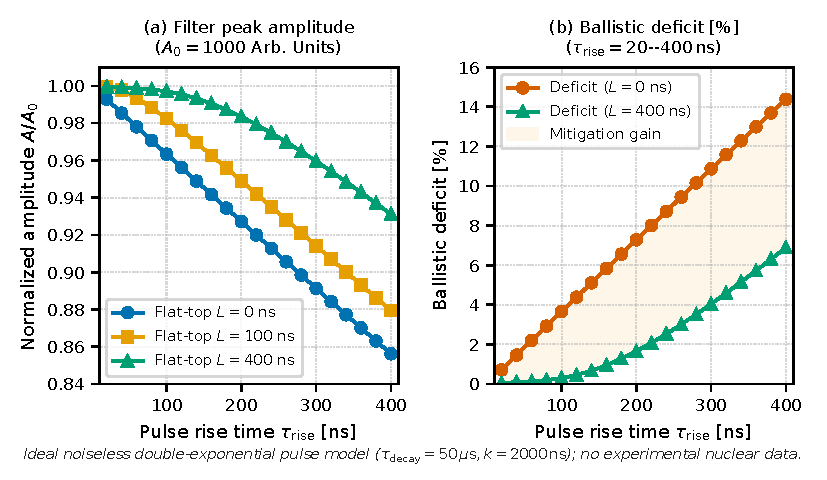
\includegraphics[width=0.85\textwidth]{Img/digital-energy-response.pdf}%
\caption[理想双指数输入下数字梯形滤波响应与弹道亏损缓解特征]{理想双指数输入下数字梯形滤波响应与弹道亏损缓解特征（教学模型，基于附录~F 与 \texttt{ballistic\_deficit\_study.csv} 规范生成，计算参数取 $T_s = 10\text{ ns}$、$\tau_d = 50\ \mu\text{s}$、$\tau_r = 100\text{ ns}$、成形参数 $k = 200$。该曲线展示了不同平顶参数对前沿收集弛豫的平抑效果；注意此处为确定性数值模型输出，未包含探测器连续噪声、电荷收集时间空间非均匀分布及硬件量化限制）。}
\label{fig:5-3-digital-energy-response}
\end{figure}

表~\ref{tab:5-3-ballistic-deficit} 数据表明：延长平顶能够显著压缩不同上升时间引起的幅度差异（例如在 $\tau_r = 220\text{ ns}$ 时，亏损由 $0\text{ ns}$ 平顶的 $8.0030\%$ 降至 $400\text{ ns}$ 平顶的 $2.0735\%$）。但在给定渐近双指数输入与离散取幅规则的本模型中，即使平顶达到 $400\text{ ns}$，依然保留有确定的残余亏损。

第二，极零匹配对平顶形态具有决定性影响。若滤波参数 $M$ 与物理脉冲的衰减时间 $\tau_d$ 存在偏差，平顶区域可能出现斜率或弯曲，不能再按理想平台取幅。此时在名义平顶区间内取幅，测量结果将直接受取样时刻与脉冲到达相位的制约，重新引入测量分散性。

第三，滤波成形参数的选取受到噪声与通过率的双重制约。展宽平顶增加了滤波器的等效积分时间，将增大低频并联噪声在能量提取中的贡献。此外，基底总宽度 $(k + \ell) T_s$ 增加，使后发事件掉入成形时间窗内的概率升高。因此，平顶参数的确定是在弹道亏损平抑、高频与低频噪声折衷以及计数率能力之间寻求的平衡，而非单纯追求单项指标的极限。

\subsection{基线涨落、堆积判弃与核谱强度畸变机制}\label{subsec:5-3-4}

在核反应在束实验环境中，除了孤立脉冲的波形响应外，基线波动、极零失配与事件堆积构成了影响能量估计与能谱强度的关键仪器因素。

前置放大器输出波形通常叠加在一个包含慢漂移的基线上，其来源包括探测器漏电流随环境温度的变化、供电噪声以及远端未分辨脉冲的残留尾部。常用的基线校准方式是在触发脉冲到达之前，利用包含 $N$ 个采样点的无信号区间计算滑动均值~\cite{wu-hongyi-2020-general-purpose-digital-daq-thesis}：
\begin{equation}\label{eq:5-3-bl}
BL = \frac{1}{N} \sum_{m=1}^N v[n_{\text{trig}} - m],
\end{equation}
并在幅度提取时予以扣除。当离散基线采样点满足独立同分布的白噪声假设时，基线估计量的统计方差为 $\sigma_{BL}^2 = \sigma_v^2 / N$。在更一般的实际情形中，滤波与低频漂移会导致采样点之间存在自相关。从成形峰值 $s$ 中减去映射至相同增益刻度的基线估计 $BL$ 后，净幅度的方差满足：
\begin{equation}\label{eq:5-3-var-net}
\mathrm{Var}(s - BL) = \mathrm{Var}(s) + \mathrm{Var}(BL) - 2\mathrm{Cov}(s, BL).
\end{equation}
仅当成形峰值与基线估计相互统计独立且单位映射一致时，总方差才简化为两者的简单平方和。在大事件到达率下，缩短平均窗口 $N$ 会增大基线方差，进而展宽能量分辨率；但若盲目增大 $N$，基线窗极易跨入先前脉冲的衰减尾部，导致基线值被系统性抬高。

极零失配还会留下脉冲后的残差。在本递推与给定指数输入下，采用大于真实匹配值的 $M$ 会产生负残差，反向失配则可留正尾。后续事件可能叠加其上，但最终取幅偏差还取决于基线追踪、扣除、时间位置与判弃逻辑。因此，残差形状和计数率依赖性可用于检验仪器解释，不能直接把某一种残差与所有实现中的固定方向能量偏移对应起来。

为了处理脉冲重叠，数字系统通常采用快慢双滤波通道结构~\cite{wu-hongyi-2020-general-purpose-digital-daq-thesis, wu-2021-general-purpose-digital-daq-waveform-analysis}：
\begin{enumerate}
\item 快通道（触发通道）：采用较短的微分成形参数（成形时间常在百纳秒量级），用于灵敏辨识脉冲前沿并标记事件到达时间。
\item 慢通道（能量通道）：采用成形时间在数微秒量级的精细梯形滤波器，用于滤除噪声并提取脉冲幅度。
\end{enumerate}
在声明的教学实现中，堆积判弃逻辑（PUR）通过快通道的时间标记监测慢通道的成形区间。若在慢通道的特征时间窗内（例如本模型中考查的基底窗口 $(k + \ell) T_s$）检测到第二个脉冲到达，系统将把该事件标记为堆积并予以剔除。在实际硬件固件中，否决窗口的具体形态与逻辑判定取决于具体的探测器与在线配置，并不普遍固定为单一形式。

堆积判弃在滤除变形脉冲、净化全能峰的同时，改变了核谱学的有效计数与事件接受几率。首先，堆积事件被剔除引入了非线性计数损失。对于平均事件率为 $R$ 的泊松过程，时间窗 $\Delta t$ 内至少发生一次后续到达的概率为：
\begin{equation}\label{eq:5-3-pur-poisson}
P(\ge 1; \Delta t) = 1 - e^{-R \Delta t},
\end{equation}
仅在 $R \Delta t \ll 1$ 的低计数率极限下近似表现为正比于窗口长度的线性响应。在在束实验中，当阵列不同角度位置的探测器承受不同计数率时，各通道的事件接受度产生相对差异。若未对各角度通道的有效活时间进行精细校正，将对角分布系数 $W(\theta)$ 与方向角关联（DCO）比值带来测量偏差。其次，在级联跃迁中，若同核相继发射的两个 $\gamma$ 光子在收集时间窗口内同时被同一个晶体吸收（真符合相加），脉冲在物理上直接叠加，当二者无法被单独分辨且均完全沉积能量时，幅度可对应能量和 $E_{\gamma 1}+E_{\gamma 2}$。部分沉积也会改变连续本底与峰计数。真符合相加可造成特定峰的求和损失或其它能量处的求和增加，分支提取须配套相应响应修正。

快触发通道提供的时间标记构成了在束实验符合判定的起点，而亚采样周期定时可采用过零插值恒比定时（CFD）等方法，其在不同信号幅度与采样相位下的时间走动将在第~5.4~节详细推导；而多探测器并发触发、数据缓存区满以及多通道联合活时间损失的定量修正，将在第~5.5~节进行系统分析。
%
}{%
    \section{数字成形与能量估计 [未完成]}\label{sec:5-3}%
    \textit{本节尚未完成。}%
}

%-- Section 5.4: 数字定时、同步与CFD
\setcounter{section}{3}%
\IfFileExists{Tex/Sections/sec-5-4.tex}{%
    \section{数字定时、同步与CFD}\label{sec:5-4}

能量标记说明一个脉冲沉积了多少能量，时间标记则用于判断不同探测器的信号是否属于同一次退激过程。第~5.3~节的慢成形适合估计幅度；时间提取更关心前沿、局部斜率和采样位置。吴鸿毅论文介绍的前沿甄别与恒比定时，以及 Lipschutz 等人的波形处理研究，提供了从采样点建立时间估计的具体路径~\cite{wu-hongyi-2020-general-purpose-digital-daq-thesis, doctoral-r1-g32-lipschutz-2016-pixie16-ddas-timing}。

首先要区分编码粒度、采样周期、插值误差、噪声抖动与实测时间分辨。设一个粗计数周期为 $T_{\mathrm{tick}}$，仅在其内部采用 $b$ 个有效细位作均匀分数编码时，数值步长才为：
\begin{equation}\label{eq:5-4-code-step}
\delta t_{\mathrm{code}} = \frac{T_{\mathrm{tick}}}{2^b};
\end{equation}
$b$ 无量纲，其余各量均为时间。这是教学编码关系，实际字中的状态位和模块映射另见第~5.5~节及附录~E。粗计数周期也不必等于 ADC 采样周期 $T_s$。插值可报告小于 $T_s$ 的时间间隔，但重复测量的散布仍受信号、算法与时钟影响，增加存储位数不会自动缩窄时间谱。

采样周期规定观察波形的时间网格，插值则利用相邻幅度中包含的前沿信息估计网格之间的位置；它没有新增一次独立的电压测量。插值误差描述估计相对给定参考的偏离，噪声抖动描述重复测量的随机变化，实际时间谱还可能包含探测器响应和漂移。因此，报告时间性能时应同时说明输入、估计算法、参考与宽度定义。

\subsection{恒比算子、参数约定与残余走动}\label{subsec:5-4-1}

固定阈值的前沿甄别记录信号首次越阈的时刻。在相同上升形状下，大幅度脉冲通常较早越阈，因而测得时间随幅度变化。恒比定时（constant fraction discrimination，CFD）通过延迟与比例相减寻找过零点，试图降低这种时间走动（time walk）。

沿用本任务模型，令 $F[n]$ 为快滤波输出，$n$ 为采样索引，$d$ 为正整数延迟样本数，$0<f<1$ 为无量纲分数，定义：
\begin{equation}\label{eq:5-4-cn}
C[n] = F[n-d] - f F[n].
\end{equation}
$F$ 与 $C$ 具有相同的幅度单位，实际延迟为 $d T_s$。本文模型选择脉冲到达后第一个由负至非负的过零区间。若其相邻样本满足 $C[n]<0\le C[n+1]$，且 $t_n=n T_s$，两点连线的零截距为：
\begin{equation}\label{eq:5-4-linear-zc}
\widehat{t}_{\mathrm{zc}} = t_n - \frac{C[n]}{C[n+1]-C[n]} T_s.
\end{equation}
该式给出插值估计；分母须非零，并须排除基线或噪声产生的无关穿越。吴鸿毅学位论文~\cite[第~25~页，式~(1.22)]{wu-hongyi-2020-general-purpose-digital-daq-thesis}采用 $x[n]-a x[n-k]$。Lipschutz 等人~\cite[式~(3)]{doctoral-r1-g32-lipschutz-2016-pixie16-ddas-timing}令 $n=i+D$ 后则为 $\mathrm{FF}[n]-w\mathrm{FF}[n-D]$。为比较记号，假设各式输入均为同一 $F$，并令原式的 $k=D=d$，则：
\begin{equation}\label{eq:5-4-cfd-map}
Y_a[n] = F[n] - a F[n-d], \qquad C[n] = -f Y_{1/f}[n].
\end{equation}
可见，同零点需要 $a=1/f$，Lipschutz 形式同理需要 $w=1/f$，并另乘整体因子 $-f$。原文方案不能只翻转符号、保留相同分数就与本文算子等同。本文模型采用上升穿越；其它实现的过零分支须随其波形极性、参数与选根条件分别说明~\cite{wu-hongyi-2020-general-purpose-digital-daq-thesis, doctoral-r1-g32-lipschutz-2016-pixie16-ddas-timing}。

例如 Lipschutz 分路测试的优化线性参数为 $(T_r, T_g, D, w)=(6, 2, 4, 5/8)$，优化三次参数为 $(2, 0, 4, 1/8)$。前三项是样本数，对应该实验 $4\,\mathrm{ns}$ 采样周期，$w$ 无量纲；$T_r$ 和 $T_g$ 分别控制快滤波的求和长度与间隙。这些小于 1 的 $w$ 不是本文 $f$ 的倒数，因此各方案需分别选取和校准定时点。

快滤波参数也参与定时：它们改变过零附近的曲率、斜率及噪声相关性。仅更换恒比分数、保留滤波参数，并不保证仍选中了适合原波形的定时区域。比较两种算法时，应区分算子、参数优化与插值方式各自的作用。

幅度不变性仍可在各自固定算子内成立。对同形、同到达相位的 $F[n]=A g[n]$，$A>0$，$g$ 为单位形状，有 $C[n]=A C_g[n]$，故：
\begin{equation}\label{eq:5-4-amp-inv}
\widehat{t}_{\mathrm{zc}} = t_n - \frac{A C_g[n]}{A [C_g[n+1]-C_g[n]]} T_s = t_n - \frac{C_g[n]}{C_g[n+1]-C_g[n]} T_s.
\end{equation}
这要求线性处理、无噪声且选中的过零分支不变，并不保证不同算子给出同一时间戳。真实前沿形状、基线偏移、饱和或采样相位变化会留下偏差；平均时间随能量的变化与随机展宽也须分别考察。局部小噪声近似下，若无噪声 CFD 曲线 $\bar{C}(t)$ 在过零 $t_\times$ 处斜率固定且非零，时间抖动可估为：
\begin{equation}\label{eq:5-4-timing-jitter}
\sigma_t \simeq \frac{\sigma_C}{|\bar{C}'(t_\times)|}.
\end{equation}
这里 $\sigma_C$ 是过零附近经过快滤波、延迟相减及相关性传播后的有效幅度噪声标准差，不能直接以原始 ADC 样本噪声替代。实际走动的方向和能量依赖应由标定确定；CFD 也不是唯一途径，前沿插值或波形函数拟合可按信号条件选用。

\subsection{采样相位与插值的条件比较}\label{subsec:5-4-2}

事件到达时刻 $t_0$ 相对本地采样网格的相位可写为 $\phi = t_0 \bmod T_s$，其中 $0 \le \phi < T_s$。过零附近曲线若有曲率，连接两个样本的直线通常不经过连续曲线的真实零点，误差便随 $\phi$ 变化。吴鸿毅学位论文~\cite[第~92--96~页]{wu-hongyi-2020-general-purpose-digital-daq-thesis}的模拟与分路测试显示了这种相位依赖；其中关于上升沿与采样周期的经验比较属于所用信号和算法，不能推广为统一分界。

表~\ref{tab:5-4-sampling-convergence} 沿用本任务的无噪声教学模型。输入波形在 $t \ge t_0$ 时取为：
\begin{equation}\label{eq:5-4-input-pulse}
v(t) = A \left[1 - e^{-(t-t_0)/\tau_r}\right] e^{-(t-t_0)/\tau_d},
\end{equation}
此前为零；$A = 1000$ 为任意幅度单位，$\tau_r = 100\,\mathrm{ns}$，$\tau_d = 50\,\mu\mathrm{s}$，$t_0 = 500\,\mathrm{ns} + \phi$。快滤波取两个长度为 $L$、间隔为 $G$ 的矩形求和之差再除以 $L$，其中 $L T_s = 100\,\mathrm{ns}$、$G T_s = 50\,\mathrm{ns}$；CFD 采用 $d T_s = 80\,\mathrm{ns}$ 和 $f = 0.4$，随后按前述上升过零规则插值，不作峰值取幅。

每个 $T_s$ 分别把其自身的有限延迟求和算子延拓到连续时间，再数值求该算子的上升过零根，得到参考延迟 $t_{\mathrm{ref}}$。比较的是 $\widehat{t}_{\mathrm{zc}} - (t_0 + t_{\mathrm{ref}})$。每行只扫描 $\phi/T_s = 0, 0.05, \dots, 0.95$ 这 20 个相位点；表值由既有 CSV 逐行读取，输入、程序和文件哈希见本节证据台账及附录~F。

\begin{table}[!htbp]
\centering
\caption{不同采样周期 $T_s$ 下 CFD 线性过零插值的采样相位误差收敛性对比（数据源自规范教学模型与 \texttt{sampling\_convergence.csv}，输入取 $A=1000$ 任意单位、$\tau_r = 100\text{ ns}$、$\tau_d = 50\ \mu\text{s}$、到达时刻 $t_0 = 500\text{ ns} + \phi$；快滤波参数取 $L T_s = 100\text{ ns}$、$G T_s = 50\text{ ns}$，CFD 延迟 $d T_s = 80\text{ ns}$、$f = 0.4$。参考延迟 $t_{\text{ref}}$ 由各采样周期下有限抽头算子延拓至连续时间的真实过零根确定。表中最大绝对误差仅覆盖离散采样的 20 个等间距相位点 $\phi/T_s \in \{0, 0.05, \dots, 0.95\}$，非连续全相位区间的解析全局上界；且计算在理想无噪声条件下进行，不包含真实探测器上升沿起伏、前放热噪声及电子学时钟抖动）。}
\label{tab:5-4-sampling-convergence}
\begin{tabular}{cccc}
\toprule
采样周期 $T_s$ & 采样率 & 参考延迟 $t_{\text{ref}}$ & 最大绝对误差 \\
(ns) & (MSPS) & (ns) & (ns，所采 20 相位点) \\
\midrule
10   & 100 & 157.1223 & 0.2566 \\
5    & 200 & 159.6536 & 0.1297 \\
2.5  & 400 & 160.8446 & 0.0137 \\
1.25 & 800 & 161.4716 & 0.0060 \\
\bottomrule
\end{tabular}
\end{table}

\begin{figure}[!htbp]
\centering
\IfFileExists{Img/cfd-phase-convergence.pdf}{%
  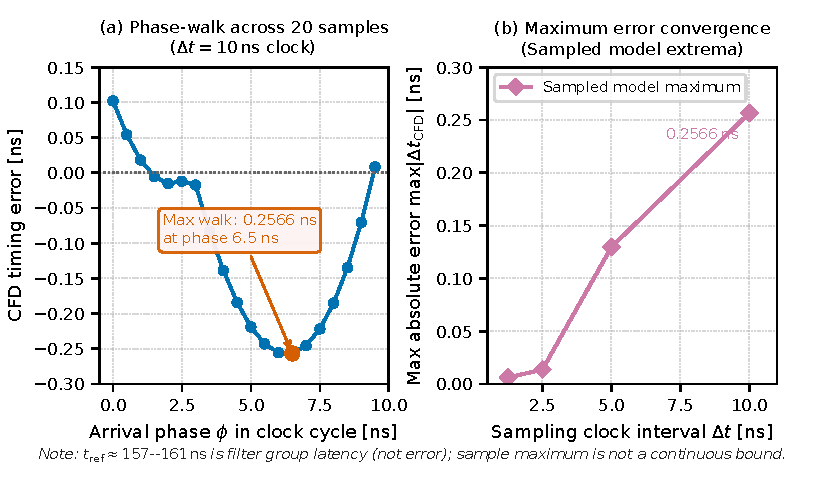
\includegraphics[width=0.85\textwidth]{Img/cfd-phase-convergence.pdf}%
}{%
  \fbox{\parbox{0.85\textwidth}{\centering\vspace{2cm}（图 5.2 待 G80 注入：\texttt{Img/cfd-phase-convergence.pdf}；展示不同采样周期下 CFD 过零插值误差随到达相位 $\phi/T_s$ 的演化曲线）\vspace{2cm}}}%
}
\caption{数字 CFD 过零插值误差随采样相位变化的收敛特征（教学模型，基于附录~F 与 \texttt{sampling\_convergence.csv}，展示采样周期在 $10\text{ ns}$、$5\text{ ns}$、$2.5\text{ ns}$ 与 $1.25\text{ ns}$ 下，20 个离散相位点上的插值时间误差。该结果说明了减小采样周期对过零曲率插值偏差的压制规律；须注意这属于理想无噪声波形在离散网格上的纯算法特征，实际系统时间分辨由信号前沿起伏、噪声抖动与时钟质量共同主导）。}
\label{fig:5-4-cfd-phase-convergence}
\end{figure}

表~\ref{tab:5-4-sampling-convergence} 中的最大值只针对所采点集，不是连续相位全区间的严格上界。减小 $T_s$ 时，各行的有限抽头结构及其连续延拓也改变，因此 $t_{\mathrm{ref}}$ 不同不代表测到了硬件走动。固定相位的幅度扫描在 $100$–$1050$ 任意单位范围内给出数值为零的时间戳散布，但仍有插值偏差；它检验同形缩放性质，不是实测零时间分辨。

幅度扫描和相位扫描回答的问题不同。前者固定采样位置，检查改变幅度是否改变结果；后者移动波形，检查同一算法是否依赖到达位置。因此，幅度缩放下完全重合的时间戳仍可共同偏离参考，不能由零散布推断估计无偏。

Lipschutz 等人~\cite{doctoral-r1-g32-lipschutz-2016-pixie16-ddas-timing}采用过零前后各两点，令局部时间坐标为 $x_j$、CFD 值为 $y_j$，求满足 $P(x_j)=y_j$ 的三次多项式 $P(x)$，$j=1,2,3,4$。这是四点多项式插值，不是三次样条。应用时应在包围所选过零的相邻样本区间内选根；若噪声导致多根或多次穿越，还需分支判别与质量控制。其改善是该实验参数优化后的结果，不能把多项式通过四点视为获得了任意波形的精确真时刻，高阶插值也可能放大噪声或引入额外振荡。

由四点确定多项式，只约束这些节点上的函数值，节点之间的真实波形仍未知。若原有过零区间内存在多个候选根，需用既定穿越方向及波形质量条件筛选，不能转而选择区间外某个更方便的根。

该研究用同一 PMT 信号分路，并给一路增加 $2\,\mathrm{ns}$ 延迟，正好为 $4\,\mathrm{ns}$ 采样周期的一半，以检验曲率相关误差。两路相位差受延迟约束，事件相对网格的绝对相位仍可随机。分路信号保留共同的探测波形变化，噪声也可同时含共模与独立分量。因此，作者先作幅度相关走动校正后得到的分路时间差谱，不能直接替代两探测器独立产生信号时的响应。

\subsection{同步、协方差与实测分辨}\label{subsec:5-4-3}

阵列同步首先要统一时钟参考和计数起点，再标定通道延迟。线缆与电路造成的偏移可在稳定时段内近似视为常数，但仍须监测温漂；相对时钟变化或抖动会改变通道间时间差。所有通道共同的全局相位平移可能在差分中消去，却不等于各模块的相对相位已稳定，更不等于单个事件的采样相位已经固定。

Hennig 等人 2007 年的 SeGA 系统以四机箱、超过 600 通道及小于 $1\,\mathrm{ns}$ 的同步波形抖动为设计目标~\cite{doctoral-r1-g32-hennig-2007-pixie16-multi-chassis-sync}。同机箱的实际测试向三模块 33 通道输入分路脉冲，对 700 组波形计算相对参考通道的时间差，所得各分布 FWHM 小于 $300\,\mathrm{ps}$。这是相对时间宽度，不另算一项独立的触发抖动测量。跨机箱测试则以示波器在数秒内累积时钟包络，模块间最大变化约 $1.5\,\mathrm{ns}$，含探头反射和失真，是最坏情况估计，既非 FWHM 也非 RMS。论文把进一步的跨机箱同步波形测试留待后续工作；这些历史记录不能充当今日模块或用户装置的保证指标。

对两路时间测量 $t_1, t_2$，在方差存在时，时间差 $\Delta t = t_1 - t_2$ 满足：
\begin{equation}\label{eq:5-4-var-dt}
\mathrm{Var}(\Delta t) = \mathrm{Var}(t_1) + \mathrm{Var}(t_2) - 2\mathrm{Cov}(t_1, t_2).
\end{equation}
各 $\sigma$ 均为时间标准差，协方差单位为时间平方。若两路具有相等、独立的 Gaussian 响应，利用 $\mathrm{FWHM} = 2\sqrt{2\ln 2}\,\sigma$，可得两通道符合谱的半高全宽满足：
\begin{equation}\label{eq:5-4-fwhm-gauss}
\mathrm{FWHM}_{\Delta t} = \sqrt{2}\,\mathrm{FWHM}_t.
\end{equation}
同源分路信号可能有相关项；若协方差为正，实测差谱可更窄；共同温度漂移常表现为正相关。相反，若系统具有周期性反相振荡或抖动，差谱将被进一步展宽。

例如，同一参考脉冲引起的共同时间偏移可在相减时抵消，但不会因此提高各通道相对外部参考的绝对稳定性。反过来，两路不相同的漂移会展宽差谱。同步标定需说明所测是通道间相对时间差还是绝对事件时刻，并报告测量时段内的漂移边界。

Lipschutz 的另一项测量以 $^{22}\mathrm{Na}$ 源照射两根 LENDA 棒，作四 PMT 符合，每棒以两端时间的均值作为棒时间，测得棒间时间差谱 FWHM 约为 $355\,\mathrm{ps}$。这是包含闪烁体光产出、光电倍增管、双端平均及特定几何配置的整体系统分辨，不是单个采样点插值误差的直接复现。探测器时间分辨由电离产生、光收集、电子倍增涨落与读出电路共同主导，数字算法只能减少后续处理中的附加展宽，无法消除传感器本征的物理涨落。

\subsection{从时间窗接受到寿命响应}\label{subsec:5-4-4}

符合窗接收的是时间差分布的一部分。若峰位随能量或通道改变，同一个窄窗可能对弱线和不同角度组合接收不同比例的真符合事件，影响强度比及方向角关联。

改善定时的谱学价值，是在保留所需真符合比例时减少混入的无关事件。对弱支路，单纯扩大窗口可能同时增加真计数和本底；强度趋于平台也未必只说明走动已被完全消除，还可能由本底补偿所致。

为说明仪器响应与核衰变的区别，可取单个能级被瞬时布居、feeding 可忽略的教学模型。假定衰变等待与仪器误差独立，且观测时段内响应稳定。令真实平均寿命为 $\tau$，仪器时间差响应为 $R(t)$，测得时间差谱为衰变指数与响应函数的时间卷积：
\begin{equation}\label{eq:5-4-st-conv}
S(t) = A_{\mathrm{sig}} \int_0^\infty \frac{e^{-u/\tau}}{\tau} R(t - t_{\mathrm{off}} - u) \, \mathrm{d}u + B(t).
\end{equation}
这里 $t$ 为测得时间差，$u$ 为真实衰变等待时间，$t_{\mathrm{off}}$ 为通道偏移；它们与 $\tau$ 使用同一时间单位。$A_{\mathrm{sig}}$ 是预期信号计数，$R$ 的单位为时间倒数，$S$ 和一般背景函数 $B$ 均为计数每单位时间，$B$ 不必平坦。此式是条件响应推导，不是三篇电子学来源中的核寿命测量。存在 feeding 时须加入相应布居时间分布，并用匹配能量、门选与通道条件的标定约束 $R$ 及其不确定度。

时间谱尾部可以同时受寿命、走动、背景和时钟变化影响；单个 FWHM 既不是寿命，也不构成寿命可辨识的硬界线，信息量还取决于统计与响应标定。具体寿命分析留待第~5.8~和~5.10~节的测量与统计语境展开。下一节转向时间标记参与触发、缓存与事件保存的过程，讨论其与联合活时间的关系。
%
}{%
    \section{数字定时、同步与CFD [未完成]}\label{sec:5-4}%
    \textit{本节尚未完成。}%
}

%-- Section 5.5: 触发、缓存与联合live
\setcounter{section}{4}%
\IfFileExists{Tex/Sections/sec-5-5.tex}{%
    \section{触发、缓存与联合活时间}\label{sec:5-5}

在在束核物理与多探测器阵列实验中，第~5.3~节讨论的慢滤波成形参数决定了单个脉冲的能量估计与弹道亏损，第~5.4~节讨论的快滤波与过零插值则提供了微观事件的时间戳。然而，一个物理电离事件能否最终被转化为磁盘上的有效实验数据，并被正确用于符合谱重构与绝对截面提取，还取决于数字化系统的多通道触发判定、数据字打包、硬件缓存流转以及系统死时间响应。

在多探测器阵列的高计数率运行环境下，不同探测通道往往承受不均匀的瞬时计数率。如果对通道独立死时间、机箱总线共同阻塞、缓冲区溢出丢弃逻辑以及离线数据清洗门选缺乏清晰区分，容易产生两类典型的分析偏差：其一，将不同角度探测器的硬件计数损失误归因于核跃迁的角分布各向异性；其二，在双道符合分析中简单套用各单道活时间边缘概率的直接乘积，忽略共同阻塞对联合接受几率的系统性偏置。本节结合数字化数据获取系统的架构，从单道触发与事件字头打包出发，分析硬件缓存满载时的事件丢弃机制，对比经典死时间模型及其局限，并给出多通道联合活时间的一般协方差恒等式与条件独立反例，确立从硬件数据流到离线干净样本的证据分层。

\subsection{通道触发机制与事件数据头格式}\label{subsec:5-5-1}

在数字化谱仪中，探测器前置放大器输出波形被高速 ADC 连续采样并写入流水线。通道内部逻辑首先进行实时滤波以产生触发信号：
\begin{enumerate}
\item 独立通道触发：快成形通道输出越过预设甄别阈值，或 CFD 算子满足由负至非负的上升过零条件时，生成通道局域触发脉冲。该脉冲用于锁存当前的系统高频时间戳，并启动慢通道梯形滤波器的峰值搜索或固定平顶取幅。
\item 全局符合触发：在多重符合物理实验中，各通道的局域触发信号可通过机箱背板总线或专用逻辑模块（例如可编程逻辑模块 MZ-TrigIO~\cite{wu-hongyi-2020-general-purpose-digital-daq-thesis}）进行实时多重性求和（Multiplicity）或符合逻辑判定，生成阵列级的主触发门信号（Master Gate）。
\end{enumerate}

一旦触发条件满足，通道处理单元将该物理事件的信息组装为标准格式的事件数据块。以低能核物理中通用的 Pixie-16 模块列表模式（List Mode）固件规范为例（参见吴鸿毅博士论文第~2.2~节及图~2.8~\cite[印刷第~42--43~页]{wu-hongyi-2020-general-purpose-digital-daq-thesis}），该版本每个单通道击中记录以4字基础头开始，可再有可选头块；它不是整次核碰撞事件。按原图的位域为：
\begin{align}
\text{字 } 0 &: [\text{通道号 } (3:0), \, \text{插槽号 } (7:4), \, \text{机箱号 } (11:8), \, \text{标头长度 } (16:12), \nonumber \\
&\quad\quad \text{事件长度 } (30:17), \, \text{堆积标志 } (31)]; \label{eq:5-5-word0} \\
\text{字 } 1 &: [48\text{ 位事件时间戳低 } 32\text{ 位}]; \label{eq:5-5-word1} \\
\text{字 } 2 &: [48\text{ 位事件时间戳高 } 16\text{ 位 } (15:0), \, \text{CFD 插值时间结果 } (31:16)]; \label{eq:5-5-word2} \\
\text{字 } 3 &: [16\text{ 位梯形能量提取值 } (15:0), \, \text{波形记录长度 } (30:16), \, \text{超量程标志 } (31)]. \label{eq:5-5-word3}
\end{align}
图2.8的Finish Code位31用于堆积标记（图注为1表示堆积），字2高16位整体记录CFD Result；不能按未知固件版本擅自拆分其内部状态位。字3波形长度按采样点（16位字）记录；成对打包时，所占32位数据字数为采样点数的一半。实际标志含义及有效细位仍须对所用固件核验。

在固定4字基础头之后，使用者可配置可选数据块，包括用于基线监控的 4 字梯形积分段、8 字电荷积分段（QDC）以及 2 字外部时钟戳。若启用了原始脉冲波形记录，两个 12/14/16 位 ADC 采样点被压缩打包为一个 32 位字，紧随事件头之后保存。事件总长度由字 0 的字段引导，使得数据流具有可变长度自解释特性。

\subsection{缓存流转、波形丢弃与整事件损失}\label{subsec:5-5-2}

组装完毕的事件数据块并不能瞬时写入存储介质，而是必须经过多级缓存流转：
\begin{align*}
\text{ADC 实时采样} &\longrightarrow \text{通道 FPGA FIFO} \longrightarrow \text{模块全局缓冲内存} \\
&\longrightarrow \text{PXI/PCI 背板传输} \longrightarrow \text{主机磁盘}.
\end{align*}
在束实验的束流突发或高活度放射性衰变下，输入事件率可能在短时内超过后端读出总线的平均传输带宽，导致硬件缓存水位迅速上涨。

在此物理过程中，必须严格依据硬件固件版本区分两类本质不同的缓冲区满载（Buffer Full）处理行为（参见吴鸿毅博士论文第~2.2~节~\cite[印刷第~43--44~页]{wu-hongyi-2020-general-purpose-digital-daq-thesis}）：
\begin{enumerate}
\item 标准固件的整事件丢弃：在 Pixie-16 的标准列表固件中，若配置了波形记录模式，当波形存储缓冲区填满时，在控制软件读取并清空该缓冲区之前，系统无法写入任何新事件。在此阻塞时段内到达的所有后续脉冲，无论其能量大小，均在硬件前端被完全否决，导致整个物理事件（包含时间戳、能量及波形）彻底丢失。
\item 定制固件的“保头丢波形”机制：为在高计数率实验中最大程度保留有效核谱学信息，定制的数据获取固件对波形缓存满载逻辑进行了重构——当波形缓冲区达到预设高水位时，系统仅禁止波形数据的保存（将字 3 中的波形长度字段置 0），但依然完整记录 4 字（或配置的可选字）事件数据头。
\end{enumerate}
这一固件层面的差异对核结构数据质量具有截然不同的影响：在“保头丢波形”配置下，系统主要减少了波形缓冲区瓶颈所导致的头信息丢失；但系统仍承受前端物理死时间、FIFO 传输争用、触发阈值效应以及离线清洗等其他损失环节，实际谱线面积与时间符合计数的整体完整性仍须依赖实测标定，不能仅因保留了数据头便断言全部计数完全无损。此外，丢失波形的事件无法再进行离线的数字脉冲形状甄别（PSD）或离线双脉冲堆积解卷积。因此，在评估数据获取效率与死时间时，必须基于具体的硬件固件协议确定丢失的物理量层次，不能未经原件依据将其泛化为单一形式的事件丢失。

\subsection{单通道死时间物理模型与计数率传递}\label{subsec:5-5-3}

当探测通道处理一个物理脉冲时，无论是前放电荷泄放、主成形滤波器积分，还是模拟量化与字打包，系统在一段时间内无法对后续到达的粒子进行同等响应。这段最小处理时间间隔即为设备的死时间。

在统计物理中，单通道死时间行为通常依据相继事件到达时的重触发特性划分为两类经典理想模型（参见吴鸿毅博士论文附录~B.1~\cite[印刷第~115--116~页]{wu-hongyi-2020-general-purpose-digital-daq-thesis}）：
\begin{enumerate}
\item 不可扩展死时间模型（Non-paralysable）：系统每处理一个事件引入固定长度为 $\tau_{\mathrm{np}}$ 的死时间。在此死时间窗口内到达的后续粒子被直接忽略，不延长既有的死时间窗口。设输入脉冲序列服从平均率为 $R_{\mathrm{in}}$ 的平稳泊松分布，系统输出计数率 $R_{\mathrm{out}}$ 与有效活时间比例 $Live_{\mathrm{np}}$ 满足：
\begin{equation}\label{eq:5-5-non-paralysable}
R_{\mathrm{out}} = \frac{R_{\mathrm{in}}}{1 + R_{\mathrm{in}} \tau_{\mathrm{np}}}, \qquad Live_{\mathrm{np}} \equiv \frac{R_{\mathrm{out}}}{R_{\mathrm{in}}} = \frac{1}{1 + R_{\mathrm{in}} \tau_{\mathrm{np}}}.
\end{equation}
随着输入率 $R_{\mathrm{in}} \to \infty$，输出计数率单调趋近于饱和渐近线 $1/\tau_{\mathrm{np}}$。
\item 可扩展死时间模型（Paralysable）：每个到达的粒子（不论其自身是否被成功记录）均使系统从其到达时刻起产生长度为 $\tau_{\mathrm{p}}$ 的死时间窗口。在平稳泊松输入到达假设下，一个输入事件能够被系统记录的充要条件，是在其到达前长度为 $\tau_{\mathrm{p}}$ 的时间窗口内没有其它输入事件到达（即相继输入事件的时间间隔大于 $\tau_{\mathrm{p}}$）。此前窗口无输入事件的概率为 $e^{-R_{\mathrm{in}} \tau_{\mathrm{p}}}$，输出率与活时间比例满足：
\begin{equation}\label{eq:5-5-paralysable}
R_{\mathrm{out}} = R_{\mathrm{in}} e^{-R_{\mathrm{in}} \tau_{\mathrm{p}}}, \qquad Live_{\mathrm{p}} \equiv \frac{R_{\mathrm{out}}}{R_{\mathrm{in}}} = e^{-R_{\mathrm{in}} \tau_{\mathrm{p}}}.
\end{equation}
当输入率超过极值点 $1/\tau_{\mathrm{p}}$ 后，由于相继粒子不断级联延长死时间，系统输出计数率将急剧崩溃并反向趋近于零（系统发生深麻痹阻塞）。
\end{enumerate}

必须指出上述解析公式的方法学适用边界：式~\eqref{eq:5-5-non-paralysable} 与式~\eqref{eq:5-5-paralysable} 严格依赖“平稳泊松到达过程”与“固定单一死时间常数 $\tau$”的理想化假设。在现代数字化系统中：
\begin{itemize}
\item 第~5.3~节讨论的梯形滤波基底总宽 $(k+\ell)T_s$ 决定了脉冲防堆积（PUR）窗口，属于局部波形层面的重叠判决；
\item 通道 FIFO 与读出总线由离散数据包驱动，具有动态容量与周期性读取节拍，其溢出行为受事件猝发长度（Burstiness）支配；
\item 数字系统的总死时间是模拟电路弛豫、滤波成形时宽与动态数据缓存延迟的综合响应，无法在所有计数率工况下简单缩略为一个恒定的单一标量 $\tau$。
\end{itemize}

\subsection{多通道联合活时间与共同阻塞机制}\label{subsec:5-5-4}

在在束 $\gamma\text{-}\gamma$ 符合或带电粒子重构实验中，核心物理量是由两个或多个独立探测通道关联测得的真符合计数。讨论联合活时间之前，首先必须严格定义活时间期望所依托的\emph{采样测度}（Sampling Measure）。

设 $t$ 时刻通道 1 与通道 2 处于可接受物理事件状态的二值指示变量分别为 $X_1(t) \in \{0, 1\}$ 与 $X_2(t) \in \{0, 1\}$（通道存活时为 1，死时间阻塞时为 0）。在连续时间域中，通道处于存活态的时间均匀平均分数（Lebesgue 测度平均）为：
\begin{equation}\label{eq:5-5-time-avg-live}
\overline{X}_i \equiv \lim_{T \to \infty} \frac{1}{T} \int_0^T X_i(t) \, \mathrm{d}t.
\end{equation}
然而，物理实验中的粒子是以离散时间点到达的。时间均匀平均的 busy 时间占比，并不能自动等同于真实符合级联事件被探测系统联合保存的物理几率。二者的等价性受制于排队论中的 PASTA 定理~\cite{wolff-1982-poisson-arrivals-see-time-averages}（Poisson Arrivals See Time Averages）：当外部事件为无前瞻反馈的平稳泊松过程且长期时间平均极限存在时，在无预知假设（Lack of Anticipation Assumption, LAA，即未来到达增量不依赖过去和当前的系统状态）下，离散到达时刻所采样到的长期统计存活概率以概率 1 趋于连续时间平均分数 $\overline{X}_i$。泊松到达是在 LAA 下保证该稳态极限相等的充分条件，它不代表有限时间样本内的精确无差，更不能未经校验将时间平均 busy 占比推广至存在时间结构或关联级联的任意输入过程。

对于真实的核退激级联过程，核反应通常受加速器束团微观时间结构调制，且同核相继发射的两个光子在时域上受中间能级平均寿命 $\tau$ 约束，事件到达本身存在时间关联与门宽错开。因此，一般的双通道联合活时间指标必须显式相对于给定的\emph{参考到达测度}（Reference Arrival Measure）定义：
\begin{equation}\label{eq:5-5-joint-live-ref}
Live_{12}(\Delta t) \equiv \mathbb{E}_{\mathrm{ref}}[X_1(t) X_2(t + \Delta t)].
\end{equation}
式中 $\mathbb{E}_{\mathrm{ref}}$ 表示在指定参考事件到达时刻点集上的统计平均，$\Delta t$ 为通道 2 相对通道 1 的真实物理到达时差：
\begin{itemize}
\item 若参考测度选取为外部周期性或随机测试脉冲发生器（Pulser），须检验其与束团及busy逻辑的相位关系；随机参考或受控随机相位可用于逼近时间采样，周期性本身不保证无偏；
\item 若参考测度选取为目标物理级联事件（例如初态衰变至中间态并发射光子 1，经寿命等待 $u$ 后发射光子 2 并到达通道 2），则该期望是在特定两体到达时空点上的条件采样；
\item 经典的瞬发符合（Prompt Coincidence）仅对应 $\Delta t = 0$ 的零时差特例。
\end{itemize}

在同一参考测度 $\mathrm{ref}$ 下，利用随机变量协方差的一般数学恒等式，双通道联合活时间严格满足：
\begin{equation}\label{eq:5-5-joint-live-cov}
Live_{12}(\Delta t) = Live_1 Live_2 + \mathrm{Cov}_{\mathrm{ref}}(X_1(t), X_2(t + \Delta t)),
\end{equation}
其中单道边缘活时间分别为 $Live_1 = \mathbb{E}_{\mathrm{ref}}[X_1(t)]$ 与 $Live_2 = \mathbb{E}_{\mathrm{ref}}[X_2(t + \Delta t)]$。

式~\eqref{eq:5-5-joint-live-cov} 揭示了单道活时间直接相乘之失效根源。为了向初学者清晰说明其机制，在此构建一个针对瞬发符合（$\Delta t = 0$）的教学分析反例（非零 $\Delta t$ 的一般情形已由式~\eqref{eq:5-5-joint-live-cov} 的时差协方差给出）：
在同一参考到达测度 $\mathrm{ref}$ 下，设系统受到一个二值公共阻塞变量 $B(t) \in \{0, 1\}$ 门控，其在参考测度下的阻塞概率定义为：
\begin{equation}\label{eq:5-5-fbusy-def}
f_{\mathrm{busy}} \equiv \mathrm{Pr}_{\mathrm{ref}}(B(t) = 1) \in (0, 1).
\end{equation}
参考测度为时间均匀分布，或到达过程满足前述 PASTA 条件时，可将 $f_{\mathrm{busy}}$ 与连续时间的硬件忙占比对应；一般到达测度下则须另行估计这种对应关系。在公共阻塞状态（$B = 1$）下两通道强制同时关闭（$X_1 = X_2 = 0$）；而在非阻塞状态（$B = 0$）下，明确假设两通道处于条件独立状态：
\begin{equation}\label{eq:5-5-cond-indep}
\mathbb{E}_{\mathrm{ref}}[X_1(t) X_2(t) \mid B = 0] = Live_{1|B=0} Live_{2|B=0}.
\end{equation}
在上述条件独立假设下，若两通道在非阻塞期均具有非零存活几率（$Live_{1|B=0} > 0$ 且 $Live_{2|B=0} > 0$），由全期望公式可得单道活时间满足：
\begin{equation*}
Live_i = (1 - f_{\mathrm{busy}}) Live_{i|B=0} ,
\end{equation*}
而瞬发联合活时间表达为：
\begin{align}\label{eq:5-5-joint-cond-derived}
Live_{12} &= (1 - f_{\mathrm{busy}}) \mathbb{E}_{\mathrm{ref}}[X_1(t) X_2(t) \mid B = 0] + f_{\mathrm{busy}} \times 0 \nonumber \\
&= (1 - f_{\mathrm{busy}}) Live_{1|B=0} Live_{2|B=0} \nonumber \\
&= \frac{Live_1 Live_2}{1 - f_{\mathrm{busy}}}.
\end{align}
因为 $0 < f_{\mathrm{busy}} < 1$，故有：
\begin{equation}\label{eq:5-5-joint-bias-ineq}
Live_{12} = \frac{Live_1 Live_2}{1 - f_{\mathrm{busy}}} > Live_1 Live_2.
\end{equation}
在此特定教学模型中，公共阻塞使两道死时间同步起落，瞬发真实重叠接受区间的比例高于边缘概率相乘，直接套用 $Live_1 \times Live_2$ 会低估系统联合活时间。

必须强调该教学结论的物理普适性边界：
式~\eqref{eq:5-5-joint-bias-ineq} 中 $Live_{12} > Live_1 Live_2$ 的严格不等式不仅需要 $0 < f_{\mathrm{busy}} < 1$ 且两道在自由态均有非零存活几率（\allowbreak{}$Live_{1|B=0} > 0$, \allowbreak{}$Live_{2|B=0} > 0$），而且仅严格推导于瞬发符合 $\Delta t = 0$。它不可直接推广至任意非零时差 $\Delta t$，后者由包含动态时间响应的一般协方差函数 $\mathrm{Cov}_{\mathrm{ref}}(X_1(t), X_2(t+\Delta t))$ 支配。
在任意真实的多通道数字化获取硬件中：
\begin{itemize}
\item 各通道通过总线仲裁、循环轮询（Round-Robin）或令牌竞争有限的读出带宽，一个通道的优先数据流出可能瞬时推迟或抑制邻近通道的响应，从而在两道之间引入局部负相关项；
\item 局部负相关项（$\mathrm{Cov} < 0$）与公共阻塞正相关项（$\mathrm{Cov} > 0$）相互竞争，可能部分抵消甚至改变协方差的总符号；
\item 协方差的符号须由具体响应与采样条件确定。式~\eqref{eq:5-5-joint-live-cov} 可用于组织联合损失的统计核查，其本身不识别造成相关性的硬件机制。
\end{itemize}

更重要的是，拥有协方差展开式并不代表在实际实验中容易实现无偏修正。在真实的在束多探测器阵列中，探测器对之间存在复杂的立体角依赖与飞行时间展宽，实验上精确标定两两通道随时间延迟 $\Delta t$ 变化的微观协方差函数 $\mathrm{Cov}_{\mathrm{ref}}(X_1, X_2)$ 极其困难。单纯依赖式~\eqref{eq:5-5-joint-live-cov} 无法自动消除由于束流突发打乱泊松性或死时间随计数率动态漂移带来的系统偏置。

\subsection{数据保存概率与离线物理清洗门选的解耦}\label{subsec:5-5-5}

基于上述测度与相关性分析，在从原始核反应到最终物理谱形反演的因果链条中，必须建立严密的证据分层，将“硬件层面的事件保存（Hardware Keep）”与“分析层面的离线干净样本挑选（Offline Clean Selection）”彻底分开：
\begin{enumerate}
\item 硬件数据保存几率（Hardware Keep Probability）：由模拟成形恢复、快触发阈值、通道 FIFO 深度、总线竞争以及真实微观联合活时间 $Live_{12}(\Delta t)$ 共同决定。凡是在硬件流水线中由于死时间阻塞或 FIFO 满载而未被记录的事件，该事件记录未保存，不能逐事件重建；其统计损失只能在已验证的响应模型条件下进行总体修正。硬件保存效率代表了探测系统对入射物理流的客观接收极限。
\item 离线干净样本挑选（Offline Clean Selection）：是在数据已经成功持久化保存至存储介质之后，分析人员为净化物理谱峰施加的纯软件门选条件。典型操作包括：
\begin{itemize}
\item 读取字 0 的 Finish Code 标志以剔除包含脉冲堆积的事件（PUR 门选）；
\item 读取字 3 的 Out-of-Range 标志以剔除 ADC 饱和畸变事件；
\item 依据第~5.4~节提取的时间差构建符合时间门 $|t_1 - t_2 - t_{\mathrm{off}}| \le \Delta T_{\mathrm{coin}}$，并扣除偶然符合时间窗内的连续本底；
\item 基于梯形能量积分与基线稳定性判别进行波形质量甄别。
\end{itemize}
\end{enumerate}

这两类机制具有截然不同的统计与物理属性：
\begin{itemize}
\item 硬件丢失改变了粒子计数的时间间隔分布与联合保存权重，属于仪器传输效率（Transmission Efficiency）损失；
\item 离线门选是对已捕获事件在多维相空间（能量、时间、脉冲形状）中实施的条件截断，其否决份额属于分析接受度（Analysis Acceptance），在原理上可以通过探测效率模拟或控制样本标定进行补偿；
\item 绝不能因为协方差恒等式的存在，就简单承诺离线软件能够无偏还原被硬件丢弃或被门选过度过滤的级联退激流。如果不同角度的探测器承受不同计数率，其硬件联合活时间的差异会直接污染测得的 $\gamma$ 射线角分布系数 $W(\theta)$ 与方向角关联（DCO）比值，进而使第~5.7~节的多极混合比反演及第~5.9~节的绝对约化跃迁几率 $B(XL)$ 产生不可逆的系统偏置。
\end{itemize}
%
}{%
    \section{触发、缓存与联合live [未完成]}\label{sec:5-5}%
    \textit{本节尚未完成。}%
}

%-- Section 5.6: 符合矩阵与能级建立
\setcounter{section}{5}%
\IfFileExists{Tex/Sections/sec-5-6.tex}{%
    \section{符合矩阵与能级建立}\label{sec:5-6}

在在束 $\gamma$ 谱学与核衰变测量中，单探测器的单谱仅能提供反应产生的各特征光子的一维发射能量与总产额。然而，核反应通常布居了复杂的能级网络，数十条甚至上百条 $\gamma$ 跃迁同时发生，造成一维能谱严重重叠。为了从错综复杂的谱线中重构出原子核的量子能级序列并建立自洽的衰变纲图，核心的实验手段是利用多探测器阵列记录的\emph{$\gamma\text{-}\gamma$ 符合关系}。

第~5.4~节讨论了基于 CFD 过零插值的高精度时间戳提取，第~5.5~节阐明了硬件触发、FIFO 缓存与联合活时间的因果界限。当数据流记录至存储介质后，离线物理分析的第一步便是通过时间对准构建物理符合事件，并将多重事件填充为二维或高维符合矩阵。若对矩阵填充测度、偶然符合扣除、非对称门选背景以及级联拓扑逻辑缺乏充分把握，容易引入两类代表性的系统假象：其一，将同一多重事件对称填充产生的统计相关性误当成各独立格点的独立泊松起伏；其二，混淆符合关联与级联因果次序，将旁路跃迁或能量重叠双重峰（Doublet）误判为直接级联。本节从离线事件重构与符合时间窗出发，推导二维对称与非对称矩阵的填充测度，建立瞬发--偶然符合扣除与误差协方差传播公式，剖析能谱门选背景扣除与假符合排除方法，并阐明建立原子核能级纲图的拓扑闭合准则。

\subsection{事件构建、时间对准与符合窗口}\label{subsec:5-6-1}

在数字化数据获取中，各探测通道由独立的 ADC 和 FPGA 独立运行并输出带有局域时间戳的列表模式数据字（见第~5.5~节）。离线分析的首要任务是进行事件构建（Event Building）：
\begin{enumerate}
\item 时间对准与通道延迟校正：
各探测通道由于电缆长度、探测器前放上升时间以及晶体几何位置的微小差异，对同一物理瞬发事件记录的时间戳存在固定纳秒级的相对走动。必须通过已知放射源（如 $^{60}\mathrm{Co}$ 的 $1173\text{--}1332\,\text{keV}$ 级联）离线测量各通道间的时间差谱 $\Delta t_{ij} = t_i - t_j$，提取各通道的时间偏置校正量 $\delta t_i$，使时间对准后的瞬发符合峰中心精确归零。
\item 符合时间窗口 $\Delta T_{\mathrm{coin}}$ 的选取权衡：
将时间排序后的数据流按时间间隔划分物理事件。若相邻击中时间满足 $|(t_i - \delta t_i) - (t_j - \delta t_j)| \le \Delta T_{\mathrm{coin}}$，则判决属于同一个物理退激事件。
\begin{itemize}
\item 窗口宽度的下限受到探测系统本征时间分辨率（第~5.4~节的 FWHM 展宽）的物理制约，过窄的窗口会截断瞬发符合峰的两翼，导致特定能量或角度的有效符合计数发生不对称损失；
\item 窗口宽度的上限受到在束偶然符合计数率的直接压制：偶然符合计数正比于窗口宽度 $\Delta T_{\mathrm{coin}}$，过宽的窗口会导致大量不相干的背景反应事件混入真符合网络，显著恶化谱线信噪比。在典型的在束大阵列实验中，瞬发符合窗口通常优化设定为 $30\text{--}100\,\text{ns}$。
\end{itemize}
\end{enumerate}
离线事件构建是在计算机中对已记录数据流进行的关联重构。前端未保存的事件信息，不能仅靠离线重组恢复；对于已经保存的数据，时间窗的选取则需要权衡真符合效率与偶然本底污染。

\subsection{二维对称与非对称符合矩阵的填充测度}\label{subsec:5-6-2}

当一个物理事件在符合时间窗口 $\Delta T_{\mathrm{coin}}$ 内包含 $M_\gamma = n$ 个被鉴别的特征光子，其观测能量集合为 $\{E_1, E_2, \dots, E_n\}$。离线分析通常将这些事件填充到二维矩阵 $M(E_x, E_y)$ 中。
\begin{enumerate}
\item 二维对称符合矩阵（Symmetric $\gamma\text{-}\gamma$ Matrix）：
用于分析核能级纲图的共性级联关系与相对跃迁强度。为了保证 $x$ 轴与 $y$ 轴对于探测器身份的等价性，对于包含多重度 $M_\gamma = n$ 的单次物理事件，其无序数对共有 $n(n - 1)/2$ 对。在构建对称矩阵时，对每一对指标 $i < j$，分别在坐标点 $(E_i, E_j)$ 与转置镜像点 $(E_j, E_i)$ 处各填入计数 1，使总填入条目数恰为：
\begin{equation}\label{eq:5-6-ordered-pairs}
N_{\mathrm{entries}} = 2 \times \frac{n(n - 1)}{2} = n (n - 1).
\end{equation}
在此规则下，矩阵满足转置对称性 $M(E_x, E_y) = M(E_y, E_x)$。
特别地，当且仅当一个物理事件中包含两个能量相同的独立跃迁光子时（如核退激级联中恰好发射了两颗能量简并的 $\gamma$ 光子并在不同探测单元中记录），该事件才对等填入主对角线格元 $(E_i, E_i)$ 上（须注意排除由于相邻晶体间康普顿散射串扰或假相加引起的非独立光子伪计数）。
\item 二维非对称符合矩阵（Asymmetric Coincidence Matrix）：
用于提取特定几何角度的物理各向异性或偏振信息。例如在方向角关联（DCO）或定向角分布（ADO）测量中（肖骁 2019 硕士学位论文，PDF 第~23--24~页，印刷第~15--16~页~\cite{xiao-xiao-2019-high-spin-74as-thesis}）：
\begin{itemize}
\item 矩阵 $x$ 轴限定为全部探测器测得的光子能量，而 $y$ 轴限定为特定角度（如 $90^\circ$ 或 $135^\circ$）探测器记录的光子能量；
\item 或者将 $x$ 轴与 $y$ 轴分别绑定为小角度（如 $30^\circ/150^\circ$）与近 $90^\circ$ 探测器组。
\end{itemize}
在此情形下，矩阵不具备对称性，$M(E_x, E_y) \neq M(E_y, E_x)$，单次多重事件填充时仅将符合角几何条件的光子对按物理通道定向填入。
\end{enumerate}

\subsection{瞬发--偶然符合扣除与误差协方差传播}\label{subsec:5-6-3}

在束实验中，符合时间窗口内捕获的光子对不仅包含源自同一次核退激的真符合事件，还叠加了两次不相干核反应发射的光子偶然落入同一时间窗的偶然符合（Random Coincidence）事件。

在相对时间差谱 $\Delta t$ 上，分别设置瞬发时间窗（Prompt Window，宽度为 $\Delta T_P$）与位于瞬发峰外侧较远处平坦区域的偶然时间窗（Random Window，宽度为 $\Delta T_R$）。分别填充生成二维瞬发矩阵 $P(E_x, E_y)$ 与二维偶然矩阵 $R(E_x, E_y)$。
净真符合矩阵的统计估计量定义为：
\begin{equation}\label{eq:5-6-prompt-random}
S(E_x, E_y) = P(E_x, E_y) - a R(E_x, E_y),
\end{equation}
其中时间归一化比例因子为：
\begin{equation}\label{eq:5-6-norm-factor}
a \equiv \frac{\Delta T_P}{\Delta T_R}.
\end{equation}

在误差传播与统计推断中，应考虑以下统计原则：
\begin{enumerate}
\item 误差传递与 Delta 方法展开：
若归一化因子 $a = \Delta T_P / \Delta T_R$ 由预设的时间门宽比例确知为固定常数，则有限偶然计数 $R$ 本身并不引起 $a$ 的统计不确定度。下面的方差公式由本稿按所列统计假设推导。若瞬发与偶然时间差门中的计数可近似视为相互独立的泊松变量，理论总体方差满足：
\begin{equation}\label{eq:5-6-var-population}
\mathrm{Var}(S) = \mu_P + a^2 \mu_R,
\end{equation}
其中 $\mu_P, \mu_R$ 为瞬发与偶然计数的真实泊松期望均值。在实验数据处理中，可用代入估计量（Plug-in Estimator）评估方差：
\begin{equation}\label{eq:5-6-var-net}
\widehat{\mathrm{Var}}(S) = P + a^2 R.
\end{equation}
若归一化因子 $a$ 依赖于从实测时间谱或无相干本底能谱中拟合得到的参数，其方差 $\mathrm{Var}(a)$ 与相关协方差进入误差链。在更一般的非线性参数设定下，由一阶 Delta 方法导出的全协方差传递式为：
\begin{equation}\label{eq:5-6-var-cov-expanded}
\begin{aligned}
\mathrm{Var}(S)\simeq{}&\mathrm{Var}(P)+a^2\mathrm{Var}(R)+R^2\mathrm{Var}(a)\\
&-2a\mathrm{Cov}(P,R)-2R\mathrm{Cov}(P,a)+2aR\mathrm{Cov}(R,a).
\end{aligned}
\end{equation}
需要注意：式~\eqref{eq:5-6-var-net} 是方差的样本估计量，并非总体方差的绝对恒等式；包含多重事件或加权对称填充的矩阵格点计数并不自动服从独立泊松点过程。
\item 负计数的统计属性认知：
在弱谱线区域，本底扣除后的估计量 $S = P - aR$ 出现负值属于正常的统计下涨落。需要明确：仅在假定本底扣除比例 $a$ 准确且无通道泄漏的条件下，$S$ 在纯本底无信号的零假设（Null Hypothesis）下期望才为零；若 $a$ 源于拟合估计并包含相关性，其实际估计值可能存在残余偏置。在弱谱线能区出现负估计值不应将其视为物理负强度，亦不应在解谱前将负值强制置零（强制截断会导致正向系统偏置）。
\end{enumerate}

\subsection{能谱门选、背景扣除与假符合排除}\label{subsec:5-6-4}

建立了二维符合矩阵后，研究人员通过在一维轴上对特定能量的谱峰设置门窗（Gate），截取并投影出与其存在符合级联关系的退激能谱。

设对能级上方或下方的跃迁 $\gamma_1$（峰位为 $e_0$）设置总峰门（Gross Peak Gate），门宽区间为 $[e_0 - \delta_1, e_0 + \delta_1]$，宽度为 $w_p = 2\delta_1$。投影到另一能量轴上得到的总门谱 $G(E_y)$ 包含了两个物理成分：
$$
\begin{aligned}
G(E_y)={}&\text{与全能峰 }e_0\text{ 级联的真符合谱}\\
&+\text{与 }e_0\text{ 峰下连续康普顿本底符合的伪符合谱}.
\end{aligned}
$$
为了估计峰门内的连续本底，在峰位两侧无特征峰的区域分别设置左背景门与右背景门。设左背景门中心为 $e_L$、宽度为 $w_L$、投影谱为 $B_L(E_y)$，右背景门中心为 $e_R$、宽度为 $w_R$、投影谱为 $B_R(E_y)$。左右背景门单位能量的计数密度分别为 $B_L(E_y)/w_L$ 与 $B_R(E_y)/w_R$（量纲为计数$/\mathrm{keV}$）。以下为本稿的局域线性插值推导：假定对固定的 $E_y$，本底密度在这几个能量窗覆盖范围内近似为能量的一次函数，各窗以所列中心对称积分。于是，窗内平均密度等于中心密度，将两侧密度内插至峰位中心 $e_0$，再乘以峰门宽度 $w_p$，得到：
\begin{equation}\label{eq:5-6-gate-sub}
S_{\mathrm{gated}}(E_y) = G(E_y) - w_p \left[ \lambda_L \frac{B_L(E_y)}{w_L} + \lambda_R \frac{B_R(E_y)}{w_R} \right],
\end{equation}
其中无量纲内插权重系数满足：
\begin{equation}\label{eq:5-6-gate-weights}
\lambda_L = \frac{e_R - e_0}{e_R - e_L}, \quad \lambda_R = \frac{e_0 - e_L}{e_R - e_L} = 1 - \lambda_L.
\end{equation}
式~\eqref{eq:5-6-gate-sub} 中括号内各项为单位能量道宽的本底计数密度，乘以宽度 $w_p$ 后量纲与门谱计数一致。当双侧背景窗宽度相等（$w_L = w_R = w_b$）且对称放置（$e_0 - e_L = e_R - e_0 \implies \lambda_L = \lambda_R = 1/2$）时，式~\eqref{eq:5-6-gate-sub} 退化为常见的等权平均形式 $S_{\mathrm{gated}} = G - \frac{w_p}{2 w_b}(B_L + B_R)$。若背景门宽度不等，则不能直接平均原始计数 $B_L, B_R$，而必须通过计数密度归一。

在执行门谱分析时，应注意以下导致假符合（False Coincidence）的复杂情形：
\begin{enumerate}
\item 本底形状的非线性结构：
第~5.2~节阐明了康普顿边缘与散射峰的微观机理。在实际锗谱中，全能峰下方的本底未必接近一次函数；若背景门跨越了邻近强跃迁的康普顿边缘或后向散射峰，式~\eqref{eq:5-6-gate-sub} 的线性假设便可能失效，净门谱会出现残余峰或下凹。吴治华教材第10章第六节之四（印刷第292--294页，PDF第300--302页）及图10.38给出了符合矩阵、开门投影和级联比较的实验分析框架~\cite{book-wu-nuclear-experiment-methods}；这里的双侧密度插值公式及其统计误差展开是本稿在该框架下的条件推导。
\item 重叠双重峰（Doublet）的解谱污染：
当两个能量相近的跃迁存在于不同谱带中形成重叠双重峰时，对其中一个峰设门必然同时接收另一个峰的符合通道。此时必须借助不同侧带的高位或低位纯净单门进行交叉解叠。
\item 平行分支与反符合排除（Anti-Coincidence Verification）：
符合关系的逻辑证伪同样重要。Wakudyanaye 论文（硕士论文，PDF 第~62--63~页，印刷第~51--52~页~\cite{wakudyanaye-2022-triaxiality-rotational-bands-133ce}）给出了旁路分支的判定逻辑：当对 $871\,\text{keV}$ 设门时未观察到 $490\,\text{keV}$ 与 $380\,\text{keV}$ 跃迁，但对 $936\,\text{keV}$ 设门时这两条跃迁清晰可见，作者由此判定 $490\,\text{keV}$ 与 $380\,\text{keV}$ 跃迁处于与 $871\,\text{keV}$ 平行的退激支路上。必须明确：在有限计数的门谱中未观察到某峰，受探测效率、分支比上限、本底涨落及能门重叠等实验检测灵敏度的约束，不能在缺乏灵敏度与计数上限评估的前提下直接断言为绝对反符合；在实验谱学中，它提供的是支持特定分支拓扑的条件性证据，而非脱离灵敏度边界的确定性排除。
\end{enumerate}

图~\ref{fig:5-6-coincidence-topology} 给出了一个规范的教学模型，直观展示了交叉跃迁（Crossover）、平行旁路分支以及双重峰在符合矩阵门谱分析中的判据逻辑。

\begin{figure}[!htbp]
\centering
%
  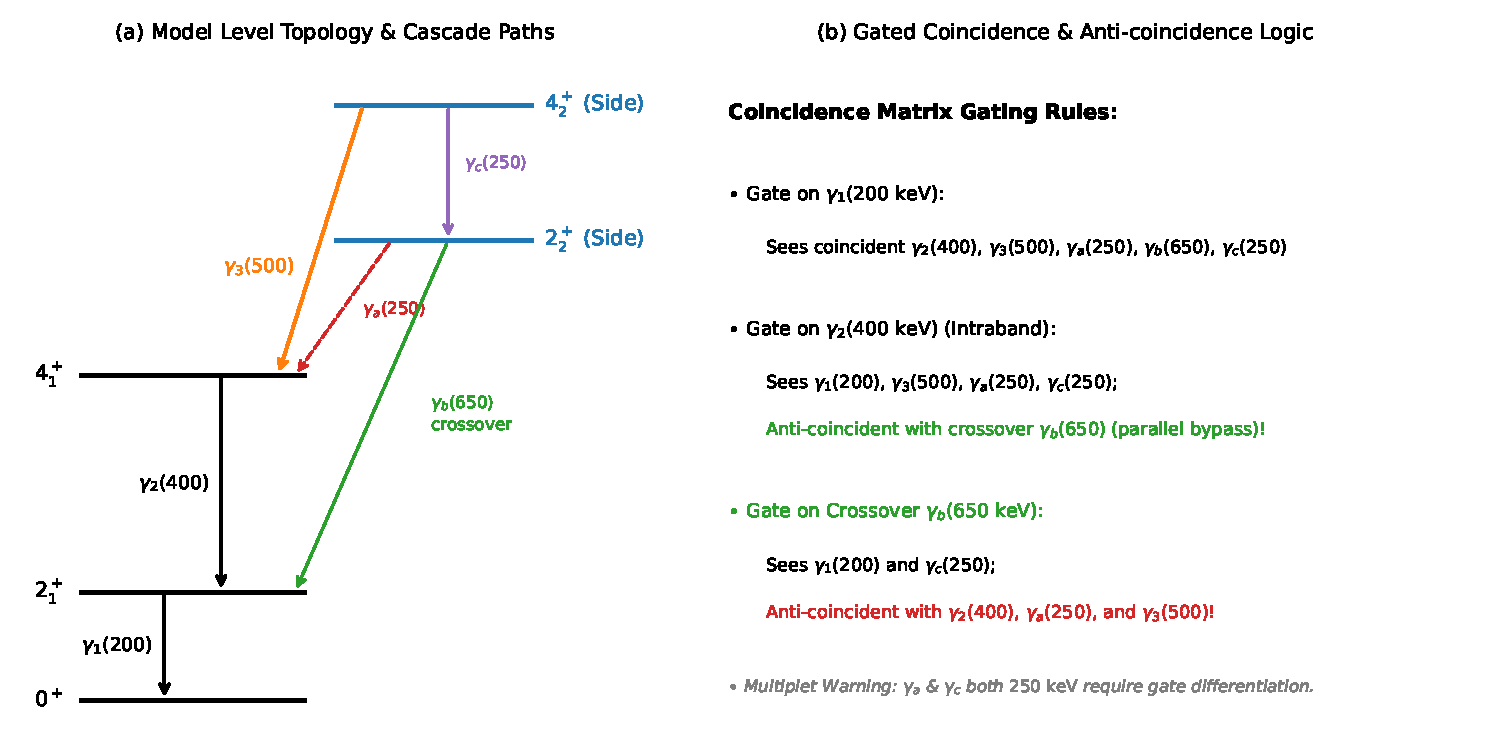
\includegraphics[width=0.92\textwidth]{Img/coincidence-level-scheme-model.pdf}%
\caption[典型核能级符合拓扑与门选反符合判据模型]{典型核能级符合拓扑与门选反符合判据模型（教学模型，基于参数化合成逻辑生成，各跃迁能量差、自旋多极选择定则及级联路径均经程序自洽验证）。(a) 展示包含基态带（$0^+ \to 2_1^+ \to 4_1^+$）与准 $\gamma$ 侧带（$2_2^+, 4_2^+$）的能级拓扑结构，包含带内与带间跃迁 $\gamma_1(200, E2), \gamma_2(400, E2), \gamma_3(500, M1+E2)$、侧向跃迁 $\gamma_a(250, E2), \gamma_c(250, E2)$ 以及交叉跃迁 $\gamma_b(650, M1+E2)$；(b) 给出符合门选逻辑：对 $\gamma_1$ 设门可见全部相连级联；对 $\gamma_2$ 设门可见 $\gamma_1, \gamma_3, \gamma_a, \gamma_c$，在理想衰变网络模型中与交叉跃迁 $\gamma_b$ 呈现拓扑反符合（平行旁路，无公共级联路径）；对交叉跃迁 $\gamma_b$ 设门可见 $\gamma_1, \gamma_c$，在理想模型中与 $\gamma_2, \gamma_a, \gamma_3$ 呈现拓扑反符合（在实验谱分析中，未观测到谱峰受探测限与统计涨落约束，与理想图模型的拓扑反符合性质有明确区分）；同时标示了 $\gamma_a$ 与 $\gamma_c$ 同为 $250\text{ keV}$ 时的双重峰（Doublet）门选消歧判据。注意此处为规范教学模型，非特定未知实验测量拟合）。}
\label{fig:5-6-coincidence-topology}
\end{figure}

\subsection{符合拓扑、级联排序与能级纲图建立原则}\label{subsec:5-6-5}

在谱学反演中必须牢记核心逻辑边界：\emph{两个特征 $\gamma$ 射线在谱图中存在符合关联，仅能证明二者同处于一个级联退激网络之中，并不自动确定二者的相对次序，更不代表二者是直接相连的相邻跃迁}。在排除反应伴生碎片、偶然相加与探测器散射串扰等假符合污染后，符合关系确认的是退激网络的拓扑连通性。从符合计数上升为可信能级纲图，必须同时满足以下拓扑闭合准则：
\begin{enumerate}
\item 能量守恒与 Ritz 组合原理（Ritz Combination Principle）：
在同一核素衰变网络中，两能级之间的能量差在计入微小的核反冲修正与实验刻度误差后，经由多步级联退激的跃迁能量代数和必须与交叉单跃迁（Crossover Transition）在测量不确定度内精确吻合。设各级联步跃迁能量为 $E_k$，反冲修正后的能级能量差为 $\Delta E_k = E_k + \frac{E_k^2}{2 M c^2}$，交叉跃迁对应能级差 $\Delta E_{\mathrm{crossover}} = E_{\mathrm{crossover}} + \frac{E_{\mathrm{crossover}}^2}{2 M c^2}$，则能量守恒要求 $\Delta E_{\mathrm{crossover}} = \sum_{k=1}^m \Delta E_k$。在观测光子能量尺度上，这表达为：
\begin{equation}\label{eq:5-6-ritz-combination}
E_{\mathrm{crossover}} = \sum_{k=1}^m E_k - \Delta E_{\mathrm{recoil}},
\end{equation}
其中 $\Delta E_{\mathrm{recoil}} \equiv \frac{E_{\mathrm{crossover}}^2}{2 M c^2} - \sum_{k=1}^m \frac{E_k^2}{2 M c^2} > 0$ 为交叉跃迁与多步级联反冲动能损失总和的差值（对于质量数 $A \approx 130$ 的核素，$1\,\text{MeV}$ 跃迁的反冲能量约为 $4\,\text{eV}$，在常规高分辨率高纯锗能谱中通常小于测量误差，但多步高能级联累积时仍应注意其物理定义）。
\item 强度平衡与开闭流分析：
在稳态衰变平衡与连续束流照射下，对中间能级 $|i\rangle$，其净布居速率由直接反应布居、侧向未观测馈入、离散级联注入与全部退激分支共同维持平衡：
\begin{equation}\label{eq:5-6-intensity-balance}
I_{\mathrm{direct}}(i) + I_{\mathrm{side}}(i) + \sum_{k} I_{\mathrm{tot}, k}^{\mathrm{in}} = \sum_{j} I_{\mathrm{tot}, j}^{\mathrm{out}} + I_{\mathrm{loss}}(i).
\end{equation}
仅在无直接输入且无未观测漏支的理想闭合子体系中，才近似有 $\sum I_{\mathrm{in}} \approx \sum I_{\mathrm{out}}$。总跃迁强度 $I_{\mathrm{tot}}$ 必须计入内转换系数 $\alpha_{\mathrm{IC}}$：
\begin{equation}\label{eq:5-6-itot-expansion}
I_{\mathrm{tot}, k} = I_{\gamma, k} (1 + \alpha_{\mathrm{IC}, k}).
\end{equation}
若某能级观测到的光子流入明显小于流出，常暗示存在来自高能连续区或侧带的未分辨馈入；若流入显著大于流出，则指示存在强内转换的未观测低能跃迁（$\alpha_{\mathrm{IC}} \gg 1$）。需要特别说明：在真正达到稳态且完全时间积分的闭合衰变网络中，总强度是严格守恒的，寿命本身并不会在稳态下消灭流量；若核态存在长寿命异能态延迟（$\tau_{\mathrm{isomer}} > \Delta T_{\mathrm{coin}}$）或处于脉冲束流的非稳态建立期，下游跃迁强度在有限时间门宽内将呈现表观的流入/流出不平衡，数据分析时须明确时间积分窗口与稳态建立的边界条件（肖骁 2019 硕士学位论文，PDF 第~24--26~页，印刷第~16--18~页~\cite{xiao-xiao-2019-high-spin-74as-thesis}）。
\item 级联次序的时间与强度反演：
单靠两个相互符合的光子能量无法确定相对上下次序。确定级联跃迁的上下次序依赖于强度单调递减规律（在无严重侧向注入的前提下，沿转动带自上而下退激时跃迁总强度单调累增）、从不同侧带分支汇入点的几何连接特征，以及第~5.4~节讨论的纳秒/皮秒时间差符合测量（若两态寿命差异足以在符合时间谱上分辨因果先后）。
\item 自旋宇称指定的独立证据输入：
能级纲图中每个激发态的自旋与宇称 $I^\pi$ 不能仅凭符合谱能量直接指认。能量符合建立的是能级拓扑连通图；能级自旋宇称的最终锁定，通常综合输入第~5.7~节的在束角分布 $W(\theta)$ / DCO（确定多极阶数 $L$ 与混合比 $\delta$）、Compton 偏振不对称度 / 内转换系数（确定电磁宇称性质 $\pi$），并结合已知的基态或基准能级锚定与选择定则。必须指出：自旋宇称指定的判定并不普遍要求测得能级绝对寿命 $\tau$。能级寿命 $\tau$ 与绝对折合跃迁几率 $B(XL)$ 是测定核结构波函数微观跃迁强度的关键物理量（见第~5.8~节），但由角分布与偏振给出的多极性与自旋指认属于辐射角动量与空间对称性约束，二者在实验证据链中具有明确的层次分工。
\end{enumerate}
通过符合拓扑、能量封闭、强度守恒与角分布偏振的多维交叉印证，才能将实验离线数据最终固化为经得起检验的确定核结构能级纲图。
%
}{%
    \section{符合矩阵与能级建立 [未完成]}\label{sec:5-6}%
    \textit{本节尚未完成。}%
}

%-- Section 5.7: 角关联、偏振和$\delta$反演
\setcounter{section}{6}%
\IfFileExists{Tex/Sections/sec-5-7.tex}{%
    \section{角关联、偏振和$\delta$反演}\label{sec:5-7}

在建立原子核能级纲图（第~5.6~节）之后，确定各能级的自旋宇称 $I^\pi$、鉴别电磁辐射的多极阶数（偶极 $L=1$ 或四极 $L=2$）以及提取电四极/磁偶极振幅混合比 $\delta(E2/M1)$，构成了在束 $\gamma$ 谱学向微观核结构模型（如转子模型、粒子-转子耦合与手征/摆动动力学）过渡的核心纽带。单纯的 $\gamma$ 跃迁能量与符合连接仅能提供能级拓扑连通性，无法独立锁定量子态的角动量与宇称。

在束重离子反应在自旋排列方向上具有天然的各向异性（见第~5.1~节）。出射 $\gamma$ 射线的空间角分布、双探测器方向角关联（DCO）以及康普顿线偏振度，携带着辐射场多极性与跃迁几率振幅干涉相位的直接信息。然而，由宏观角分布与偏振反演微观多极混合比 $\delta$ 是一类典型的非线性反问题。若对相位约定、退取向衰减、门选条件以及二次有理方程的多解特性缺乏严格界定，极易在谱学推断中产生两类典型偏差：其一，将特定几何下的 DCO 比值经验数值（如 1.0 或 0.5）当成普遍适用的多极性分界线，忽略门跃迁多极性与自旋序列的调制；其二，在角分布方程存在两个相容数学根时，依据理论模型的偏好人为舍弃其中一个物理自洽解分支，将理论假设冒充为独立实验判决。本节从统计取向张量与角分布几何展开出发，严格定义实多极混合比 $\delta$ 的相位约定，推导条件 DCO 强度比与康普顿散射偏振度方程，建立似然剖面下的双根反演与多解仲裁准则。

\subsection{角动量取向、辐射场几何与角分布理论}\label{subsec:5-7-1}

在束重离子完全熔合蒸发反应中，由于入射相对运动轨道角动量强烈偏向于垂直于束流轴的平面，初始复合核的磁子能级呈现高度取向的不均匀分布。在经历了相继的轻核子蒸发与统计非共振 $\gamma$ 级联后，待测母能级 $|i\rangle$（自旋为 $I_i$）可以保留一定程度的、沿束流轴（定为量子化 $z$ 轴）的轴对称取向。

母态的自旋取向状态由统计取向张量（Orientation Tensor）$B_k(I_i)$ 描述（Hamilton 1975 经典专著规范~\cite{book-hamilton-electromagnetic-interaction}）：
\begin{equation}\label{eq:5-7-bk-def}
B_k(I_i) \equiv \sqrt{2I_i + 1} \sum_{M_i} (-1)^{I_i - M_i} \langle I_i M_i I_i (-M_i) \mid k 0 \rangle P(M_i),
\end{equation}
其中 $P(M_i)$ 为磁子能级 $M_i$ 的统计布居几率，且满足归一条件 $\sum_{M_i} P(M_i) = 1$。由 Clebsch-Gordan 系数正交归一性，张量零阶项 $B_0(I_i) \equiv 1$ 对任意归一布居分布 $P(M_i)$ 恒成立（并不限于各向同性分布）。式中 Clebsch-Gordan 系数的次序规定了统计张量的相位约定；与 Hamilton 式~(12.73) 的张量记号相比，按式~\eqref{eq:5-7-bk-def} 定义的奇阶分量满足 $B_k = (-1)^k B_k^{\mathrm{Hamilton}}$，偶阶分量严格相同。

沿束流轴的轴对称性保证方位角量子数 $q = 0$（无非对角取向张量）。在所选量子化基中，若磁子能级布居满足非定向排列（Alignment）对称性 $P(M_i) = P(-M_i)$，则奇阶取向张量严格为零（$B_{\mathrm{odd}} = 0$）；若存在非对称极化（Polarization, $P(M_i) \ne P(-M_i)$），奇阶张量（如 $B_1$）可以非零。必须强调，对具有确定宇称的核态之间的通常电磁单光子跃迁，未分析光子偏振时需对两个出射螺旋度（$\lambda = \pm 1$）求和，强度分布中的奇阶辐射参数因螺旋度求和而严格抵消，因此强度级数中的奇阶贡献恒为零，即使母态本身具有非零奇阶取向张量也是如此（Hamilton 式~(12.180)--(12.189)）。受出射辐射场多极阶数（$L, L' \le L_{\max}$）与态自旋的三角选择定则双重限制，张量阶数截断于 $k \le \min(2I_i, 2L_{\max})$；对于最高多极阶数为四极（$L_{\max}=2$）的情形，强度展开式最多仅包含偶阶项 $k = 0, 2, 4$。

若母态是由一条指定的、未被探测的前级级联退激至 $I_i$，前级未观测级联退取向在单一路径下由去取向因子 $U_k = \prod_m U_k(m)$ 描述：
\begin{equation}\label{eq:5-7-deorientation}
B_k(I_i) = B_k(J_{\mathrm{CN}}) \prod_m U_k(m),
\end{equation}
若存在多条可能馈入路径，则应依据各分支布居份额加权求和。特别注意：若后文已直接使用目标母态的统计取向张量 $B_k(I_i)$，则其已内含了所有上游未观测级联的退取向效应，绝不可在后续角分布或表观展开系数中再次重复乘以相同的 $U_k$。

从取向母态 $|i\rangle$ 退激至末态 $|f\rangle$（自旋 $I_f$）发射的单色 $\gamma$ 射线，其相对于束流轴夹角 $\theta$ 的相对角分布函数 $W(\theta)$ 展开为偶阶 Legendre 多项式序列：
\begin{equation}\label{eq:5-7-w-theta-general}
W(\theta) = \sum_{k=0, 2, 4} B_k(I_i) A_k(\delta) Q_k P_k(\cos\theta),
\end{equation}
其中：
\begin{itemize}
\item $P_k(\cos\theta)$ 为标准第 $k$ 阶 Legendre 多项式（$P_0 = 1$，$P_2 = \frac{1}{2}(3\cos^2\theta - 1)$，$P_4 = \frac{1}{8}(35\cos^4\theta - 30\cos^2\theta + 3)$）；
\item $Q_k$ 为探测器对源张开有限立体角引起的几何衰减因子（Finite Solid-Angle Correction Factor），定义为 $Q_k = \int w(\Omega) P_k(\cos\alpha) d\Omega / \int w(\Omega) d\Omega$。作为标量因子的简化表示仅在探测效率分布 $w(\Omega) \ge 0$ 绕探测器中心晶体对称轴轴对称时严格成立（一般非轴对称几何须进行全立体角多极响应积分），满足 $Q_0 = 1$ 与 $|Q_k| \le 1$；
\item $A_k(\delta)$ 为由跃迁多极类型与多极混合比决定的辐射角分布系数；
\item 截断阶数 $k \le 4$ 建立在出射辐射场多极性不超过四极（$L, L' \le 2$）的基础之上（由选择定则 $k \le \min(2I_i, 2L_{\max})$ 严格限定）。
\end{itemize}
在实验数据分析中，角分布通常拟合为常规 Legendre 展开形式：
\begin{equation}\label{eq:5-7-w-theta-fit}
W(\theta) = 1 + a_2 P_2(\cos\theta) + a_4 P_4(\cos\theta),
\end{equation}
其中表观展开系数满足
\begin{equation}\label{eq:5-7-ak-apparent}
a_k = \frac{B_k(I_i) Q_k A_k(\delta)}{B_0(I_i) Q_0 A_0} = B_k(I_i) Q_k A_k(\delta),\qquad k=2,4,
\end{equation}
第二个等号采用了 $B_0(I_i) = Q_0 = A_0 = 1$ 的标准归一约定。此处 $B_k(I_i)$ 已直接表征待测态的实际取向度，式中绝无重复的 $U_k$ 因子。

\subsection{多极混合比$\delta$的相位约定与二次有理展开}\label{subsec:5-7-2}

当跃迁在角动量三角定则与宇称守恒下允许低阶辐射多极 $L$ 与高阶辐射多极 $L' = L + 1$ 同时存在时（最常见的是磁偶极 $M1$ 与电四极 $E2$ 竞争跃迁），出射场呈现多极相干叠加。

必须对实多极混合比 $\delta$ 给出严格的无量纲辐射几率振幅比定义。本节与第~5.9~节（式~\eqref{eq:5-9-delta-def}）及附录~A（式~\eqref{eq:appA-delta-def}）统一采用 Krane--Steffen（KS）多极混合比规范体系~\cite{lange-kumar-hamilton-1982-multipole-admixtures, book-hamilton-electromagnetic-interaction}：
\begin{equation}\label{eq:5-7-delta-def}
\delta(E2/M1) \equiv \frac{\gamma(E2)}{\gamma(M1)} = \frac{\sqrt{3}}{10} \frac{E_\gamma}{\hbar c} \frac{\langle I_f \| \mathcal{M}(E2) \| I_i \rangle}{\langle I_f \| \mathcal{M}_S(M1) \| I_i \rangle} = \frac{\sqrt{3}}{10} \frac{E_\gamma}{\hbar} \frac{\langle I_f \| \mathcal{M}(E2) \| I_i \rangle}{\langle I_f \| \mathcal{M}_\mu(M1) \| I_i \rangle}.
\end{equation}
在此定义下：
\begin{itemize}
\item $\delta$ 是出射光子场的电四极振幅与磁偶极振幅之比，是严格的无量纲纯数；
\item 它不是裸约化矩阵元的简单相比，而是内含了跃迁动量因子 $k_\gamma = E_\gamma / (\hbar c)$ 与相应的常数因子。当分母采用 SI 电荷型算符 $\mathcal{M}_S(M1) \equiv \mathcal{M}_\mu(M1) / c$ 时，其量纲为 $e\cdot\mathrm{fm}$，分子 $\mathcal{M}(E2)$ 量纲为 $e\cdot\mathrm{fm}^2$，动量因子 $E_\gamma/(\hbar c)$ 量纲为 $\mathrm{fm}^{-1}$，实现量纲严格对消；当分母采用磁矩型算符 $\mathcal{M}_\mu(M1)$（量纲 $\mu_N$）时，频率因子相应为 $E_\gamma/\hbar$，与第~5.9~节及附录~A 保持统一量纲与符号，避免无谓的单位重复折算；
\item 初末态波函数的全同规范位相在比值中精确对消，$\delta$ 的符号由跃迁算符定义与物理矩阵元内禀结构共同锁定。
\end{itemize}

在文献转换中，必须注意不同历史相位约定的映射关系：
除 Krane--Steffen（KS）约定外，核物理谱学还存在 Rose--Brink（RB）约定与 Biedenharn--Rose（BR）约定。在 Lange 等人~\cite{lange-kumar-hamilton-1982-multipole-admixtures} 给出的发射退激约定下，Krane--Steffen 约定与 Rose--Brink 约定的实数混合比相差一个负号：$\delta_{\mathrm{KS}} = -\delta_{\mathrm{RB}}$。\emph{若将文献中的 $\delta$ 符号转换至另一体系，必须同时将角分布干涉项系数的定义进行同步转换；绝不能在保留原公式几何系数形式的同时单独强行翻转 $\delta$ 的正负号}。

对于纯 $L$ 辐射与 $L'=L+1$ 辐射的混合，辐射角分布系数 $A_k(\delta)$ 可严格表征为混合比 $\delta$ 的二次有理函数~\cite{lange-kumar-hamilton-1982-multipole-admixtures}：
\begin{equation}\label{eq:5-7-ak-rational}
A_k(\delta) = \frac{F_k(L L I_f I_i) + 2\delta F_k(L L' I_f I_i) + \delta^2 F_k(L' L' I_f I_i)}{1 + \delta^2},
\end{equation}
其中 $F_k(L L' I_f I_i)$ 为纯几何性质的 Ferentz-Rosenzweig 系数（由 Racah 代数与 Wigner $6j$ 符号精确确定，其定义见Hamilton印539/PDF550式(12.168)）。对于最核心的 $M1+E2$ 跃迁（$L=1, L'=2$），式~\eqref{eq:5-7-ak-rational} 表达为：
\begin{equation}\label{eq:5-7-ak-m1e2}
A_k(\delta) = \frac{F_k(1 1 I_f I_i) + 2\delta F_k(1 2 I_f I_i) + \delta^2 F_k(2 2 I_f I_i)}{1 + \delta^2}.
\end{equation}
分子中的交叉项 $+2\delta F_k(1 2)$ 直观展示了电四极与磁偶极发射振幅之间的量子力学相干干涉。在 Hamilton 专著与 Lange 等人的公式体系中，该正干涉交叉项严格对应于 Krane--Steffen 约定，绝不可将其直接标为 Rose--Brink 公式。

\subsection{定向态方向角关联（DCO）与门谱几何修正}\label{subsec:5-7-3}

虽然一维角分布 $W(\theta)$ 理论优美，但在重离子在束实验中，直接测量单谱角分布往往受到靶核连续本底与杂质峰的严重干扰。在多探测器阵列中，更常用的实验方法是在二维符合矩阵（第~5.6~节）上建立\emph{定向态方向角关联}（Directional Correlation from Oriented States, DCO）。

考虑由级联跃迁 $\gamma_1$ 与 $\gamma_2$ 构成的符合事件。实验将探测器分别放置在特定的两个极角 $\theta_1$ 与 $\theta_2$（相对于束流轴，通常选取 $90^\circ$ 与前向/后向角度如 $30^\circ$ 或 $135^\circ$）。由非对称符合矩阵（见第~5.6~节的非对称矩阵定义）导出的实验 DCO 比值严格定义为条件门选强度之比：
\begin{equation}\label{eq:5-7-dco-def}
R_{\mathrm{DCO}} \equiv \frac{N_{\gamma 1, \gamma 2}(\theta_1, \theta_2)}{N_{\gamma 1, \gamma 2}(\theta_2, \theta_1)} \times \frac{\varepsilon_{\mathrm{p}}(\theta_2, E_{\gamma 1}) \varepsilon_{\mathrm{p}}(\theta_1, E_{\gamma 2})}{\varepsilon_{\mathrm{p}}(\theta_1, E_{\gamma 1}) \varepsilon_{\mathrm{p}}(\theta_2, E_{\gamma 2})},
\end{equation}
其中 $\varepsilon_{\mathrm{p}}(\theta, E)$ 为该角度通道的绝对全能峰探测效率。式~\eqref{eq:5-7-dco-def} 使用同一套计数、门宽、束流曝光和本底扣除约定，并假定角组的双探测效率可由所列单探测效率乘积表示；若角组由多对探测器构成或存在通道间响应关联，需以各探测器对的实际响应加权计算。

必须澄清针对 DCO 比值的方法学常见误区：
\begin{enumerate}
\item DCO 比值绝非单谱角分布比值 $W(\theta_1)/W(\theta_2)$：
门跃迁 $\gamma_2$ 可以位于待测跃迁 $\gamma_1$ 之前（前级馈入门），亦可位于其后（后续退激出射门）；双光子定向角关联理论函数必须依据级联跃迁的实际时间发射次序由 Racah 统计重耦合理论严格构造（Hamilton 专著第~12~章式~(12.199)~\cite{book-hamilton-electromagnetic-interaction}），不可将所有门选笼统等同于对中间态的静态重排。
\item 不存在通用的“DCO 等于 1.0 即为四极、等于 0.5 即为偶极”的绝对分界：
理论 $R_{\mathrm{DCO}}$ 的数值强烈依赖于门跃迁 $\gamma_2$ 的多极性质与自旋变化：
\begin{itemize}
\item 若门跃迁 $\gamma_2$ 为拉伸四极跃迁（$\Delta I = 2$ 纯 $E2$），在典型几何（如 $\theta_1 = 30^\circ, \theta_2 = 90^\circ$）下，待测跃迁若是拉伸四极（$\Delta I = 2$ 纯 $E2$），$R_{\mathrm{DCO}} \approx 1.0$；若待测跃迁为纯偶极（$\Delta I = 1$），$R_{\mathrm{DCO}} \approx 0.6$ 左右；
\item 若门跃迁 $\gamma_2$ 本身改为纯偶极跃迁（$\Delta I = 1$），基准参考值发生倒置——此时纯四极待测跃迁的 $R_{\mathrm{DCO}} \approx 1.7$ 左右，而纯偶极待测跃迁的 $R_{\mathrm{DCO}} \approx 1.0$。
\end{itemize}
\item 剩余自旋取向宽度的影响：
实际重离子实验中母态取向受高斯分布宽度参数 $\sigma/I$ 调制。未知的级联退取向与侧向馈入会压低偏离各向同性的幅度，在反演分析中取向宽度可通过已知纯 $E2$ 跃迁标定、理论反应道约束、联合拟合或系统误差包络进行稳健评估。
\end{enumerate}

\subsection{康普顿散射偏振度与电磁宇称仲裁}\label{subsec:5-7-4}

角分布与 DCO 比值主要敏感于多极阶数 $L$ 与自旋变化 $\Delta I$，但在鉴别出射光子的电磁宇称性质（例如区分属于宇称翻转的电偶极 $E1$（宇称选择定则 $\pi_i \pi_f = (-1)^L = -1$）还是宇称不变的磁偶极 $M1$（$\pi_i \pi_f = (-1)^{L+1} = +1$））时通常不具备区分能力。线偏振度（Linear Polarization）可以提供额外约束；内转换系数或独立宇称锚点也可发挥作用，并非所有指定都必须依赖偏振测量。

利用 Clover 探测器中 4 块相互正交晶体构成的微型康普顿偏振计（第~5.2~节式~\eqref{eq:5-2-klein-nishina-pol}），光子发生康普顿散射的截面强烈偏向于垂直于电矢量 $\mathbf{E}$ 的方位平面。实验测得的散射不对称度为：
\begin{equation}\label{eq:5-7-asym-exp}
A_{\mathrm{exp}} = \frac{N_\perp - a(E_\gamma) N_\parallel}{N_\perp + a(E_\gamma) N_\parallel},
\end{equation}
其中 $N_\parallel$ 与 $N_\perp$ 分别为光子在平行于核反应平面（由束流轴与光子发射方向确定）与垂直于核反应平面内散射进入相邻晶体的计数，$a(E_\gamma) = N_\perp^{\mathrm{unpol}} / N_\parallel^{\mathrm{unpol}}$ 为利用无偏振放射源实验标定的仪器几何与探测效率固有不对称校正系数。

线偏振度 $P$ 表达为实验不对称度与偏振灵敏度因数（Analyzing Power）$Q(E_\gamma)$ 之比：
\begin{equation}\label{eq:5-7-pol-degree}
P = \frac{A_{\mathrm{exp}}}{Q(E_\gamma)},\qquad Q(E_\gamma)\ne0,
\end{equation}
其中 Clover 探测器的偏振分析能力 $Q(E_\gamma)$ 依赖于光子能量与晶体间距以及实际散射接受条件，需用已知偏振度的校准跃迁或经核验的响应计算确定。偏振分析本领 $Q(E_\gamma)$ 与角分布立体角因子 $Q_k$ 均为无量纲量，但前者联系散射不对称与入射偏振，后者描述角接受对各阶展开的平均衰减，使用时应分别标定和定义。

在取向核跃迁理论中，相对于核反应平面的线偏振度 $P(\theta)$ 严格定义为平行与垂直电矢量偏振分量的强度相对不对称：
\begin{equation}\label{eq:5-7-pol-def}
P(\theta) \equiv \frac{W_\parallel(\theta) - W_\perp(\theta)}{W_\parallel(\theta) + W_\perp(\theta)}.
\end{equation}
依据经典辐射场偏振理论展开（Hamilton 1975 专著第~12~章式~(12.198) 与第~15~章式~(15.9)--(15.15) 规范~\cite{book-hamilton-electromagnetic-interaction}），$P(\theta)$ 表达为关联 Legendre 展开形式：
\begin{equation}\label{eq:5-7-pol-theor}
P(\theta) = \frac{\sum_{k \ge 2, \,\mathrm{even}} B_k(I_i) A_k^{\mathrm{pol}}(\delta) Q_k^{\mathrm{pol}} P_k^2(\cos\theta)}{\sum_{k \,\mathrm{even}} B_k(I_i) A_k(\delta) Q_k P_k(\cos\theta)},
\end{equation}
其中分母即为未分析偏振的单色总辐射角分布 $W(\theta) = W_\parallel(\theta) + W_\perp(\theta)$，分子中的 $P_k^2(\cos\theta)$ 为标准第 $k$ 阶缔合 Legendre 多项式（$P_2^2(\cos\theta) = 3\sin^2\theta$，$P_4^2(\cos\theta) = \frac{15}{2}\sin^2\theta(7\cos^2\theta - 1)$）。若采用 Hamilton 所定义的偏振系数 $A_{k2}$，展开系数中须包含归一化因子 $2\sqrt{\frac{(k-2)!}{(k+2)!}}$（对 $k=2$ 该因子为 $2/\sqrt{24} = 1/\sqrt{6}$；对 $k=4$ 为 $2/\sqrt{360} = 1/\sqrt{90}$）。本节将该系数吸收入 $A_k^{\mathrm{pol}}=2\sqrt{(k-2)!/(k+2)!}\,A_{k2}$。$Q_k^{\mathrm{pol}}$ 表示与偏振张量相容的有限立体角接受衰减因子。

在相同自旋序列下，纯电性多极辐射与纯磁性多极辐射的线偏振度呈现符号反转（例如 $\Delta I = 1$ 的纯电偶极 $E1$ 偏振度通常为正，而同序列纯磁偶极 $M1$ 偏振度为负）。但对于 $M1+E2$ 混合跃迁，偏振度由两多极分量的干涉二次式确定，\emph{偏振度 $P$ 为正绝不等于直接证明跃迁必为纯 $E2$ 辐射}。混合态的偏振符号与幅度强烈依赖于具体角度 $\theta$、自旋变化 $\Delta I$ 以及混合比 $\delta$ 的实际取值。

\subsection{似然剖面、多解双根与物理分支仲裁}\label{subsec:5-7-5}

由于辐射角分布系数 $A_k(\delta)$（式~\eqref{eq:5-7-ak-m1e2}）与实验 DCO 比值 $R_{\mathrm{DCO}}(\delta)$ 关于多极混合比 $\delta$ 均为二次有理函数：
\begin{equation}\label{eq:5-7-dco-rational}
R_{\mathrm{DCO}}(\delta) = \frac{N(\delta)}{D(\delta)} = \frac{n_0 + n_1 \delta + n_2 \delta^2}{d_0 + d_1 \delta + d_2 \delta^2},
\end{equation}
其中展开系数由探测角几何、初末态自旋序列及门跃迁多极性由双光子角关联理论确定。将实测 $R_{\mathrm{DCO}}$ 代入并交叉相乘后，得到关于 $\delta$ 的代数方程：
\begin{equation}\label{eq:5-7-quadratic-roots}
c_2 \delta^2 + c_1 \delta + c_0 = 0,
\end{equation}
其中二次有理反演系数为 $c_2 = n_2 - R_{\mathrm{DCO}} d_2$，$c_1 = n_1 - R_{\mathrm{DCO}} d_1$，$c_0 = n_0 - R_{\mathrm{DCO}} d_0$。

式~\eqref{eq:5-7-quadratic-roots} 的求解必须遵守严格的代数与物理边界：
\begin{itemize}
\item \textbf{排除分母为零的伪根}：式~\eqref{eq:5-7-quadratic-roots} 是在两端同乘以分母 $D(\delta)$ 得到的必要条件。求得的任何有限实根 $\delta^*$，必须代回原始分母验证 $D(\delta^*) \ne 0$。若代数方程的某个根使得原始分母为零（$D(\delta^*) = 0$），该点属于去分母引入的无意义伪根，必须严格予以剔除。
\item \textbf{齐次投影坐标与纯多极端点}：引入齐次坐标 $\delta = u/v$（$v \ne 0$ 时 $\delta = u/v$，并对应有界相角 $\theta_\delta \equiv \arctan(u/v) \in [-\pi/2, \pi/2]$），代数方程改写为齐次二次型：
\begin{equation}\label{eq:5-7-projective-form}
(n_2 - R_{\mathrm{DCO}} d_2) u^2 + (n_1 - R_{\mathrm{DCO}} d_1) uv + (n_0 - R_{\mathrm{DCO}} d_0) v^2 = 0.
\end{equation}
纯高阶多极极限（如纯 $E2$，$L'=2$）对应于 $v=0$（即 $|\delta| \to \infty$ 或 $\theta_\delta = \pm 90^\circ$）。当 $d_2 \ne 0$ 且实测值 $R_{\mathrm{DCO}} = n_2 / d_2$ 时，代数方程在 $v=0$ 处精确满足！在这里 $d_2\ne0$ 的适用条件下，极限端点 $\delta \to \pm\infty$ 不是物理响应比值的奇异极点（Poles），因为物理强度比值在无穷远具有良好有限极限 $\lim_{|\delta| \to \infty} R_{\mathrm{DCO}}(\delta) = n_2 / d_2$；且两个端点 $\theta_\delta = +90^\circ$ 与 $-90^\circ$ 在物理上代表同一个纯高阶辐射振幅态（由于多极几率由平方项决定，二者物理不可分辨并折叠为同一状态）。
\item \textbf{退化与一次方程分析}：当 $c_2 = 0$ 但 $c_1 \ne 0$ 时，方程退化为一次代数方程，仅存在单一有限解 $\delta = -c_0/c_1$（需满足 $D(\delta) \ne 0$），此时需结合齐次形式另行检验 $v=0$ 纯多极端点是否构成本质解；若 $c_2 = c_1 = 0$ 且 $c_0 \ne 0$，在有限实数域无解，但仍需检查齐次端点及其原始响应是否定义；若 $c_2 = c_1 = c_0 = 0$，则分子分母成常数倍数（$N(\delta) \equiv R_{\mathrm{DCO}} D(\delta)$），在定义域内任意有限 $\delta$ 均完全简并。
\item \textbf{相容实根分支保留准则}：在非退化二次情形下，当判别式 $\Delta = c_1^2 - 4 c_2 c_0 \ge 0$ 时，方程在实数域给出 1 个或 2 个有限实数根。当存在两个实根时，两根并不必然表现为一小一大，其拟合优度亦未必相同；偏振测量或内转换系数能够提供独立的鉴别条件，但在缺乏附加实验数据时，不可无故断言某一根已被排除。
\end{itemize}

为向读者直观展示这一二次反演多解特征及偏振的裁决机制，图~\ref{fig:5-7-angular-branch} 给出了规范教学模型的解析曲线与双根相交示意图。

\begin{figure}[!htbp]
\centering
%
  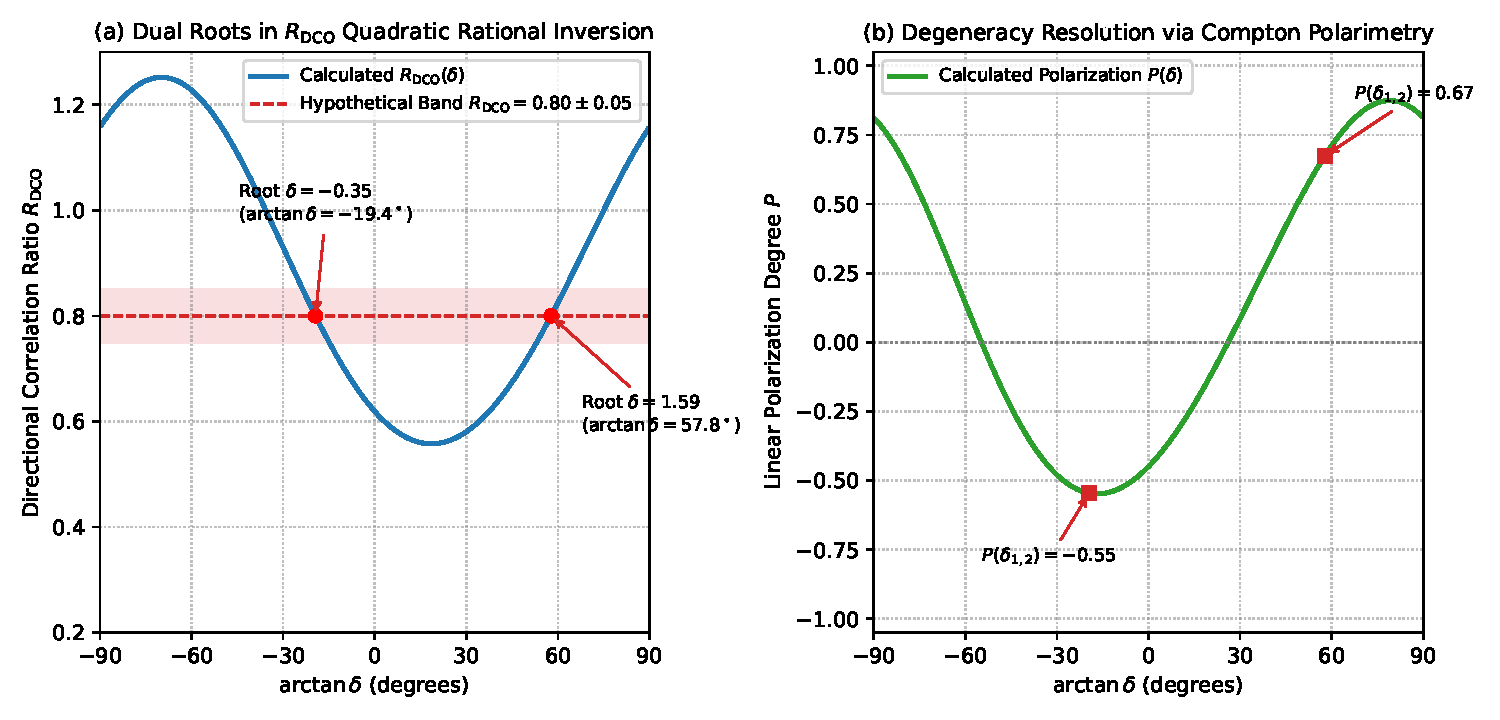
\includegraphics[width=0.92\textwidth]{Img/angular-branch-delta-likelihood.pdf}%
\caption[多极混合比 $\delta$ 的二次有理反演与偏振简并解除机制]{多极混合比 $\delta$ 的二次有理反演与偏振简并解除机制（规范教学模型）。(a) 展示由严格正定响应比值构造的 $R_{\mathrm{DCO}}(\delta)$ 关于 $\arctan\delta$ 的二次有理示意曲线（系数选取保证分子与分母在全实数域恒为正），水平阴影带代表假设观测带 $R_{\mathrm{DCO}} = 0.80 \pm 0.05$。假设带与曲线相交给出两个完全相容的数学根分支 $\delta_1 = -0.35$（$\arctan\delta_1 = -19.4^\circ$）与 $\delta_2 = +1.59$（$\arctan\delta_2 = +57.8^\circ$）；(b) 给出满足正交偏振强度非负条件（$W \pm H > 0$，即 $|P| < 1$ 恒成立）的示意线偏振度 $P(\delta)$ 理论曲线。在两个根位置偏振度呈现显著差异（在这组自选系数下，$P(\delta_1)\approx-0.55$、$P(\delta_2)\approx+0.67$；实际电磁归属仍须结合自旋序列和响应模型），直观说明仅靠 DCO 比值无法独立定解，在测量不确定度与探测灵敏度具备足够区分力时，可借助康普顿散射偏振计或内转换电子谱区分两支解；这些不同响应约束在统计上是否独立，仍须核对共同事件与校准。注意此处曲线为代数构造的自洽规范教学模型，用于阐释方法学原理，非特定核态或探测硬件的实测拟合。}
\label{fig:5-7-angular-branch}
\end{figure}

图~\ref{fig:5-7-angular-branch} 确立了低能核结构谱学分析的一条关键证据边界：
\begin{enumerate}
\item 独立实验数据的分支保留原则：
在仅有角分布或 DCO 比值测量、缺乏具有足够区分精度的偏振度或内转换系数数据时，\emph{应报告所有仍与数据相容的分离分支及各自误差}！
\item 理论模型偏好不得冒充独立实验判决：
在核结构理论比对中（例如轴对称刚性转子模型或三轴粒子-转子耦合模型），模型往往预言特定带间跃迁具有极小的 $\delta$ 或特定的四极主导性。研究人员绝不能为了迎合某种理论偏好，在实验报告中人为剔除另一个与数据相容的候选根。
\item 连续似然剖面（Likelihood Profile）构建：
在统计推断中，可通过构建轮廓似然比检验曲线 $-2\Delta\ln \max_{\boldsymbol{\eta}} \mathcal{L}(\delta, \boldsymbol{\eta}) + \text{const}$，其参考分布与置信度需按实际统计模型确定；满足渐近正则性时可采用相应的卡方标尺；若原始矩阵包含非泊松结构或系统协方差，而已发表观测矢量 $\mathbf{y}$、响应均值模型及协方差矩阵 $\mathbf{V}$ 足以支撑声明的误差近似，广义最小二乘仍可作为推断框架；它不自动保证非高斯、小样本或奇异协方差下的区间覆盖，需按实际模型处理约束并校准。由于 $\delta$ 在实数轴上可延伸至 $\pm \infty$，通常在有界坐标 $\theta_\delta \equiv \arctan\delta \in [-\pi/2, \pi/2]$ 上绘制全局拟合剖面，展示可能呈现的双极小值结构及其非对称置信区间，并将其作为后续第~5.10~节全篇测量模型整合的客观输入。
\end{enumerate}

以奇 $A$ 核 $^{163}\mathrm{Lu}$ 中三轴超形变摆动带（TSD）的研究为例（A. Görgen 等人 2004 年经典工作~\cite{campaign-g07-gorgen-2004-163lu-quadrupole-moments}），在反演 TSD2 向 TSD1 带间跃迁的绝对 $B(E2)_{\mathrm{out}}$ 与 $B(M1)_{\mathrm{out}}$ 几率时，作者直接借用了先前独立薄靶角关联与偏振实验测得的平均值 $\delta = -3.10^{+0.36}_{-0.44}$，并假定其在整个高自旋带保持稳定。必须澄清：该文自身并未在此厚靶高自旋测量中重新独立测定高自旋各态的偏振度，而是基于共享的先前实验输入；这一实例表明微观多极强度反演往往依赖于先验假定与外部辅助测量。

% 额外观测提供不同响应约束；统计独立性仍须核对共同事件与校准。
%
}{%
    \section{角关联、偏振和$\delta$反演 [未完成]}\label{sec:5-7}%
    \textit{本节尚未完成。}%
}

%-- Section 5.8: DSAM与RDDS的时间信息
\setcounter{section}{7}%
\IfFileExists{Tex/Sections/sec-5-8.tex}{%
    \section{DSAM与RDDS的时间信息}\label{sec:5-8}

在从微观能级结构向电磁约化跃迁几率 $B(XL)$ 反演的因果链中（第~5.9~节），激发能级的平均寿命 $\tau$ 构成了最为关键的时间标尺。跃迁率与寿命之间满足基本的反比关系 $\lambda_{\mathrm{tot}} = 1/\tau$；若无法精确测定激发能级的微观寿命，仅凭相对分支比与角分布无法解耦出绝对的微观跃迁矩阵元模平方。

在在束 $\gamma$ 谱学实验中，皮秒（$\text{ps}$）至飞秒（$\text{fs}$）量级的超快核跃迁远远超出了常规电子学时间数字转换器（TDC）或恒比定时（CFD）通道的直接物理时间分辨率（通常约为几百皮秒至纳秒量级）。为了突破这一硬件时间测量极限，现代实验谱学普遍利用核反应产生的高速反冲核在真空飞行或固体介质慢化过程中产生的时间--空间多普勒频移特征，分别发展了反冲距离多普勒频移法（Recoil Distance Doppler-Shift, RDDS）以及多普勒频移衰减法（Doppler Shift Attenuation Method, DSAM）~\cite{dewald-2012-ddcm-recoil-distance, book-wu-nuclear-experiment-methods}。

若对多普勒几何变换、减速介质阻止本领（Stopping Power）模型、微分衰变曲线法（DDCM）以及侧向馈入时间卷积缺乏清晰界定，极易在寿命反演中引入显著的系统性偏置：例如混淆静止系发射角与实验室观测角导致多普勒频移计算失真，在直接符合门中错误将飞行发射假定为离靶瞬间布居，或者在减速截面存在理论不确定度时低估 DSAM 寿命误差。本节从相对论多普勒几何出发，推导 RDDS 的飞行时间映射与 DDCM 解析方程，系统剖析 DSAM 谱形展宽的连续慢化与停止截面机制，界定各测时技术的敏感窗口与适用边界，为第~5.9~节绝对跃迁强度的精确提取提供可追溯的时间信息基础。

\subsection{多普勒效应与相对论变换几何}\label{subsec:5-8-1}

考虑在核反应中获得反冲初速度 $\mathbf{v}$ 的激发态残核，其在实验室参考系中相对光速的比值为 $\boldsymbol{\beta} = \mathbf{v}/c$，对应的相对论 Lorentz 因子为 $\gamma = 1/\sqrt{1 - \beta^2}$。设该原子核在其静止参考系中退激发射一个固有能量为 $E_0$ 的单色 $\gamma$ 光子。

在实验室参考系中，探测器位于相对于反冲速度矢量夹角为 $\theta_{\mathrm{lab}}$ 的方向。由四维波矢量的标准 Lorentz 变换，实验室系测得的光子能量 $E_{\mathrm{obs}}$ 满足相对论多普勒频移公式~\cite{dewald-2012-ddcm-recoil-distance}：
\begin{equation}\label{eq:5-8-doppler-rel}
E_{\mathrm{obs}} = \frac{E_0}{\gamma (1 - \beta \cos\theta_{\mathrm{lab}})}.
\end{equation}
在此必须注意角动量变换几何：式~\eqref{eq:5-8-doppler-rel} 中的极角 $\theta_{\mathrm{lab}}$ 是实验室系中的实际观测角度，不可将其与原子核静止系中的发射角 $\theta_{\mathrm{rest}}$ 相混淆（二者满足相对论光行差关系 $\cos\theta_{\mathrm{rest}} = \frac{\cos\theta_{\mathrm{lab}} - \beta}{1 - \beta\cos\theta_{\mathrm{lab}}}$）。

在典型的低能核结构重离子熔合反应中，反冲核速度通常较小（典型范围为 $\beta \sim 1\%$–$3\%$）。在低速非相对论极限（$\beta \ll 1$）下，对式~\eqref{eq:5-8-doppler-rel} 按 $\beta$ 进行一阶展开：
\begin{equation}\label{eq:5-8-doppler-approx}
E_{\mathrm{obs}} \approx E_0 (1 + \beta \cos\theta_{\mathrm{lab}}).
\end{equation}
低速近似下，探测器在前进方向（$\theta_{\mathrm{lab}} = 0^\circ$）测得最大蓝移能量 $E_{\max} \approx E_0 (1 + \beta)$，在后退方向（$\theta_{\mathrm{lab}} = 180^\circ$）测得最大红移能量 $E_{\min} \approx E_0 (1 - \beta)$，而在垂直方向（$\theta_{\mathrm{lab}} = 90^\circ$）一阶多普勒频移消失，仅残留二阶横向多普勒红移 $E_{\mathrm{obs}} = E_0/\gamma \approx E_0 (1 - \frac{1}{2}\beta^2)$。

在时间单位与时钟参考系上，设 $\tau$ 为激发态在原子核自身静止参考系中的本征平均寿命。由相对论时间膨胀，若反冲核具有运动速度矢量 $\mathbf{v}(t)$，在实验室时间 $t$ 内原子核经历的本征时间积分为：
\begin{equation}\label{eq:5-8-proper-time-integral}
s(t) = \int_0^t \frac{\mathrm{d}t'}{\gamma(t')}.
\end{equation}
在实验室时间中发射光子的概率密度满足：
\begin{equation}\label{eq:5-8-lab-decay-density}
w(t) = \frac{\exp\left(-s(t)/\tau\right)}{\gamma(t) \tau}.
\end{equation}
在低速非相对论近似（$\beta \ll 1$，$\gamma - 1 \approx \frac{1}{2}\beta^2 \ll 1$）下，$\gamma(t) \approx 1$，$s(t) \approx t$，实验室时间下的衰变概率密度退化为标准指数形式 $w(t) \approx \frac{1}{\tau} e^{-t/\tau}$。本能级平均寿命 $\tau$ 与半衰期满足严格转换关系 $T_{1/2} = \tau \ln 2 \approx 0.69315\,\tau$。后续凡涉及核态衰变指数律均以 $e^{-t/\tau}$ 表述。

\subsection{反冲距离多普勒频移法（RDDS）与微分衰变曲线法（DDCM）}\label{subsec:5-8-2}

反冲距离多普勒频移法（RDDS）通常利用高精度的柱塞装置（Plunger）实现皮秒至纳秒量级核态寿命的测定。其基本构型是在薄反应靶后方相隔一段微米级可控距离 $x$ 处，精确平行放置一块阻挡箔（Stopper）。在靶中产生的反冲核以速度 $v$ 飞出靶背，并穿过真空飞行间隙：
\begin{enumerate}
\item 若核态在飞行途中退激（飞行时间 $t < x/v$），发射的光子具有未减速的多普勒频移，在探测能谱中形成\emph{飞行峰}（Shifted Peak, 强度记为 $I_s$）；
\item 若核态未在飞行途中衰变，而是在穿入阻挡箔停滞后才退激（时间 $t \ge x/v$），发射的光子具有核静止能量 $E_0$，在能谱中形成\emph{静止峰}（Unshifted/Stopped Peak, 强度记为 $I_u$）。
\end{enumerate}

在最理想的单能级直接布居、无任何侧向或级联馈入的教学简化下，反冲核在飞行时间 $t = x/v$ 内尚未衰变的存活概率等于静止峰在总强度中所占的份额：
\begin{equation}\label{eq:5-8-rdds-ideal}
R_u(x) \equiv \frac{I_u(x)}{I_u(x) + I_s(x)} = \exp\left( - \frac{x}{v \tau} \right).
\end{equation}
式~\eqref{eq:5-8-rdds-ideal} 是一个高度理想化的解析极限，它假定飞行速度严格单一且无后发能级级联注入。

在典型的核反应退激中，目标能级往往受到上方高能级级联退激的持续馈入。为了在包含级联馈入的复杂谱图中精确提取寿命，Dewald 等人建立了微分衰变曲线法（Differential Decay Curve Method, DDCM）~\cite{dewald-2012-ddcm-recoil-distance}。考虑目标能级 $i$ 与其直接馈入能级 $k$。令 $n_i(t)$ 为时刻 $t$ 的瞬时布居数，$b_{ki}$ 为 $k$ 的全部退激中直接进入 $i$ 的分支比，$\tau_i$ 为目标能级平均寿命。在共同的事件归一与恒定飞行速度 $v$ 下，连续时间放射性级联率方程表述为（Dewald 2012 综述 PDF 第~38~页式~(19)–(21)~\cite{dewald-2012-ddcm-recoil-distance}）：
\begin{equation}\label{eq:5-8-rate-eq}
\frac{\mathrm{d}n_i(t)}{\mathrm{d}t} = -\frac{n_i(t)}{\tau_i} + \sum_k b_{ki} \frac{n_k(t)}{\tau_k}.
\end{equation}
定义时刻 $t$ 之后与之前的累计退激数分别为：
\begin{equation}\label{eq:5-8-cum-counts-def}
U_i(t) \equiv \int_t^\infty \frac{n_i(t')}{\tau_i} \mathrm{d}t', \qquad S_i(t) \equiv \int_0^t \frac{n_i(t')}{\tau_i} \mathrm{d}t'.
\end{equation}
在完整事件样本与距离无关的总体曝光归一化下，两项之和恒等于能级 $i$ 的全退激总数：$S_i(t) + U_i(t) = \int_0^\infty \frac{n_i(t')}{\tau_i}\mathrm{d}t' = \text{常数}$。因此，即使在存在级联馈入的开放级联中，$\frac{\mathrm{d}S_i}{\mathrm{d}t} = -\frac{\mathrm{d}U_i}{\mathrm{d}t}$ 依然成立。对式~\eqref{eq:5-8-rate-eq} 从 $t$ 积分至 $\infty$，假设所有相关激发态的布居在 $t\to\infty$ 时趋于零，可得瞬时布居为 $n_i(t) = U_i(t) - \sum_k b_{ki} U_k(t)$；而瞬时退激发射率为 $\frac{\mathrm{d}S_i}{\mathrm{d}t} = \frac{n_i(t)}{\tau_i}$。在反冲核速度 $v$ 恒定且满足 $t \approx x/v$ 的低速非相对论与瞬时阻止近似下，单谱或总投影谱 DDCM 寿命方程表述为：
\begin{equation}\label{eq:5-8-ddcm-singles}
\tau_i(x) = \frac{U_i(x) - \sum_k b_{ki} U_k(x)}{v \frac{\mathrm{d} S_i(x)}{\mathrm{d}x}} = \frac{U_i(x) - \sum_k b_{ki} U_k(x)}{-v \frac{\mathrm{d} U_i(x)}{\mathrm{d}x}}.
\end{equation}
式~\eqref{eq:5-8-ddcm-singles} 表明：即使由于 $S_i + U_i = \text{常数}$ 使得分母中的微分项可以通过 $\frac{\mathrm{d}S_i}{\mathrm{d}x} = -\frac{\mathrm{d}U_i}{\mathrm{d}x}$ 相互代换，分子的瞬时布居中依然\textbf{必须扣除来自上方所有已知能级的累计馈入贡献} $\sum_k b_{ki} U_k(x)$。在理想两级级联模型中，若忽略正向级联馈入项，分子未扣除多余布居将导致提取的表观寿命被系统性高估；而在包含多重旁路、复杂本底与效率随能量变化的实际测量中，馈入偏差的幅度和方向依赖于具体的级联结构与扣除模型。

为了消除复杂旁路与未分辨慢侧馈对单谱分析的干扰，实验上广泛采用符合门选技术。考虑对紧邻目标能级的直接馈入跃迁 $B$ 与目标态退激跃迁 $A$ 进行 $\gamma$-$\gamma$ 符合。若在直接馈入跃迁 $B$ 的飞行移位成分 $B_s$ 上设置符合门，则该门选出的物理事件子集满足：\emph{馈入跃迁 $B$ 在反冲核脱离反应靶后、撞击阻止箔前的飞行间隙内发射}（其初次布居时刻为发射时间 $t_B \in [0, x/v]$）。必须严格澄清：直接移位门 $B_s$ 绝非要求目标态在脱离靶时（$t=0$）就已经完全直接布居；上游核态依然可以在整个飞行间隙内的任意位置发生级联退激，只是该符合条件将未能在飞行区进入 $B$ 跃迁的旁路级联以及在靶内停滞衰变的慢成分排除了。

在门选通道纯净且符合计数具有与距离无关的统一曝光归一化的条件下，直接门选 DDCM 方程精确表述为（Dewald 等人 2012 PDF 第~40~页式~(30)–(34)~\cite{dewald-2012-ddcm-recoil-distance}）：
\begin{equation}\label{eq:5-8-ddcm-gated}
\tau_i(x) = \frac{\{B_s, A_u\}(x)}{v \frac{\mathrm{d}}{\mathrm{d}x} \{B_s, A_s\}(x)}.
\end{equation}
其中 $\{B_s, A_s\}(x)$ 与 $\{B_s, A_u\}(x)$ 分别为在距离 $x$ 处测得的双移位峰符合计数与移位--未移位符合计数。在此必须指出三点重要的数据处理边界：
\begin{enumerate}
\item \textbf{门总计数的距离依赖性与分母导数}：在门选通道中，门总计数 $I_{\mathrm{gate}}(x) \equiv \{B_s, A_s\}(x) + \{B_s, A_u\}(x)$ 随柱塞距离 $x$ 呈非减演化（在小距离敏感区随距离拉长而增大，在远距离大衰变区趋于平台）。因此在其导数非零的距离区间内，$\frac{\mathrm{d}}{\mathrm{d}x} I_{\mathrm{gate}} \ge 0$，使得 $\frac{\mathrm{d}}{\mathrm{d}x} \{B_s, A_s\}$ 与 $-\frac{\mathrm{d}}{\mathrm{d}x} \{B_s, A_u\}$ 一般不可相互替换。在式~\eqref{eq:5-8-ddcm-gated} 中，分母必须严格对飞行符合峰 $\{B_s, A_s\}$ 进行距离微分，不可随意用静止符合峰导数的负值代换。
\item \textbf{自归一化比例的禁止代入}：若在每个距离点独立除以该距离的门总计数，构造局域自归一化份额 $\widetilde{R}_u(x) = \{B_s, A_u\}/I_{\mathrm{gate}}$ 与 $\widetilde{R}_s(x) = \{B_s, A_s\}/I_{\mathrm{gate}}$，若将此相对份额直接代入式~\eqref{eq:5-8-ddcm-gated} 求导，将因漏掉 $I_{\mathrm{gate}}(x)$ 自身的距离导数项而引入严重的系统误差。
\item \textbf{间接符合门与修正因子 $\alpha(x)$}：当对更高能级的上游跃迁 $C$（经由中间未设门跃迁级联进入目标态）或具有复杂分支的通道设门时，Dewald 等人给出了间接门 DDCM 表达式：
\begin{equation}\label{eq:5-8-ddcm-indirect}
\tau_i(x) = \frac{\{C_s, A_u\}(x) - \alpha(x) \{C_s, B_u\}(x)}{v \frac{\mathrm{d}}{\mathrm{d}x} \{C_s, A_s\}(x)},
\end{equation}
其中 $\alpha(x)$ 为两级联符合强度的相对归一化比例因子：
\begin{equation}\label{eq:5-8-alpha-def}
\alpha(x) \equiv \frac{\{C_s, A_s\}(x) + \{C_s, A_u\}(x)}{\{C_s, B_s\}(x) + \{C_s, B_u\}(x)}.
\end{equation}
在实际分析中，必须在各个距离点检验 $\alpha(x)$ 的稳定性并取适用的距离平均值，以评估未观测旁路馈入与探测效率校正对寿命提取的不确定度。
\end{enumerate}

\subsection{多普勒频移衰减法（DSAM）与停止本领模型}\label{subsec:5-8-3}

对于寿命在皮秒以下（$\tau \lesssim 1\,\text{ps}$）的超快跃迁，微米级的机械位移精度无法再提供足够细致的飞行时间切割。此时广泛采用多普勒频移衰减法（DSAM）。

DSAM 采用带有厚衬底（如高纯 Au 或 Pb，厚度足以使反冲核完全停滞）的固体靶。反冲核在进入衬底介质后，在减速时间尺度内迅速慢化并停滞。设反冲核在衬底介质中的动能为 $E_k = \frac{1}{2} M v^2$，离子阻止本领定义为单位飞行路径上的能量损失率 $S(v) \equiv -\frac{\mathrm{d}E_k}{\mathrm{d}x} > 0$。由能量--动量微分链式法则：
\begin{equation}\label{eq:5-8-stopping-chain-rule}
\frac{\mathrm{d}E_k}{\mathrm{d}t} = \frac{\mathrm{d}E_k}{\mathrm{d}x} \frac{\mathrm{d}x}{\mathrm{d}t} = -S(v) v = M v \frac{\mathrm{d}v}{\mathrm{d}t}.
\end{equation}
因此，在非相对论低速近似下，反冲核在衬底介质中的连续减速运动微分方程严格为：
\begin{equation}\label{eq:5-8-velocity-history}
\frac{\mathrm{d}v}{\mathrm{d}t} = -\frac{S(v)}{M}.
\end{equation}
阻止本领 $S(v) = S_e(v) + S_n(v)$ 由两部分物理机制构成：与靶原子核外电子非弹性碰撞引起的电子阻止本领 $S_e(v)$（在高速区占主导），以及与靶原子核发生弹性库仑碰撞引起的核阻止本领 $S_n(v)$（在低速末段占主导，伴随显著的离子多重散射与角度偏折）。

为了建立严格的实验前向谱形重构框架，设包含反冲初始动能、反冲角分布及空间散射状态的变量集合为 $z$，其概率分布密度为 $p(z)$。在实验室时间 $t$ 处发射 $\gamma$ 光子的时间概率密度为 $w(t, z)$，探测系统在对应空间几何与时间的响应灵敏度权重为 $\epsilon(t, z)$。若探测器能量响应函数记为 $R(E \mid E_{\mathrm{obs}}, z)$，则在实验室测得的连续多普勒发射谱线前向卷积模型严格表述为：
\begin{equation}\label{eq:5-8-forward-lineshape-model}
Y(E) = C \int \mathrm{d}z \, p(z) \int_0^\infty \mathrm{d}t \, w(t, z) \, \epsilon(t, z) \, R\left(E \mid E_{\mathrm{obs}}(t, z), z\right),
\end{equation}
其中多普勒发射能量 $E_{\mathrm{obs}}(t, z)$ 由式~\eqref{eq:5-8-doppler-rel} 确定。对于无级联馈入的直接瞬时布居，$w(t) = e^{-s(t)/\tau} / [\gamma(t) \tau]$；在存在复杂级联馈入时，$w(t)$ 必须通过级联率方程与馈入时间历史执行时间卷积。若仅在实验设定的有限能量窗口内进行拟合，窗内积分仅代表该窗口下的几何与谱形接受率，不可将每个能量成分在窗内人为独立归一化后再行叠加。

在无级联馈入与对称探测几何的一阶近似下，传统实验常利用表观多普勒平均移动因子 $F(\tau)$ 描述质心频移程度（吴治华《原子核物理实验方法》第 15 章 §15.2，印437–439/PDF445–447的小节3，式(15.17)–(15.30)；其中印438/PDF446的式(15.26)给出 $F(\tau)$~\cite{book-wu-nuclear-experiment-methods}）：
\begin{equation}\label{eq:5-8-f-tau}
F(\tau) \equiv \frac{\langle \Delta E_{\mathrm{obs}} \rangle}{\Delta E_{\max}} \approx \frac{1}{v_0 \tau} \int_0^\infty v(t) \overline{\cos\phi(t)} \, e^{-t/\tau} \, \mathrm{d}t,
\end{equation}
其中 $\Delta E_{\max} = E_0 \beta_0 \cos\theta_{\mathrm{det}}$ 为未减速最大多普勒位移，$v_0$ 为初速度，$\overline{\cos\phi(t)}$ 描述了核散射引起的离子运动方向偏离初始束流轴的统计平均投影。必须强调，式~\eqref{eq:5-8-f-tau} 的质心公式在 $\theta_{\mathrm{det}} = 90^\circ$ 附近失效（一阶频移分母为零）；且质心积分丢失了精细谱形的多体信息，在统计量充分且微观阻止本领具备可靠标定的条件下，现代高精度谱学分析通常采用基于式~\eqref{eq:5-8-forward-lineshape-model} 的蒙特卡洛全多普勒谱形拟合，以充分利用波形展宽中的速度分布信息；而在低统计或快筛选分析中，质心频移方法依然作为重要的方法学参考。

DSAM 寿命提取的关键系统误差来源包括：
\begin{enumerate}
\item 理论阻止本领模型的不确定度：
常用的唯象计算模型（如 Ziegler SRIM/Biersack 模型或 Northcliffe-Schilling 经验表）在低速重离子区（$\beta \lesssim 1\%$）的电子与核阻止截面承载着不可忽略的模型不确定度，该不确定度将直接非线性传递至拟合寿命参数中。
\item 固体衬底微观密度与界面扩散：
蒸发沉积薄膜的实际微观晶格密度通常低于块材标准密度，界面氧化层会使初始减速轨迹发生畸变。
\item 侧向馈入时间历史的解谱重叠：
如第~5.1~节式~\eqref{eq:5-1-feeding-conv} 所述，若存在未被扣除的慢侧向馈入，馈入时间将与寿命发生强共线性重叠，导致拟合寿命被严重人为高估。
\end{enumerate}

以 A. Görgen 等人（2004）在 $^{163}\mathrm{Lu}$ 中开展的厚金衬底（$12\,\text{mg/cm}^2$）DSAM 实验为例~\cite{campaign-g07-gorgen-2004-163lu-quadrupole-moments}，作者利用 Gammasphere 阵列测定了摆动激发带的寿命。作者在论文中明确强调：其给出的寿命统计误差仅包含 $\chi^2$ 拟合协方差及不同角度阵列的离散度，并未包含阻止本领模型选择所引入的全局系统误差；且带间分支比直接外源采用了先前薄靶实验数据。这一实例充分体现了 DSAM 分析必须明确标定模型依赖边界的科学准则。

\subsection{测度敏感窗口、上下限判定与方法互补}\label{subsec:5-8-4}

为直观展示 RDDS 与 DSAM 在处理不同时间尺度核态退激时的物理响应特征，图~\ref{fig:5-8-lifetime-response} 给出了基于标准教学模型的衰变曲线与多普勒线形演化图（计算参数、脚本与图工件见附录~F 与 \texttt{lifetime-response-rdds-dsam}）。

\begin{figure}[!htbp]
\centering
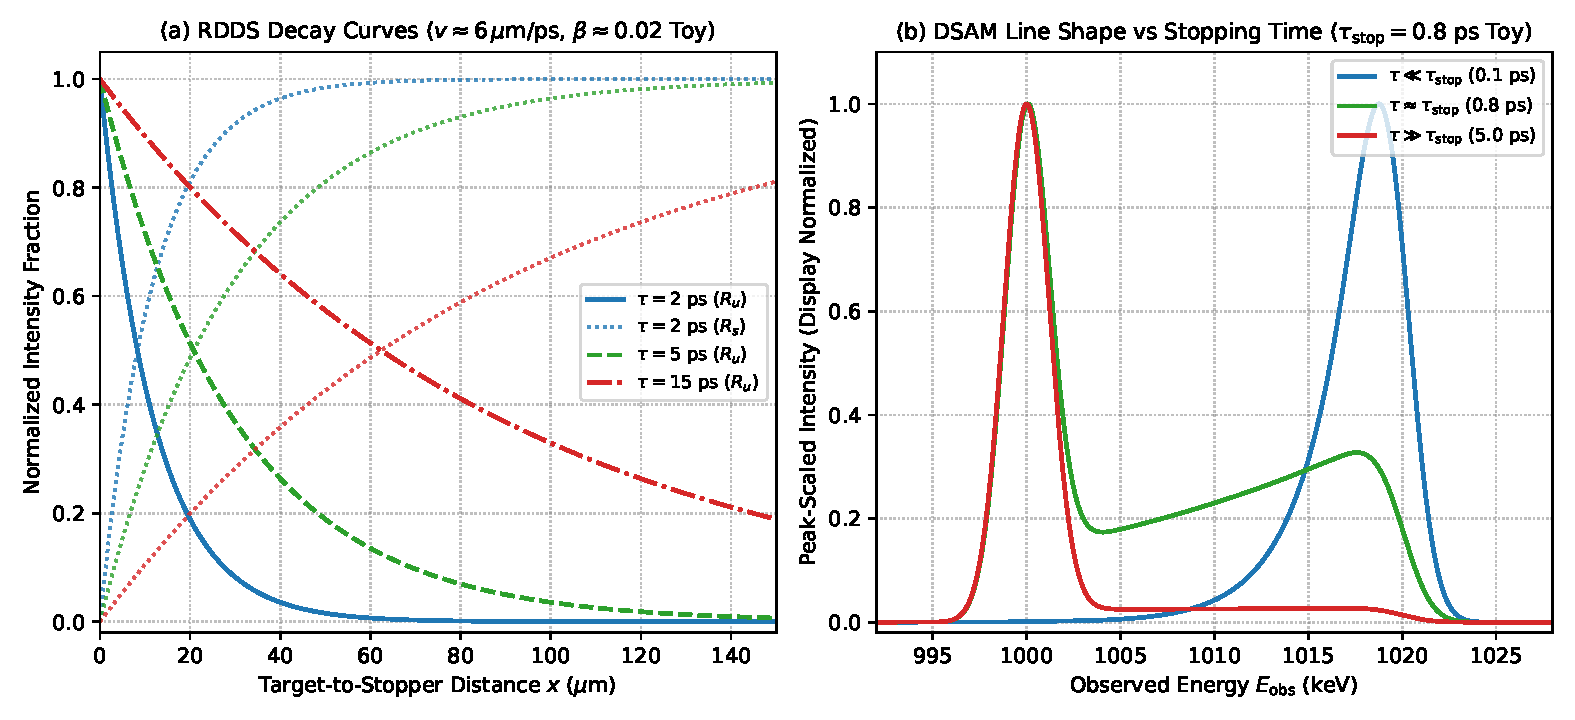
\includegraphics[width=0.98\textwidth]{Img/lifetime-response-rdds-dsam.pdf}
\caption[核态寿命测量物理响应模型对比]{核态寿命测量物理响应模型对比（规范教学示例）。(a) 展示反冲速度 $v \approx 6.0\,\mu\mathrm{m/ps}$（对应 $\beta \approx 0.02$）时，RDDS 柱塞法静止峰份额 $R_u(x)$（实线代表 $\tau = 2\text{ ps}$、虚线代表 $5\text{ ps}$、点划线代表 $15\text{ ps}$）与飞行峰份额 $R_s(x)$（点线）随靶--阻止箔距离 $x$ 的演化规律；(b) 展示厚衬底中反冲核在减速时间 $\tau_{\mathrm{stop}} = 0.8\text{ ps}$ 教学模型下的 DSAM 多普勒谱形演化：超短寿命（$\tau \ll \tau_{\mathrm{stop}}$）表现为全频移峰，中间寿命（$\tau \approx \tau_{\mathrm{stop}}$）形成连续展宽拖尾线形，超长寿命（$\tau \gg \tau_{\mathrm{stop}}$）退化为全停滞峰。计算采用解析 bin 概率与连续网格高斯卷积，在所列网格与支持域上检查总发射概率、解析质心及谱形收敛，显示图线仅将各线形峰高缩放至 1.0 以便视觉比对形态。注意此处为规范教学模型，不作为特定实验测量的修正因子。}\label{fig:5-8-lifetime-response}
\end{figure}

图~\ref{fig:5-8-lifetime-response} 阐明了核态寿命测量的敏感窗口与极限判定准则：
\begin{enumerate}
\item \textbf{DSAM 的敏感窗口与极限}：
DSAM 的测时灵敏度由核态寿命与反冲核在衬底中的慢化减速时间尺度共同决定。若核态寿命远短于离子减速至产生可辨识频移的时间，绝大多数光子将在初始高速度下发射，退化为未减速全多普勒频移峰，此时实验仅能给出寿命上限；反之，若核态寿命显著长于离子完全停滞的时间，绝大多数原子核在减速停止后才退激，主要表现为静止单色峰，此时仅能给出寿命下限。处于中间过渡寿命区间的核态则形成兼具飞行展宽与停滞峰的连续多普勒线形，其实际测时敏感范围取决于探测器能量分辨率、几何探测角度与衬底阻止特性。
\item \textbf{RDDS 的敏感窗口与互补性}：
RDDS 依赖机械位移精度（对应飞行时间 $x/v$ 从皮秒至纳秒范围）。它避免了厚衬底连续慢化谱形对微观阻止截面复杂模型的强敏感依赖，在皮秒能区与 DSAM 形成测量互补；但需要注意，反冲核穿过有限厚度反应靶与阻挡箔表层时的微小能量损失与角度散射，在精密实验中仍须进行适当建模修正。
\item \textbf{电子学快定时的延伸}：
对于几十皮秒以上乃至微秒量级的较长寿命核态，第~5.4~节讨论的高性能探测器数字时间戳差分测量与符合时间谱指数衰减曲线拟合成为主导方案。
\end{enumerate}

在科学报告中，研究人员必须根据实际实验响应，如实给出确定寿命值或无敏感性上下限，绝不能将仪器极限或理论模型假设伪造成独立的高精度测定值。由 DSAM 与 RDDS 确定的自洽寿命参量，将直接输入第~5.9~节，用于反演微观电四极跃迁几率 $B(E2)$ 与磁偶极跃迁几率 $B(M1)$。
%
}{%
    \section{DSAM与RDDS的时间信息 [未完成]}\label{sec:5-8}%
    \textit{本节尚未完成。}%
}

%-- Section 5.9: 由$\tau$/branch/ICC到绝对EM
\setcounter{section}{8}%
\IfFileExists{Tex/Sections/sec-5-9.tex}{%
    \section{由寿命、分支与内转换到绝对电磁强度}\label{sec:5-9}

在束 $\gamma$ 谱学实验中，探测器阵列记录的原始物理量是由晶体电荷收集形成的电压脉冲、数字化波形、时间戳以及重构的能谱峰面积与符合计数。通过反冲核在减速介质中的多普勒展宽线形拟合或不同飞行距离下的谱形变化，实验分析能够提取激发态的平均寿命，并测定各退激光子峰的相对强度。然而，低能核结构理论——无论是刚性转子模型、三轴粒子-转子耦合模型还是微观准粒子随机相位近似——所直接计算并用于检验波函数结构的核心物理量，却是特定电磁多极辐射算符在初末态之间的约化跃迁几率 $B(XL)$。约化跃迁几率提供了初末态波函数在不可约球张量算符作用下的微观矩阵元模平方；若要进一步推断原子核的内禀电四极矩 $Q_0$、电荷四极形变参数 $(\beta, \gamma)$ 以及集体激发模式的微观性质，还需要借助于具体的几何映射或微观自洽结构模型。

由宏观谱学计数反演微观绝对电磁跃迁几率，构成了连接实验观测与理论模型的关键纽带。这一反演链条受到退激通道完备性假设、内转换电子竞争、多极混合几率振幅干涉定相，以及谱学分析中实验不确定度传播的制约。本节旨在建立一套由能级寿命观测量、通道分支比、内转换系数及多极混合比反演绝对约化电磁跃迁几率 $B(XL)$ 的因果链，明确各项物理量的定义、量纲换算及适用边界。

\subsection{母态衰变时间尺度与总衰变常数的确定}\label{subsec:5-9-1}

考虑激发能级上的母核量子态 $|i\rangle$。若将其退激视为单一能级的自发衰变过程，在无外场驱动下其未衰变核数服从指数衰变定律 $N(t) = N(0) e^{-\lambda_{\text{tot}} t}$。表征能级总衰变速率的物理量为母态总衰变常数 $\lambda_{\text{tot}}$，量纲为时间倒数（常用单位为 $\text{s}^{-1}$ 或 $\text{ps}^{-1}$）。

在实验谱学中，时间观测量通常以平均寿命或半衰期两种形式报告：
\begin{enumerate}
\item 平均寿命 $\tau$：定义为原子核处于该激发态存活时间的统计平均值：
\begin{equation}\label{eq:5-9-tau}
\tau \equiv \frac{\int_0^\infty t e^{-\lambda_{\text{tot}} t} dt}{\int_0^\infty e^{-\lambda_{\text{tot}} t} dt} = \frac{1}{\lambda_{\text{tot}}}.
\end{equation}
在多普勒频移衰减法（DSAM）与反冲距离多普勒频移法（RDDS）中，实验并非直接测量皮秒或飞秒的时间衰变曲线，而是通过减速介质中的反冲速度历史模型或靶-阻止箔距离依赖的谱形拟合提取平均寿命 $\tau$。
\item 半衰期 $T_{1/2}$：定义为未衰变核数减少至一半所需的时间间隔：
\begin{equation}\label{eq:5-9-thalf}
T_{1/2} = \tau \ln 2 \approx 0.69315\,\tau.
\end{equation}
在电子学延时符合法或放射性衰变链测量中，实验常直接报告半衰期 $T_{1/2}$。若原始输入为 $T_{1/2}$，代入衰变率计算时需使用 $\lambda_{\text{tot}} = \frac{\ln 2}{T_{1/2}}$。若在应当使用平均寿命 $\tau$ 的公式中误代入半衰期 $T_{1/2}$，计算得到的衰变常数将被偏高评估 $1/\ln 2 \approx 1.443$ 倍（增大微观跃迁率约 $44.3\%$）；反之，若在需要半衰期处误代入平均寿命，则会偏低评估 $\ln 2 \approx 0.693$ 倍（偏小约 $30.7\%$）。必须依据实验给出的明确时间量选用相应的换算关系。
\end{enumerate}

在共振散射或反应截面测量中，不稳定激发态表现为具有有限能量宽度的 Breit-Wigner 共振峰，其总能级宽度 $\Gamma_{\text{tot}}$ 与衰变常数满足：
\begin{equation}\label{eq:5-9-gamma-tot}
\Gamma_{\text{tot}} = \hbar \lambda_{\text{tot}} = \frac{\hbar}{\tau}.
\end{equation}
若实验测得的是能级宽度 $\Gamma_{\text{tot}}$（能量量纲，如 $\text{eV}$），代入跃迁率公式前，需首先除以约化普朗克常数 $\hbar$ 以得到总跃迁率：
\begin{equation}\label{eq:5-9-gamma-to-lambda}
\lambda_{\text{tot}} = \frac{\Gamma_{\text{tot}}}{\hbar}.
\end{equation}
当已知测量量为平均寿命 $\tau$ 时，总跃迁率直接由 $\lambda_{\text{tot}} = 1/\tau$ 给出。在后续基于带量纲实用跃迁率系数（如电四极跃迁常数 $C_{E2}$）的计算体系中，该实用常数内部已经包含了普朗克常数 $\hbar$ 与真空介电常数等基本物理量。在采用带量纲实用率常数进行反演时，不能在此数值上再次乘除 $\hbar$ 或 $\ln 2$，否则会导致量纲混淆与数值偏差。

\subsection{通道分支比与内转换竞争：总衰变率向光子率的解耦}\label{subsec:5-9-2}

母核激发态 $|i\rangle$ 通常存在多个平行的下行退激途径。由独立衰变几率的可加性，母态总衰变率等于所有独立出射通道衰变率之和：
\begin{equation}\label{eq:5-9-lambda-sum}
\lambda_{\text{tot}} = \sum_k \lambda_k.
\end{equation}
对于连接特定末态 $|f_k\rangle$ 的电磁跃迁支路 $k$，其通道衰变率可分解为发射纯光子的跃迁率 $\lambda_{\gamma, k}$ 与激发核外壳层电子的内转换（IC）跃迁率 $\lambda_{e, k}$ 之和：
\begin{equation}\label{eq:5-9-lambda-branch}
\lambda_k = \lambda_{\gamma, k} + \lambda_{e, k}.
\end{equation}
定义该跃迁的总内转换系数（ICC）为电子发射几率与光子发射几率之比：
\begin{equation}\label{eq:5-9-icc-def}
\alpha_k \equiv \frac{\lambda_{e, k}}{\lambda_{\gamma, k}}.
\end{equation}
利用内转换系数，通道总退激率可表征为光子发射率的倍数：
\begin{equation}\label{eq:5-9-lambda-k-icc}
\lambda_k = \lambda_{\gamma, k}(1 + \alpha_k).
\end{equation}

在谱学文献中，对分支比的讨论涉及总跃迁分支比、偏光子分支比与相对光子强度：
\begin{enumerate}
\item 总跃迁分支比 $b_k$：定义为该跃迁通道的总衰变率（光子与内转换电子之和）占母态总衰变率的物理份额：
\begin{equation}\label{eq:5-9-bk}
b_k \equiv \frac{\lambda_k}{\lambda_{\text{tot}}} = \frac{\lambda_{\gamma, k}(1 + \alpha_k)}{\lambda_{\text{tot}}}.
\end{equation}
在遍历全部退激通道的前提下，概率守恒要求 $\sum_k b_k = 1$。已知平均寿命 $\tau$ 与总分支比 $b_k$ 时，提取光子发射率的公式为：
\begin{equation}\label{eq:5-9-lambda-gamma-k}
\lambda_{\gamma, k} = \frac{b_k}{\tau (1 + \alpha_k)}.
\end{equation}
对应的偏光子半衰期为 $T_{1/2, k}^\gamma = \frac{(1 + \alpha_k) T_{1/2, \text{tot}}}{b_k}$。
\item 偏光子分支比 $b_{\gamma, k}$：定义为纯光子发射率占母态总衰变率的份额：
\begin{equation}\label{eq:5-9-b-gamma-k}
b_{\gamma, k} \equiv \frac{\lambda_{\gamma, k}}{\lambda_{\text{tot}}} = \frac{b_k}{1 + \alpha_k}.
\end{equation}
由此可见，只要存在内转换电子发射（$\alpha_k > 0$），各支路的偏光子分支比求和便满足 $\sum_k b_{\gamma, k} \le 1$。当内转换过程显著时，纯光子分支之和必然小于 1，这反映了电子发射对退激流的分流。
\item 相对光子强度 $a_k$ 与重归一化条件：高纯锗探测器阵列记录的是光子事件。经探测效率 $\varepsilon(E_\gamma)$ 校正后，实验获得各条峰的相对光子强度 $a_k \propto N_{\gamma, k} \propto \lambda_{\gamma, k}$。若定义观测光子份额 $r_k \equiv a_k / \sum_j a_j$，该比值满足 $\sum_j r_j = 1$，仅表示通道 $k$ 占所观测到的光子总数的比例。由于其分母未计入内转换电子的贡献，此光子比例 $r_k$ 既不等于总分支比 $b_k$，也不等于偏光子分支比 $b_{\gamma, k}$。只有在满足以下通道闭合前提时，才能由相对光子强度结合已知内转换系数计算光子跃迁率：
\begin{itemize}
\item 母态的所有退激通道均已被探测到且无遗漏弱分支；
\item 不存在未被观测的纯电单极 $E0$ 内转换电子退激（例如四极形状共存核中的 $0_2^+ \to 0_1^+$ 跃迁完全禁戒单光子发射，或某些 $2_2^+ \to 2_1^+$ 跃迁中包含显著的单极穿入电子分量）；
\item 母态无未计入的中子、带电粒子或竞争性弱衰变；能量允许时还须另计内对产生等非光子通道。
\end{itemize}
\end{enumerate}

当上述完备性条件满足时，总衰变率可表达为各光子通道（计入各自内转换）的求和：
\begin{equation}\label{eq:5-9-lambda-tot-flux}
\lambda_{\text{tot}} = \sum_j \lambda_j = \sum_j \lambda_{\gamma, j} (1 + \alpha_j) = C \sum_j a_j (1 + \alpha_j).
\end{equation}
结合 $\lambda_{\text{tot}} = 1/\tau$，可导出由相对光子强度归一化的光子跃迁率：
\begin{equation}\label{eq:5-9-lambda-gamma-from-a}
\lambda_{\gamma, k} = \frac{a_k}{\tau \sum_j a_j (1 + \alpha_j)}.
\end{equation}
如果能级存在未测定的 $E0$ 内转换电子跃迁或未计入的粒子发射支路，上述分母求和必然漏项，导致分母偏小。强行仅对观测到的光子强度归一化会将遗漏通道的退激流分配给已知光子支路，从而高估 $\lambda_{\gamma, k}$，并在反演所得的 $B(XL)$ 中造成人为的虚假增强。在通道不闭合的复杂核区，应当通过独立的实验测量给出总分支比，而不能仅由光子强度强行求和归一。

\subsection{多极选择定则与多极混合比 $\delta$}\label{subsec:5-9-3}

电磁跃迁的选择定则由角动量守恒与宇称守恒决定。对于初态自旋宇称 $I_i^{\pi_i}$ 向末态 $I_f^{\pi_f}$ 的辐射跃迁，出射辐射场的多极阶数 $L$ 必须满足三角不等式：
\begin{equation}\label{eq:5-9-triangular}
|I_i - I_f| \le L \le I_i + I_f.
\end{equation}
同时，初末态宇称变化满足：
\begin{equation}\label{eq:5-9-parity-sel}
\pi_i \pi_f = (-1)^L \quad (\text{对于 } EL), \qquad \pi_i \pi_f = (-1)^{L-1} \quad (\text{对于 } ML).
\end{equation}
当三角条件与宇称均允许M1和E2，且二者矩阵元均非零时，出射场可包含二者的相干叠加。下文明确忽略更高多极；$\Delta I=0,\pm1$ 与同宇称仍须同时满足三角条件上界，不能用于0→0辐射。根据多极辐射规范~\cite{lange-kumar-hamilton-1982-multipole-admixtures}，实多极混合比 $\delta(E2/M1)$ 定义为电四极与磁偶极辐射场的光子发射几率振幅之比：
\begin{equation}\label{eq:5-9-delta-amp}
\delta(E2/M1) \equiv \frac{\text{Amp}(E2)}{\text{Amp}(M1)}.
\end{equation}
全立体角积分后不同多极辐射场的干涉项抵消，纯光子总跃迁率等于两分量之和：$\lambda_\gamma = \lambda_\gamma(M1) + \lambda_\gamma(E2)$。实多极混合比的平方（一般复振幅取模平方 $|\delta|^2$）等于纯 $E2$ 与纯 $M1$ 的光子发射率之比：
\begin{equation}\label{eq:5-9-delta-sq}
\delta^2 = \frac{\lambda_\gamma(E2)}{\lambda_\gamma(M1)}.
\end{equation}
多极混合比 $\delta$ 是出射光子场发射几率振幅之比，它不仅包含微观约化矩阵元，还内含了光子动量因子 $q = E_\gamma / (\hbar c)$ 与电磁耦合参数。当磁辐射算符采用国际单位制（SI）电荷型磁多极算符 $\mathcal{M}_S(M1) \equiv \mathcal{M}_\mu(M1)/c$（显式包含 $\mu_N/c$ 因子，矩阵元量纲为 $\mu_N/c$，即 $e\cdot\text{fm}$）单独定义时，混合比与约化矩阵元的关系表述为：
\begin{equation}\label{eq:5-9-delta-def}
\delta(E2/M1) = \frac{\sqrt{3}}{10} \frac{E_\gamma}{\hbar c} \frac{\langle I_f \| \mathcal{M}(E2) \| I_i \rangle}{\langle I_f \| \mathcal{M}_S(M1) \| I_i \rangle}.
\end{equation}
此时电荷型磁算符满足 $\mathcal{M}_S(M1) = \mathcal{M}_\mu(M1)/c$，其矩阵元量纲为 $\mu_N/c$（具有电荷乘长度量纲 $e\cdot\text{fm}$），与 $\mathcal{M}(E2)$（量纲 $e\cdot\text{fm}^2$）及动量因子 $q$（量纲 $\text{fm}^{-1}$）相配使得 $\delta$ 为无量纲纯数。若在常规采用磁矩型算符 $\mathcal{M}_\mu(M1)$（量纲 $\mu_N$）的约定下，分母相应补入 $1/c$ 因子（或等价地将光速 $c$ 移至分子与 $E_\gamma/\hbar$ 搭配），数值比值与相位约定保持完全自洽。$\delta$ 不能视作初末态裸约化矩阵元的简单无量纲相除。本书在发射过程选用 Krane--Steffen 混合比约定：式\eqref{eq:5-9-delta-def}中的矩阵元、算符相位和几何系数按同一约定配套。对于 Hamilton 的 $F_k$ 和其定义的 $\delta$，角分布混合项写为 $+2\delta F_k(LL')$；这与上述矩阵元比的约定一致。Lange 等~\cite{lange-kumar-hamilton-1982-multipole-admixtures}给出的发射约定中 $\delta_{\rm KS}=-\delta_{\rm RB}$，转换文献时还必须同步转换几何干涉系数并区分发射与吸收。已发表数据保留来源原有符号及其约定；只有核实来源约定并需要统一比较时才显式换算，$\delta^2$ 与由其确定的多极份额不受此符号变换影响。

在给定混合跃迁光子发射率 $\lambda_\gamma$ 下，电四极与磁偶极各自的光子发射份额由以下无量纲比例确定：
\begin{equation}\label{eq:5-9-multipole-frac}
f_{E2} = \frac{\delta^2}{1 + \delta^2}, \qquad f_{M1} = \frac{1}{1 + \delta^2}.
\end{equation}
分多极光子发射率分别为：
\begin{equation}\label{eq:5-9-lambda-multipole}
\lambda_\gamma(E2) = \lambda_\gamma \frac{\delta^2}{1 + \delta^2}, \qquad \lambda_\gamma(M1) = \lambda_\gamma \frac{1}{1 + \delta^2}.
\end{equation}
该跃迁出射的总内转换电子率为 $\lambda_e = \alpha(M1) \lambda_\gamma(M1) + \alpha(E2) \lambda_\gamma(E2)$，混合跃迁的有效内转换系数 $\alpha_{\text{mix}}$ 必须按相同的光子强度份额进行自洽加权：
\begin{equation}\label{eq:5-9-alpha-mix}
\alpha_{\text{mix}} = \frac{\alpha(M1) + \delta^2 \alpha(E2)}{1 + \delta^2}.
\end{equation}
在处理角分布与角关联测量时，不同的历史文献采用了不同的相位约定（如 Krane-Steffen 约定与 Rose-Brink 约定）。相位约定的转换取决于具体的发射级联与几何张量定义，可能引起角分布干涉几何系数与拟合实数 $\delta$ 的符号变化。但相位约定的改变属于表示选择，不影响物理观测量 $\delta^2$、光子强度份额以及绝对跃迁几率的数值。

\subsection{绝对约化跃迁几率 $B(XL)$ 的提取与量纲常数重建}\label{subsec:5-9-4}

设母能级初态为 $|i\rangle = |\xi_i, I_i, M_i\rangle$，末态为 $|f\rangle = |\xi_f, I_f, M_f\rangle$。在 Wigner-Eckart 定理标准约定下，对末态磁量子数及光子偏振求和、并对初态磁子能级等权平均后，退激过程的下行约化跃迁几率定义为~\cite{book-suhonen-from-nucleons-to-nucleus}：
\begin{equation}\label{eq:5-9-b-down}
B(XL; i \to f) \equiv \frac{1}{2I_i + 1} |\langle \xi_f I_f \| \mathcal{M}(XL) \| \xi_i I_i \rangle|^2.
\end{equation}
由张量算符的共轭置换关系，激发跃迁（上行）与衰变跃迁（下行）之间的统计权重倒易关系满足：
\begin{equation}\label{eq:5-9-wigner-eckart}
(2I_i + 1) B(XL; i \to f) = (2I_f + 1) B(XL; f \to i).
\end{equation}
例如偶偶核基态带中 $B(E2; 0^+ \to 2^+) = 5 B(E2; 2^+ \to 0^+)$。实验与理论比对时需确认跃迁方向，混淆上下行统计因子会引入 $(2I_f+1)/(2I_i+1)$ 倍的数值偏差。

时变微扰论 Fermi 黄金定则给出电多极跃迁率的标准形式~\cite{book-suhonen-from-nucleons-to-nucleus}：
\begin{equation}\label{eq:5-9-lambda-el}
\lambda_\gamma(E\lambda) = \frac{2}{\varepsilon_0 \hbar} \frac{\lambda + 1}{\lambda [(2\lambda + 1)!!]^2} \left(\frac{E_\gamma}{\hbar c}\right)^{2\lambda + 1} B(E\lambda).
\end{equation}
Suhonen 在其专著第 6 章利用常数 $\alpha \approx 1/137.04$ 与 $\hbar c \approx 197.33\,\text{MeV}\cdot\text{fm}$，将其化为实用数值式（原书 Eq.~6.14）：
\begin{equation}\label{eq:5-9-suhonen-e}
\lambda_\gamma(E\lambda) = 5.498 \times 10^{22} f(\lambda) \left(\frac{E_\gamma[\text{MeV}]}{197.33}\right)^{2\lambda + 1} B(E\lambda)[e^2\,\text{fm}^{2\lambda}]\,\text{s}^{-1},
\end{equation}
其中几何因子定义为 $f(\lambda) \equiv \frac{\lambda + 1}{\lambda [(2\lambda + 1)!!]^2}$。对于电四极跃迁（$\lambda = 2$），$f(2) = \frac{3}{2 \cdot 15^2} = \frac{1}{150}$。由教材印出常数精确重建电四极跃迁率系数：
\begin{equation}\label{eq:5-9-ce2}
C_{E2} = \frac{5.498 \times 10^{22}}{150 \times (197.33)^5} \approx 1.2250333078 \times 10^9\,\text{s}^{-1}\,\text{MeV}^{-5}\,(e^2\,\text{fm}^4)^{-1}.
\end{equation}
这是教材圆数重建的算术值，尾数不代表新的精密常数；下文通常取 $C_{E2} \approx 1.2250 \times 10^9$。由测量输入反演微观绝对 $B(E2)$ 的表达式为：
\begin{equation}\label{eq:5-9-be2-extracted}
B(E2) = \frac{\lambda_\gamma(E2)}{C_{E2} E_\gamma^5} = \frac{b_k \delta^2}{\tau (1 + \alpha_k)(1 + \delta^2) C_{E2} E_\gamma^5}.
\end{equation}
式中 $E_\gamma$ 以 $\text{MeV}$ 输入，$\tau$ 以 $\text{s}$ 输入，反演所得 $B(E2)$ 单位为 $e^2\,\text{fm}^4$。若采用宏观单位 $e^2\,\text{b}^2$（$1\,\text{b} = 100\,\text{fm}^2 \implies 1\,e^2\,\text{b}^2 = 10^4\,e^2\,\text{fm}^4$），数值需相应除以 $10^4$。该常数已完全内含真空电磁常数与 $\hbar$，使用该实用公式时不应重复乘除 $\hbar$ 或 $\ln 2$。

对于磁偶极跃迁，本节与第2.7节统一采用磁矩型算符 $\mathcal M_{\mu}(M1)$，其核磁子为 SI 量 $\mu_N=e\hbar/(2m_p)$，并记相应的约化跃迁几率为 $B_{\mu}(M1)$，单位为 $\mu_N^2$。Suhonen 的电荷型磁算符满足 $\mathcal M_{S}(M1)=\mathcal M_{\mu}(M1)/c$，故 $B_{S}(M1)=B_{\mu}(M1)/c^2$。但按各自单位表示的无量纲数值相同：
\begin{equation}
b_{M1}\equiv\frac{B_S(M1)}{(\mu_N/c)^2}=\frac{B_\mu(M1)}{\mu_N^2}.
\end{equation}
原书 Eq.~(6.14) 对 $\lambda=1$ 给出~\cite{book-suhonen-from-nucleons-to-nucleus}
\begin{equation}\label{eq:5-9-cm1}
\begin{aligned}
\lambda_\gamma(M1) &= C_{M1}\left(\frac{E_\gamma}{\mathrm{MeV}}\right)^3 b_{M1}, \\
C_{M1} &= \frac{6.080\times10^{20}(2/9)}{197.33^3}\,\mathrm{s}^{-1}\simeq 1.7584\times10^{13}\,\mathrm{s}^{-1}.
\end{aligned}
\end{equation}
因此，原书采用 $(\mu_N/c)^2$ 单位时的 $b_{M1}$ 可直接作为常规 $\mu_N^2$ 单位下的数值使用。由光子分量反演磁矩型约化跃迁几率，得
\begin{equation}\label{eq:5-9-bm1-extracted}
B_{\mu}(M1)=\mu_N^2\frac{\lambda_\gamma(M1)}{C_{M1}(E_\gamma/\mathrm{MeV})^3}
=\mu_N^2\frac{b_k}{\tau(1+\alpha_k)(1+\delta^2)C_{M1}(E_\gamma/\mathrm{MeV})^3}.
\end{equation}
高斯单位制中核磁子定义为 $e_{\mathrm G}\hbar/(2m_pc)$，其中电荷 $e_{\mathrm G}$ 亦须采用高斯单位；不可将该定义与 SI 电荷及带量纲的光速数值直接混用。比较文献时应先确认算符和所用核磁子，再比较以相应单位归一的数值。

\subsection{理想教学算例：阶梯退激模型的全流程计算}\label{subsec:5-9-5}

为建立清晰、可追溯且物理自洽的反演范例，在此给出一个具有两条竞争退激支路的规范教学算例，并对全流程关键物理量进行精确数值求解。

设某核能级包含母态 $|i\rangle$（自旋宇称为 $I_i^\pi = 4^+$），测得平均寿命 $\tau = 5.00\,\text{ps} = 5.00 \times 10^{-12}\,\text{s}$。该态仅存在两条相互竞争的下行退激 $\gamma$ 跃迁，且确证无粒子发射或竞争性 $E0$ 单极内转换：
\begin{itemize}
\item 通道 1（跃迁至 $3^+$ 态）：末态 $I_f^\pi = 3^+$，自旋变化 $\Delta I = 1$ 且宇称不变。根据角动量三角条件 $|4 - 3| \le L \le 4 + 3$，允许的多极阶数为 $L = 1, 2, \dots$。其中磁偶极 $M1$（$L=1$）与电四极 $E2$（$L=2$）均满足宇称守恒。虽然更高阶多极成分理论上也满足三角条件，但其贡献通常被严重压低；本算例假定二者均有贡献（混合跃迁）。设跃迁能量 $E_{\gamma, 1} = 0.800\,\text{MeV}$，相对光子强度 $a_1 = 100.0$，实多极混合比 $\delta_1 = +1.50$。设定虚拟内转换系数为 $\alpha_1(M1) = 3.00 \times 10^{-3}$，$\alpha_1(E2) = 1.50 \times 10^{-3}$。
\item 通道 2（跃迁至 $2^+$ 态）：末态 $I_f^\pi = 2^+$，自旋变化 $\Delta I = 2$ 且宇称不变。根据三角条件 $|4 - 2| \le L \le 4 + 2$，$L = 1$ 的偶极跃迁被严格禁戒。虽然理论上还允许 $M3, E4$ 等更高阶多极，但其辐射跃迁几率比低阶成分低若干数量级；本教学算例假定更高阶多极成分可以忽略，仅保留主导的 $E2$ 成分（$\delta_2 \to \infty$）。设跃迁能量 $E_{\gamma, 2} = 0.500\,\text{MeV}$，相对光子强度 $a_2 = 25.0$，设定虚拟内转换系数为 $\alpha_2(E2) = 5.00 \times 10^{-3}$。
\end{itemize}

下面执行五步反演计算：
\begin{enumerate}
\item 计算母态总衰变率：
由 $\lambda_{\text{tot}} = 1/\tau$，
\begin{equation}\label{eq:5-9-ped-tot}
\lambda_{\text{tot}} = \frac{1}{\tau} = \frac{1}{5.00 \times 10^{-12}\,\text{s}} = 2.00 \times 10^{11}\,\text{s}^{-1}.
\end{equation}

\item 混合份额与内转换系数加权：
对于通道 1，多极混合比 $\delta_1 = 1.50 \implies \delta_1^2 = 2.25$。多极光子份额为：
\begin{equation}\label{eq:5-9-ped-frac-1}
f_{E2, 1} = \frac{2.25}{1 + 2.25} = \frac{9}{13} \approx 0.692308, \qquad f_{M1, 1} = \frac{1}{3.25} = \frac{4}{13} \approx 0.307692.
\end{equation}
有效内转换系数按光子份额加权：
\begin{equation}\label{eq:5-9-ped-alpha-mix}
\alpha_{\text{mix}, 1} = \frac{3.00 \times 10^{-3} + 2.25 \times 1.50 \times 10^{-3}}{3.25} \approx 1.9615 \times 10^{-3}.
\end{equation}
通道 2 为纯 $E2$，$\alpha_2 = \alpha_2(E2) = 5.00 \times 10^{-3}$。

\item 重构总退激通量并求解分支比：
相对光子强度加权内转换的总通量分母为：
\begin{equation}\label{eq:5-9-ped-flux-sum}
\sum_j a_j (1 + \alpha_j) = 100.0 \times (1 + 0.0019615) + 25.0 \times (1 + 0.00500) = 125.32115.
\end{equation}
各通道的总物理分支比为：
$b_1 = 100.0 \times 1.0019615 / 125.32115 \approx 0.799515$；
$b_2 = 25.0 \times 1.00500 / 125.32115 \approx 0.200485$。
满足物理归一条件 $b_1 + b_2 = 1.000000$。
各通道偏光子分支比为：
$b_{\gamma, 1} = 100.0 / 125.32115 \approx 0.797950$；
$b_{\gamma, 2} = 25.0 / 125.32115 \approx 0.199488$。
偏光子分支比之和为 $0.797950 + 0.199488 = 0.997438 < 1$，明确体现了内转换电子带来的退激流损失。

\item 分多极光子发射率分解：
各通道光子发射率为：
\begin{equation}\label{eq:5-9-ped-lambda-gamma}
\lambda_{\gamma, 1} = \frac{b_{\gamma, 1}}{\tau} \approx 1.59590 \times 10^{11}\,\text{s}^{-1}, \qquad \lambda_{\gamma, 2} = \frac{b_{\gamma, 2}}{\tau} \approx 3.98975 \times 10^{10}\,\text{s}^{-1}.
\end{equation}
分解通道 1 的多极分量：
\begin{equation}\label{eq:5-9-ped-lambda-e2-1}
\lambda_{\gamma, 1}(E2) = \frac{9}{13} \times 1.59590 \times 10^{11}\,\text{s}^{-1} \approx 1.10485 \times 10^{11}\,\text{s}^{-1},
\end{equation}
\begin{equation}\label{eq:5-9-ped-lambda-m1-1}
\lambda_{\gamma, 1}(M1) = \frac{4}{13} \times 1.59590 \times 10^{11}\,\text{s}^{-1} \approx 4.91046 \times 10^{10}\,\text{s}^{-1}.
\end{equation}
通道 2 主导的 $E2$ 光子率为 $\lambda_{\gamma, 2}(E2) = \lambda_{\gamma, 2} \approx 3.98975 \times 10^{10}\,\text{s}^{-1}$。

\item 反演绝对约化电磁跃迁几率：
采用 Suhonen 教材印出常数精确重建的前因子，对于式\eqref{eq:5-9-ce2}为 $C_{E2} \approx 1.2250333078 \times 10^9\,\text{s}^{-1}\,\text{MeV}^{-5}\,(e^2\,\text{fm}^4)^{-1}$；对于能量和强度均先按各自单位归一的式\eqref{eq:5-9-cm1}，实用率常数统一为 $C_{M1} = 1.7583758801 \times 10^{13}\,\text{s}^{-1}$。
对通道 1（$4^+ \to 3^+$），$E_{\gamma, 1}^5 = (0.800)^5 = 0.32768\,\text{MeV}^5$：
\begin{equation}\label{eq:5-9-ped-be2-1}
B(E2; 4^+ \to 3^+) = \frac{1.10485 \times 10^{11}}{C_{E2} \times 0.32768} \approx 275.24\,e^2\,\text{fm}^4,
\end{equation}
计算值为 $275.2371\,e^2\,\text{fm}^4$，折合 $0.0275\,e^2\,\text{b}^2$。
磁偶极成分在 $E_{\gamma, 1}^3 = (0.800)^3 = 0.512\,\text{MeV}^3$ 下显式写为：
\begin{equation}\label{eq:5-9-ped-bm1-1}
B_\mu(M1; 4^+ \to 3^+) = \mu_N^2 \frac{4.91046 \times 10^{10}\,\text{s}^{-1}}{C_{M1} (0.800)^3} \approx 0.005454\,\mu_N^2,
\end{equation}
计算值为 $0.00545432\,\mu_N^2$。

对通道 2（$4^+ \to 2^+$），$E_{\gamma, 2}^5 = (0.500)^5 = 0.03125\,\text{MeV}^5$：
\begin{equation}\label{eq:5-9-ped-be2-2}
B(E2; 4^+ \to 2^+) = \frac{3.98975 \times 10^{10}}{C_{E2} \times 0.03125} \approx 1042.19\,e^2\,\text{fm}^4,
\end{equation}
计算值为 $1042.1919\,e^2\,\text{fm}^4$，折合 $0.1042\,e^2\,\text{b}^2$。
\end{enumerate}

\subsection{分支比值中的寿命消去与协方差传递}\label{subsec:5-9-6}

在检验集体模型预言时，研究常关注从同一个能级出射的两条分支的跃迁强度比。考察从同一母能级 $|i\rangle$ 出射的支路 $1$ 与 $2$，两支路光子发射率之比为：
\begin{equation}\label{eq:5-9-ratio-branch}
\frac{\lambda_{\gamma, 1}}{\lambda_{\gamma, 2}} = \frac{b_{\gamma, 1}}{b_{\gamma, 2}} = \frac{a_1}{a_2}.
\end{equation}
母态平均寿命 $\tau$ 在比值中作为公因子代数相消。纯四极跃迁强度之比可进一步表示为：
\begin{equation}\label{eq:5-9-ratio-be2}
\frac{B(E2; 1)}{B(E2; 2)} = \frac{\lambda_{\gamma, 1}(E2)}{\lambda_{\gamma, 2}(E2)} \left(\frac{E_{\gamma, 2}}{E_{\gamma, 1}}\right)^5 = \frac{a_1 \frac{\delta_1^2}{1 + \delta_1^2}}{a_2 \frac{\delta_2^2}{1 + \delta_2^2}} \left(\frac{E_{\gamma, 2}}{E_{\gamma, 1}}\right)^5.
\end{equation}
在上述教学算例中，该比值直接算得 $\frac{275.24}{1042.19} \approx 0.2641$。母态寿命的具体数值对该相对强度比值不产生影响。

然而，寿命 $\tau$ 的消去仅排除了该单一标量因子的测量不确定度，其余实验物理参数的不确定度依然存在：
\begin{enumerate}
\item 多极混合比 $\delta$ 的敏感性取决于其误差尺度与导数形式。四极份额对混合比的导数为 $df_{E2}/d\delta = 2\delta / (1+\delta^2)^2$，在 $|\delta| = 1/\sqrt{3} \approx 0.58$ 附近灵敏度最高，而在极大或极小 $|\delta|$ 区间该导数趋于平缓。对于磁偶极跃迁 $B(M1) \propto 1/(1+\delta^2)$，相对误差传播需结合 $\delta$ 的实际实验测量分布具体评估。
\item 相对光子强度之比 $a_1 / a_2$ 取决于探测器在两处能量点的相对探测效率。效率曲线的标定误差会直接传递至比值中。
\item 实验测得的 $a_1$ 与 $a_2$ 往往存在协方差。这种协方差既可能由密集重叠峰拟合时的解谱相关性带来负协方差，也可能由共同的效率刻度曲线、全谱归一化或吸收修正带来正协方差。协方差的正负取决于具体的实验谱形与分析过程，忽略协方差可能低估或高估最终比值的总误差。
\end{enumerate}

当比对属于不同母能级的跃迁时，各个能级的平均寿命属于独立参量，不发生代数相消。在 DSAM 寿命提取中，减速离子在衬底中的阻止本领模型构成了一类主要的系统误差源。如果不同激发态的反冲离子减速历程、速度区间或衰变时间窗口具有高度相似性，阻止本领的共同系统误差可能在比值中部分相消；但若各能级的衰变时段与速度灵敏度存在差异，这种系统偏置便无法完全消除。

在误差传播分析中，线性化公式 $V_y \approx J V_x J^T$ 仅是一阶 Taylor 展开近似。在由角分布或方向角关联反演多极混合比 $\delta$ 时，方程关于 $\delta$ 为二次有理式，似然函数或剖面似然（Profile Likelihood）常呈现双峰或长尾特征；若采用贝叶斯推断讨论后验分布，则必须显式声明先验分布的选择。在存在双峰或非对称似然时，强行采用局域高斯对称协方差会掩盖真实的置信区间与竞争解分支。

\subsection{典型实验剖析：$^{163}$Lu 实验中的寿命与跃迁强度反演}\label{subsec:5-9-7}

在奇 $A$ 核 $^{163}$Lu 中三轴超形变带（TSD）的研究中，A. Görgen 等人（2004）利用劳伦斯伯克利国家实验室（LBNL）的 Gammasphere 阵列开展了厚金衬底（$12\,\text{mg/cm}^2$）上的 DSAM 实验，通过反应 $^{123}\text{Sb}(^{44}\text{Ca}, 4n)^{163}\text{Lu}$ 测定了 TSD1 带 8 个能级与 TSD2 带 7 个能级的平均寿命 $\tau$~\cite{campaign-g07-gorgen-2004-163lu-quadrupole-moments}。

在反演带内与带间绝对跃迁几率 $B(E2)$ 和 $B(M1)$ 时，该工作采用了特定的实验数据整合方案：
\begin{enumerate}
\item 带间分支比的外源采用：在厚衬靶实验中，反冲核在减速过程中出射的光子形成多普勒展宽峰。TSD1 带内退激跃迁占主导，测得的寿命可直接换算为带内跃迁强度；而对于存在带间竞争退激的 TSD2 候选带，作者在论文中指出，由于厚靶展宽峰难以拟合弱带出分支，提取带间跃迁所需的带出分支比直接借用了先前薄靶实验（Jensen 等人 2002）的测量结果。
\item 多极混合比的平均值外推：为了将带间连接跃迁分解为 $B(E2)_{\text{out}}$ 与 $B(M1)_{\text{out}}$，作者在计算中采用了先前角关联实验在自旋 $I \le 51/2$ 态测得的平均混合比 $\delta = -3.10^{+0.36}_{-0.44}$，并假定该数值在整个自旋区间保持恒定。
\item 误差来源的标示：作者报告的误差主要源自 $\chi^2$ 拟合的协方差及不同角度的分散度，并未包含阻止本领模型选择所引入的全局系统不确定度。
\end{enumerate}

在物理诠释方面，Görgen 等人在其采用的摆动运动图像下，将 TSD1 与 TSD2 测得的相近跃迁四极矩 $Q_t$ 作为两带基于相同内禀结构的支持依据。需要说明的是，原文 Table~I 中报告的 $Q_t$ 数值在不同自旋态之间存在显著的分散范围；作者推算的两带间约 $4\%$ 的细微差异，也是基于其特定核心角动量倾角估计得到的理论数值。从谱学方法学的角度来看，观测到相似的跃迁四极矩及较强的带间退激与摆动模型相容，但这种电磁跃迁特征亦可能由准粒子在形变核芯中的对齐耦合、$\gamma$ 软核芯中的大振幅涨落或四极振动模式混合所产生。在确立微观结构解释时，必须将这些竞争性模型机制纳入综合考量。

由激发态寿命、分支比与内转换系数反演得到的约化电磁跃迁几率 $B(XL)$，在量子力学上直接给出了特定初末态波函数在多极辐射算符下的矩阵元模平方。然而，$B(XL)$ 本身并不等同于内禀几何形状参数；要将其进一步翻译为内禀四极矩、形状不对称角 $\gamma$ 或摆动激发等微观物理图像，还必须依赖具体的核结构理论模型。实验所提取的绝对跃迁强度与相对比值，将作为下一节（第~5.10~节）统计推断以及第~4~章集体运动动力学模型比对的关键输入。
%
}{%
    \section{由$\tau$/branch/ICC到绝对EM [未完成]}\label{sec:5-9}%
    \textit{本节尚未完成。}%
}

%-- Section 5.10: 统计推断与结果章接口
\setcounter{section}{9}%
\IfFileExists{Tex/Sections/sec-5-10.tex}{%
    \section{统计推断与实验结果接口}\label{sec:5-10}

在在束 $\gamma$ 谱学分析中，研究人员经历了探测器物理响应（第~5.2~节）、数字波形滤波（第~5.3~节）、高精度定时（第~5.4~节）、硬件活时间与符合选择（第~5.5~节）、符合矩阵与能级拓扑构建（第~5.6~节）、角分布与偏振反演（第~5.7~节）以及微观寿命测量（第~5.8~节）的全流程处理。最终，这些宏观测量必须被综合转化为原子核微观结构的确定物理量——能级激发能 $E_x$、自旋宇称 $I^\pi$、多极混合比 $\delta$、能级平均寿命 $\tau$ 以及绝对电磁约化跃迁几率 $B(XL)$。

然而，由离散计数直方图到连续物理参数的提取并非简单的代数代入，而是一个面临多重不确定度耦合的统计推断反问题。若在分析中机械套用高斯近似或简单忽略系统协方差，容易产生严重的推断失真：其一，在角分布二次反演产生多解双峰、或者微弱谱线处于物理非负边界（$B(XL) \ge 0$）附近时，盲目套用线性误差传播（$\mathbf{J} \mathbf{V} \mathbf{J}^T$）或标准渐近 Wilks 定理，会导致置信区间侵入非物理负值区，或者虚假排除相容解分支；其二，混淆不同测量通道的系统误差与统计涨落，在模型与实验存在微小偏离时轻率宣称发现了新物理。本节构建面向在束谱学的前向测量统计模型，阐明非独立计数似然与非线性协方差传递机制，深入剖析高斯正则性破缺下的轮廓似然与 Feldman-Cousins 物理边界区间构建方法，严格区分统计与系统误差的因果属性，并最终确立标准化的核结构实验结果数据接口。

\subsection{前向测量模型与非独立计数似然}\label{subsec:5-10-1}

在统计物理学中，严谨的实验推断应当建立在前向生成模型（Forward Measurement Model）的基础之上。设系统待求解的微观核结构物理参数集合为 $\boldsymbol{\theta}$（如各能级 $B(E2)$、$B(M1)$、寿命 $\tau$ 及混合比 $\delta$），影响观测但非直接研究目标的伴随扰动参数（Nuisance Parameters，如探测器绝对效率曲线拟合参数、偶然符合归一化因子 $a$、衬底停止本领经验修正因数及侧向馈入时间分布参数）集合记为 $\boldsymbol{\nu}$。

在束实验中，探测器阵列记录的原始能谱由离散事件累积而成。必须明确：离散分箱或事件级记录本身并不自动保证各能量仓计数服从相互独立的泊松分布。各通道计数服从条件独立泊松分布属于分箱近似模型，其物理前提要求满足单通道互斥分类或采用恰当的事件级似然；即使底层复合核反应可近似为泊松点过程，单次核退激仍可能同时发射多个级联光子（多重性 $M_\gamma > 1$），在未做符合拓扑分离时会在不同能量仓之间引入事件级相关。低的每束团反应概率本身不足以证明泊松过程，还需检查束流统计和事件独立性。固定总数并按互斥类别分类时可采用多项模型；硬件容量限制则可能引入停止规则、死时间或选择偏差，需按实际记录过程建模。此外，完整的实验联合似然函数不仅包含信号与连续本底能谱的计数似然，还可纳入来自带外平坦区的背景控制样本以及辅助测量约束。当各辅助标定测量相互条件独立时，辅助项可写作独立概率密度之积；若辅助测量本身存在相关性，则须采用联合概率密度 $p_{\mathrm{aux}}(\mathbf{a} \mid \boldsymbol{\nu})$~\cite{book-zhu-probability-statistics-in-physics, book-behnke-data-analysis-hep, baker-cousins-1984-histogram-fits}：
\begin{equation}\label{eq:5-10-poisson-likelihood}
\mathcal{L}(\boldsymbol{\theta}, \boldsymbol{\nu} \mid \mathbf{n}, \mathbf{a}) = \left[ \prod_{k=1}^K \frac{\mu_k(\boldsymbol{\theta}, \boldsymbol{\nu})^{n_k} e^{-\mu_k(\boldsymbol{\theta}, \boldsymbol{\nu})}}{n_k!} \right] \times p_{\mathrm{aux}}(\mathbf{a} \mid \boldsymbol{\nu}),
\end{equation}
其中 $\mu_k(\boldsymbol{\theta}, \boldsymbol{\nu}) = Y_{\gamma, k}(\boldsymbol{\theta}, \boldsymbol{\nu}) + B_k(\boldsymbol{\nu})$ 为第 $k$ 仓的理论预期计数，$\mathbf{a}$ 为辅助标定观测量，$p_{\mathrm{aux}}(\mathbf{a} \mid \boldsymbol{\nu})$ 为其对应的辅助测量联合概率密度。

前向生成模型式~\eqref{eq:5-10-poisson-likelihood} 明确了从微观物理参数到宏观计数的因果正向映射。与传统启发式峰面积提取相比，它具有以下特性：
\begin{enumerate}
\item 统一表征共享扰动参数引入的相关性：
当不同能量的峰共处于同一测量体系中时，它们对某些全局参数（如总探测时间、绝对效率刻度或探测器死时间因子）的依赖具有强关联。联合似然将这些共性因子作为共享扰动参数 $\boldsymbol{\nu}$ 统一处理，能够定量描述由参数不确定度诱导的协方差；而对多光子事件聚类等底层物理相关性，则需进一步通过事件级联合似然或符合矩阵模型单独表征。
\item 比值中心值丢弃了原始似然形状：
在实验文献中，常将测量结果压缩报告为单峰面积比值（如相对光子强度比或 DCO 强度比）。仅凭比值的中心值与一阶对称误差，无法还原多维空间中由于泊松涨落与效率非线性传递引起的非对称似然曲面。
\end{enumerate}

\subsection{非线性误差传递、Jacobian矩阵与协方差网络}\label{subsec:5-10-2}

当从中间实验观测向量 $\mathbf{x}$（如净峰面积 $A_\gamma$、门选比值、寿命 $\tau$、转换系数 $\alpha_{\mathrm{IC}}$）向最终物理参数向量 $\mathbf{y} = \mathbf{g}(\mathbf{x})$（如绝对 $B(E2)$ 几率）转换时，普遍采用基于一阶 Taylor 展开的线性化误差传播：
\begin{equation}\label{eq:5-10-covariance-prop}
\mathbf{V}_y \approx \mathbf{J} \mathbf{V}_x \mathbf{J}^T,
\end{equation}
其中 $\mathbf{J}$ 为函数的一阶偏导数 Jacobian 矩阵，元素满足 $J_{ik} = \frac{\partial g_i}{\partial x_k}$，$\mathbf{V}_x$ 为输入参量的协方差矩阵。对任一标量输出物理量 $y_i$，其总方差展开式为：
\begin{equation}\label{eq:5-10-var-sum}
\sigma_{y_i}^2 \approx \sum_k J_{ik}^2 \sigma_{x_k}^2 + 2 \sum_{k < l} J_{ik} J_{il} \mathrm{Cov}(x_k, x_l).
\end{equation}

在核物理反演实践中，必须严格审查式~\eqref{eq:5-10-var-sum} 的适用边界（朱永生 2006 第 3 章 §3.9，印刷第 67--70 页，PDF 第 83--86 页~\cite{book-zhu-probability-statistics-in-physics}; Bonamente 2022 第 5 章 §5.2，印刷第 83--87 页，PDF 第 103--107 页，例 5.3~\cite{book-bonamente-statistics-scientific-data}）：
\begin{itemize}
\item 必须保留非零协方差项：
在一阶展开下，当输入参量 $x_k$ 与 $x_l$ 统计不相关（即协方差 $\mathrm{Cov}(x_k, x_l) = 0$）或交叉项代数相消时，总方差才退化为简单的对角平方和 $\sigma_{y_i}^2 = \sum_k J_{ik}^2 \sigma_k^2$。必须明确：不相关性（协方差为零）弱于统计独立性；协方差为零并不自动意味着输入变量相互独立，但在关于均值的一阶 Taylor 展开中，不相关性已足以使交叉协方差项在方差求和中消失。
在在束谱学中，必须清晰区分原始解谱净峰面积 $A_i$（计数）与经效率及活时间校正后的跃迁强度 $I_i = A_i / (\varepsilon(E_i) \cdot \mathrm{LT})$：其中 $\mathrm{LT} \in (0, 1]$ 为无量纲的单探测器活时间份额（Live-Time Fraction），该因式分解假定了探测效率与活时间测量相互独立且信号无时间相关丢失；当处理多探测器符合测量时，正如第~5.5~节所述，联合符合接受度受通道间死时间相关性约束，不能简单拆解为各单道独立效率与活时间的标量积。原始峰面积的拟合协方差 $\mathbf{V}_A$ 源自多高斯解谱或背景扣除（紧密重叠峰通常呈现负相关，但复杂的共同连续本底可能改变相关符号；远离孤立峰近乎零相关）；而经校正后的跃迁强度 $I_i$ 则额外引入了共享探测效率曲线拟合参数的协方差传递。共享全局效率参数在不同能量区间可能引入正协方差或负协方差（取决于效率参数化曲线的局域斜率与曲率），不能笼统假定所有通道间协方差必为正，亦不能在非多项分布情形下断言分支协方差必为负。无声明地丢弃协方差项会严重歪曲最终跃迁几率的总不确定度。
\item 非线性强曲率与代入估计量界限：
对于非线性映射 $\mathbf{g}(\mathbf{x})$，式~\eqref{eq:5-10-covariance-prop} 仅是一阶线性近似。正如第~5.6~节所指出的，对于净计数 $S = P - aR$，在固定 $a$ 与独立泊松条件下理论总体方差为 $\mathrm{Var}(S) = \mu_P + a^2 \mu_R$, 而实验计算中的 $P + a^2 R$ 属于样本代入估计量 $\widehat{\mathrm{Var}}(S)$。当函数具有强非线性曲率（如 $B(E2) \propto E_\gamma^{-5} \tau^{-1}$ 且相对误差较大时），一阶高斯展开可能不足以描述均值、方差或尾部。当解析误差传播由于高度非线性或多峰结构失效时，可以通过对输入物理量的联合分布进行蒙特卡罗抽样，将样本代入非线性转换模型 $\mathbf{g}(\mathbf{x})$ 得到输出参数的前向推演分布（Pushforward Distribution）。必须明确：这种前向抽样反映的是测量误差在外推变换下的统计传播，仅当输入样本本身已经直接来自于相应的条件后验分布时，输出样本的经验直方图才构成合法的参数后验分布；仅仅在输入端形式化附加一个先验分布并不足以使前向抽样等同于严密的贝叶斯后验推断。
\end{itemize}

\subsection{高斯正则性破缺：多峰似然、物理边界与Feldman-Cousins构建}\label{subsec:5-10-3}

传统统计学常假定参数估计量渐近服从正态高斯分布。渐近 Wilks 定理（Wilks 1938; 朱永生 2006 第 12 章 §12.2.2，印刷第 394--398 页，PDF 第 410--414 页~\cite{book-zhu-probability-statistics-in-physics}; Behnke 等 2013 第 2 章 §2.3，印刷第 37--38 页，PDF 第 55 页~\cite{book-behnke-data-analysis-hep}）指出：在零假设处于参数空间内部（无边界效应）且大样本正则条件成立的极限下，对 $m$ 个感兴趣物理参数（Parameters of Interest）进行检验的轮廓似然比统计量 $-2\Delta\ln\lambda(\boldsymbol{\theta})$ 渐近服从自由度等于 $m$ 的 $\chi^2$ 分布，即自由度仅由被检验的物理参数维数 $m = \dim(\boldsymbol{\theta})$ 决定，而不包含被剖面优化消除的伴随扰动参数（Nuisance Parameters）维数。对于单参数检验（$m=1$），双侧 $1\sigma$ 对应 $\Delta\chi^2 = 1.0$，双侧 $95\%$ 置信度对应 $\Delta\chi^2 = 3.84$。
在内部正则点和选定分支的局部高斯近似中，曲率可用于估计协方差。下式中的目标函数应已对伴随参数作剖面优化；也可以先对完整自由参数求Hessian并取其逆矩阵中的相应协方差子块。必须明确 Hessian 矩阵的目标函数定义：若采用负对数似然函数 $F_1(\boldsymbol{\theta}) = -\ln\mathcal{L}$，其二阶导数矩阵（观测 Fisher 信息阵）为 $\mathbf{H}_1 = \nabla^2(-\ln\mathcal{L})$，协方差矩阵近似为 $\mathbf{V}_{\boldsymbol{\theta}} \approx \mathbf{H}_1^{-1}$；若采用检验统计量形式 $F_2(\boldsymbol{\theta}) = -2\ln\mathcal{L}$，其 Hessian 矩阵为 $\mathbf{H}_2 = \nabla^2(-2\ln\mathcal{L}) = 2\mathbf{H}_1$，对应的协方差矩阵近似为 $\mathbf{V}_{\boldsymbol{\theta}} \approx 2 \mathbf{H}_2^{-1}$，推导与编程实现中不可遗漏系数 2。若伴随参数已被轮廓极小化消除，二阶导数反映的是轮廓曲率（Profile Curvature）。
同时必须注意：轮廓似然曲线本身并不自动产生具备精确置信覆盖的置信区间。轮廓似然比区间的置信水平保证依赖于其渐近卡方极限；在有限小样本、多峰或边界附近，精确的置信覆盖必须依赖于对参考分布的构建，例如通过严格的 Neyman 接受带构造、小样本下的离散精确枚举或蒙特卡罗校准获取经验参考分布。在真实的在束核谱学分析中，高斯正则性条件（Gaussian Regularity）常面临以下物理局限：
\begin{enumerate}
\item 多极混合比 $\delta$ 反演的双根多解（Multi-Root Degeneracy）：
在角分布 $W(\theta)$ 或 DCO 强度比的二次有理拟合中，由于二次方程的代数结构，似然曲面常呈现两个分离的极小值峡谷（见图~\ref{fig:5-10-inference-profile}(a)）。在每一个局部极小值附近，局域二阶导数展开（轮廓曲率）可以给出该分支内的局域有效误差；但在全局统计推断中，必须完整报告相容的两个孤立解分支，不能将多峰曲面强行用单高斯抛物线拟合，更不能随意丢弃第二解分支。
\item 物理边界截断与 Feldman-Cousins 统一方法：
核跃迁辐射几率具有严格的物理非负边界（如 $B(E2) \ge 0$、寿命 $\tau \ge 0$）。当微弱谱线由于本底统计下涨落导致无约束极大似然估计量出现负值（$\widehat{\mu} < 0$）时，标准双侧高斯置信区间会导致区间侵入非物理负值区与物理域取交集后还可能得到空集；而若实验人员事后根据估计值正负自行决定报告单边上限还是双边区间（Flip-Flopping），会导致真实的覆盖率严重低于名义置信水平（Undercoverage）。
一种预先固定似然比排序、避免事后翻转报告规则的方法是 Feldman-Cousins 统一方法（Feldman \& Cousins 1998; 朱永生 2006 专著第 11 章 §11.2 似然比顺序求和方法，印刷第 377--379 页，PDF 第 393--395 页，式 (11.2.2)--(11.2.4)~\cite{book-zhu-probability-statistics-in-physics}; Behnke 等 2013 专著第 4 章 §4.3，印刷第 122--123 页，PDF 第 138--139 页 Table 4.2~\cite{book-behnke-data-analysis-hep}）：该方法基于广义似然比排序原理 $R(n \mid \mu) = P(n \mid \mu) / P(n \mid \hat{\mu}_{\mathrm{phys}})$（其中 $\hat{\mu}_{\mathrm{phys}} = \max(0, \hat{\mu})$ 为物理受限极大似然估计），对声明的生成模型（如已知本底 $b$ 下的泊松信号）在参数空间上逐点构造 Neyman 接受带并进行反演。必须明确：对于离散泊松计数，接受带的端点随整数计数跳跃变化，通常表现出保守的阶梯状过覆盖（Over-coverage）；Feldman-Cousins 方法绝非简单在连续轮廓似然曲线上截取 $\Delta\chi^2 = 2.71$（后者仅为一维渐近单侧 $95\%$ 正态标尺，见图~\ref{fig:5-10-inference-profile}(b) 展示），更不能在任意包含复杂伴随参数剖面优化的情形下假定普适平滑覆盖。当报告置信区间与上限时，必须明确声明所选取的推断构型、置信水平、排序准则以及伴随参数的处理流程。
\end{enumerate}

为直观展示上述高斯破缺机制及规范统计处理方法，图~\ref{fig:5-10-inference-profile} 给出了基于标准教学模型的合成多峰剖面与同一高斯观测下的受限似然对比图。

\begin{figure}[!htbp]
\centering
%
  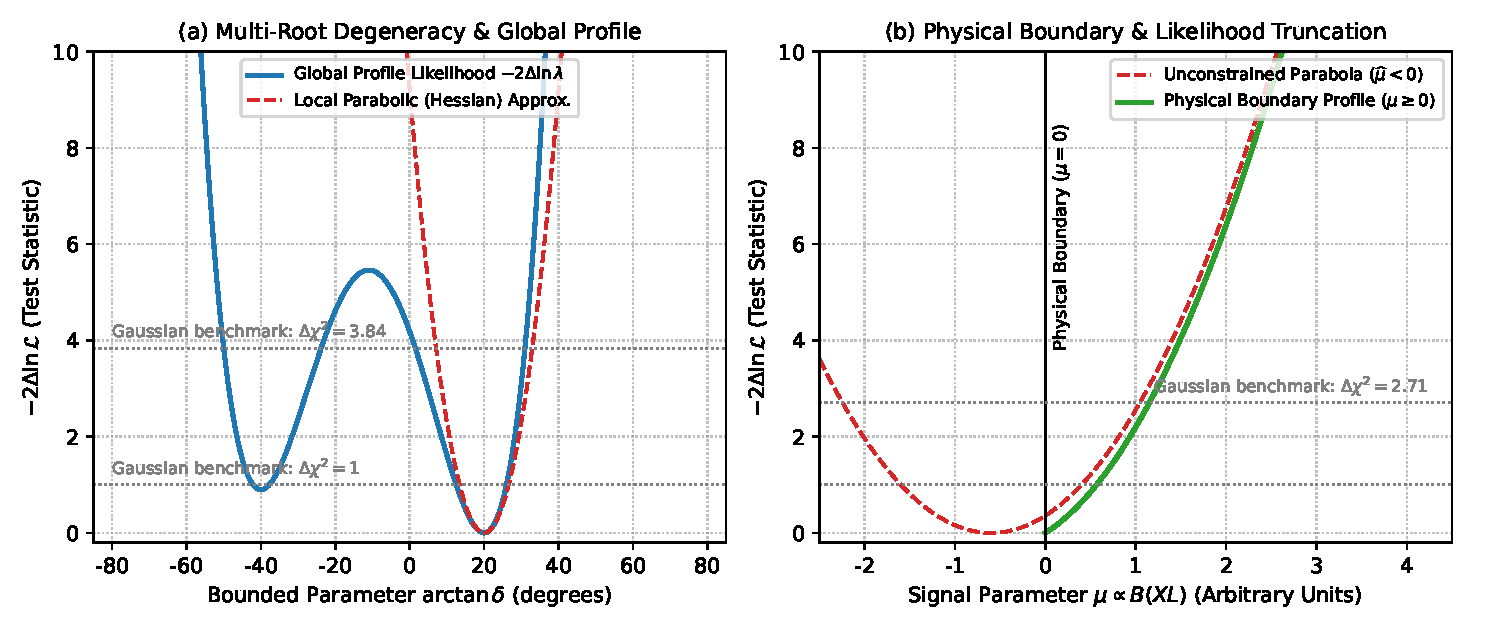
\includegraphics[width=0.92\textwidth]{Img/inference-profile-likelihood-boundary.pdf}%
\caption[核谱学高斯正则性破缺与统计推断模型对比]{核谱学高斯正则性破缺与统计推断模型对比（规范教学模型）。(a) 展示多极混合比 $\delta$ 在有界坐标 $\arctan\delta$ 上的整体轮廓似然曲线（实线），呈现清晰的双极小值结构；虚线是该合成函数在右侧极小点处的实际二阶Taylor近似，说明对称高斯假设完全丢弃了第二解分支；(b) 展示信号参数处于物理非负边界（$\mu \ge 0$）时的轮廓似然曲线：虚线为允许负值的无约束剖面（极小值处于统计负涨落点 $\widehat{\mu} < 0$），绿色实线展示了严格定义在物理非负定义域 $\mu \ge 0$ 上且归一至受限极大值 $\hat{\mu}_{\mathrm{phys}} = 0$ 的轮廓似然剖面，受限曲线由同一观测 $\widehat\mu=-0.6$ 的高斯对数似然减去其物理最优点处的值构成；约束只改变参考极大值，不将观测均值重置为零（图中1、3.84与2.71水平均仅作一参数高斯标尺，未给该合成多峰例校准覆盖率；$\Delta\chi^2 = 2.71$ 虚线仅表示一维高斯渐近单侧 $95\%$ 标尺，不代表通用的 Feldman-Cousins 覆盖结果；严格的 Feldman-Cousins 统一区间构建基于对具体生成模型的似然比排序 Neyman 接受带反演，离散泊松计数呈现阶梯状过覆盖，不可直接等同于连续曲线截断）。注意此处为规范教学模型展示，非特定未知实验测量拟合）。}
\label{fig:5-10-inference-profile}
\end{figure}

针对图~\ref{fig:5-10-inference-profile} 所示的非正则场景，在数据分析中应规范应用以下推断方法：
\begin{itemize}
\item 轮廓似然方法（Profile Likelihood）：
对于包含众多扰动参数 $\boldsymbol{\nu}$ 的复杂模型，通过在固定感兴趣物理参数 $\boldsymbol{\theta}$ 的条件下对所有扰动参数进行受限极大似然优化（$\hat{\hat{\boldsymbol{\nu}}}(\boldsymbol{\theta})$），构建单变量或双变量的轮廓似然比检验统计量：
\begin{equation}\label{eq:5-10-profile-likelihood}
\lambda(\boldsymbol{\theta}) \equiv \frac{\mathcal{L}(\boldsymbol{\theta}, \hat{\hat{\boldsymbol{\nu}}}(\boldsymbol{\theta}))}{\mathcal{L}(\hat{\boldsymbol{\theta}}, \hat{\boldsymbol{\nu}})}.
\end{equation}
轮廓似然方法自动将扰动参数的统计不确定度沿极小化路径向外投影，从而在输出曲线上产生反映非线性与关联效应的非对称置信区间。必须注意：仅当样本量充足且处于内部正则区时，$-2\ln\lambda(\boldsymbol{\theta})$ 才渐近服从自由度为 $\dim(\boldsymbol{\theta})$ 的 $\chi^2$ 分布；在小样本或边界情形下，必须结合蒙特卡罗校准获取经验参考分布。
\item 蒙特卡罗抽样与推演分布（Monte Carlo Pushforward）：
当解析误差传播由于高度非线性或多峰结构失效时，可以通过对输入物理量的联合分布进行蒙特卡罗大样本抽样，将样本代入非线性转换模型 $\mathbf{g}(\mathbf{x})$ 得到输出参数的前向推演分布。必须明确：这种前向抽样反映的是测量误差的传播分布，仅当输入样本本身已经直接来自于相应的条件后验分布时，输出分布方可作为贝叶斯后验概率密度解释。
\end{itemize}

\subsection{系统误差、统计涨落与模型假象的甄别}\label{subsec:5-10-4}

在科学写作与理论比对中，必须严格区分两类性质根本不同的实验不确定度来源：
\begin{enumerate}
\item 统计涨落误差（Statistical Uncertainty）：
源于核衰变发射与探测器电荷电离过程的本征微观量子随机性。在渐近独立平稳泊松极限下，计数的绝对统计标准差按 $\sigma \sim \sqrt{N_{\mathrm{counts}}}$ 增长，而相对统计精度按 $1/\sqrt{N_{\mathrm{counts}}}$ 改善；通过延长束流照射时间可以在统计涨落层面提高信噪比。
\item 系统不确定度（Systematic Uncertainty）：
源于物理模型假设偏差、仪器刻度基准偏移以及探测环境的全局畸变。系统不确定度并不必然在所有探测通道呈现相同方向，且不能通过简单延长机时来消除；部分系统偏差可通过增加辅助刻度实验予以缩小。在低能核物理在束谱学中，典型的系统误差来源包括：
\begin{itemize}
\item 探测器绝对全能峰效率曲线的参数化拟合不确定度及其跨能区协方差传递；
\item 第~5.8~节 DSAM 谱形拟合中所采用的固体衬底微观电子/核停止本领理论模型参数差异（如 SRIM 与 Northcliffe-Schilling 唯象参数之间的系统离散）；
\item 反应靶实际厚度、同位素纯度与反冲慢化介质密度的实验测量公差；
\item 符合时间窗口截断与偶然本底扣除归一化比例因子 $a$ 的拟合或标定不确定度。
\end{itemize}
\end{enumerate}

在核结构科学推断中，提出一项新的物理模式候选（如手征双重带或摆动激发候选），需要明确说明其实验指征、模型依赖性以及当前的观测边界；而确证一项新的集体模式主张，则必须对已知的仪器效应、数据处理假象以及常规竞争机制（如准粒子顺排带交叉、形状共存或 $\gamma$ 振动）开展系统的敏感性检验与排他性评估。研究人员应重点核查以下竞争性仪器与方法学因素：
\begin{enumerate}
\item 观察到的弱支路偏离是否完全处于探测器全能峰效率曲线与偶然相加校正的系统误差包络之内；
\item 提取的能级寿命是否受到了未被观测的慢速侧向馈入（Side-Feeding）或未知同核异能态的滞后卷积（见第~5.1~节与第~5.8~节）；
\item 角分布多极混合比反演中是否存在另一个完全相容的数学解分支尚未被排除（见第~5.7~节）；
\item 微观理论模型本身是否由于冻结了准粒子对齐、采用了单态平均场惯量参数或忽略了 $\gamma$ 自由度的大振幅涨落而导致模型自身预测失真。
\end{enumerate}
确证一项新的集体模式主张需要开展相称的排他性检验与系统敏感性核查；而探索性的物理模式候选则可以基于初步观测指征提出，并清晰声明其灵敏度边界与待验条件。

\subsection{核结构实验结果标准输出数据接口}\label{subsec:5-10-5}

为了将第 5 章所建立的在束谱学因果链条严密固化为可供理论模型（第 2、3、4 章）直接检验的高保真实验结果，本节确立了一套标准化的核结构实验输出数据接口。

在正式的学位论文与学术成果报告中，任何一条关于能级与电磁强度的陈述，均应在数据表中完整列出其初末态量子数、观测谱学量、中间修正因子、反演物理量及其不确定度分解。表~\ref{tab:5-10-transitions-template}、表~\ref{tab:5-10-strengths-template} 与表~\ref{tab:5-10-method-cov-template} 分别给出了跃迁观测、强度反演与协方差网络记录的规范格式模板。表内数值仅为教学设置，用来说明字段、单位和多解分支的报告方法，不对应用户的实验测量。

\begin{table}[!htbp]
\centering\small\setlength{\tabcolsep}{2pt}
\caption{低能核结构在束谱学特征跃迁与探测观测数据接口模板（格式规范模板；各条目展示数据字段结构与单位约定；对于存在多解相容分支的多极混合比，完整并列报告各候选根分支）。}
\label{tab:5-10-transitions-template}
\begin{tabular}{@{}>{\raggedright\arraybackslash}p{.075\textwidth}>{\raggedright\arraybackslash}p{.12\textwidth}>{\raggedright\arraybackslash}p{.12\textwidth}>{\raggedright\arraybackslash}p{.11\textwidth}>{\raggedright\arraybackslash}p{.13\textwidth}>{\raggedright\arraybackslash}p{.10\textwidth}>{\raggedright\arraybackslash}p{.20\textwidth}@{}}
\toprule
\shortstack[l]{跃迁\\标记} & \shortstack[l]{初态\\$E_i(I_i^\pi)$} & \shortstack[l]{末态\\$E_f(I_f^\pi)$} & \shortstack[l]{能量\\$E_\gamma$} & \shortstack[l]{相对强度\\$I_\gamma$} & \shortstack[l]{多极\\$XL$} & \shortstack[l]{混合比\\$\delta(E2/M1)$} \\
& (keV) & (keV) & (keV) & (光子产额) & & (KS 约定) \\
\midrule
$\gamma_1$ & $E_1\,(2_1^+)$ & $0\,(0_1^+)$ & $E_{\gamma 1}$ & $100$ (基准) & 纯 $E2$ & $\delta^{-1} = 0$ \\
$\gamma_2$ & $E_2\,(4_1^+)$ & $E_1\,(2_1^+)$ & $E_{\gamma 2}$ & $35.2(6)$ & 纯 $E2$ & $\delta^{-1} = 0$ \\
$\gamma_3$ & $E_3\,(2_2^+)$ & $E_1\,(2_1^+)$ & $E_{\gamma 3}$ & $18.4(4)$ & $M1+E2$ & 根 1: $-0.35(4)$ \\
& & & & & & 根 2: $+1.59(8)$ \\
$\gamma_4$ & $E_3\,(2_2^+)$ & $0\,(0_1^+)$ & $E_{\gamma 4}$ & $6.2(3)$ & 纯 $E2$ & $\delta^{-1} = 0$ \\
\bottomrule
\end{tabular}
\end{table}

\begin{table}[!htbp]
\centering\small\setlength{\tabcolsep}{2pt}
\caption{微观核态寿命、分支比与绝对电磁跃迁几率数据接口模板（格式规范模板；各能级自成独立组态行，各分支总和在同母态内归一；对于存在混合比双根的多极跃迁，同时并列计算两组相容的 $B(M1)$ 与 $B(E2)$ 几率）。}
\label{tab:5-10-strengths-template}
\begin{tabular}{@{}>{\raggedright\arraybackslash}p{.11\textwidth}>{\raggedright\arraybackslash}p{.10\textwidth}>{\raggedright\arraybackslash}p{.10\textwidth}>{\raggedright\arraybackslash}p{.13\textwidth}>{\raggedright\arraybackslash}p{.12\textwidth}>{\raggedright\arraybackslash}p{.16\textwidth}>{\raggedright\arraybackslash}p{.16\textwidth}@{}}
\toprule
\shortstack[l]{能级\\$E_i$} & \shortstack[l]{寿命\\$\tau$} & \shortstack[l]{测时\\方法} & \shortstack[l]{退激\\跃迁} & \shortstack[l]{总分支比\\$b_{\mathrm{tot}}$} & $B(E2)\downarrow$ & $B_\mu(M1)\downarrow$ \\
(keV) & (ps) & & & (含内转换) & ($e^2\text{fm}^4$) & ($\mu_N^2$) \\
\midrule
$E_1\,(2_1^+)$ & $\tau_1$ & RDDS & $\gamma_1 \to 0_1^+$ & $1.000$ & $B(E2)_1$ & --- \\
\midrule
$E_2\,(4_1^+)$ & $\tau_2$ & RDDS & $\gamma_2 \to 2_1^+$ & $1.000$ & $B(E2)_2$ & --- \\
\midrule
$E_3\,(2_2^+)$ & $\tau_3$ & DSAM & $\gamma_3 \to 2_1^+$ & $b_{31}$ & $B(E2)_{31}^{(1)}$ & $B_\mu(M1)_{31}^{(1)}$ \\
& & & & & $B(E2)_{31}^{(2)}$ & $B_\mu(M1)_{31}^{(2)}$ \\
& & & $\gamma_4 \to 0_1^+$ & $b_{30}$ & $B(E2)_{30}$ & --- \\
\bottomrule
\end{tabular}
\end{table}

\begin{table}[!htbp]
\centering\small\setlength{\tabcolsep}{2pt}
\caption{核结构实验方法学约束与协方差网络记录规范模板（展示不同观测参量间的统计相关性与报告规范）。}
\label{tab:5-10-method-cov-template}
\begin{tabular}{@{}>{\raggedright\arraybackslash}p{.23\textwidth}>{\raggedright\arraybackslash}p{.20\textwidth}>{\raggedright\arraybackslash}p{.52\textwidth}@{}}
\toprule
参量标识 & 物理对象 / 关联来源 & 规范处理准则与协方差报告口径 \\
\midrule
$\mathrm{Cov}(b_i, b_j)$ & 同一母态各退激分支比 & 总分支归一 $\sum_k b_k = 1$ 给出线性行和约束 $\sum_j \mathrm{Cov}(b_i, b_j) = 0$；在指定固定总数的多项模型下，不同非零分支的协方差为负，零概率分支可给出零协方差，一般情形需由各产额与标定参数的联合协方差向前传递 \\
$\mathrm{Cov}(A_i, A_j)$ & 原始拟合净峰面积 & 由能谱解叠多高斯拟合与本底扣除给出（重叠峰通常呈负相关，但未知共同本底或相加效应可能改变相关符号） \\
$\mathrm{Cov}(I_i, I_j)$ & 效率校正后相对强度 & 由原始面积误差与共享效率刻度参数协方差共同传递，不同能区可能为正或为负 \\
$\delta_1, \delta_2$ & DCO / 角分布反演双根 & 完整保留两组相容候选根（保持 Krane--Steffen 约定数值），分别评估其对后续微观 $B(XL)$ 反演的影响 \\
\shortstack[l]{$\tau_{\mathrm{limit}}$\\$B(XL)_{\mathrm{limit}}$} & 测时灵敏度物理极限 & 明确注明减速截面模型与置信度；多极限联合报告时给出联合覆盖区域 \\
\bottomrule
\end{tabular}
\end{table}

表~\ref{tab:5-10-transitions-template}、表~\ref{tab:5-10-strengths-template} 与表~\ref{tab:5-10-method-cov-template} 直观展示了从谱学实验到物理结果的自洽接口规范：
\begin{itemize}
\item 相对光子强度 $I_\gamma$ 与总跃迁分支比 $b_{\mathrm{tot}}$ 明确分开：表~\ref{tab:5-10-strengths-template} 中的总跃迁分支比 $b_{\mathrm{tot}}$ 包含内转换通道贡献，满足同一母能级所有退激分支和归一 $\sum_k b_{\mathrm{tot}, k} = 1.000$；其对应的纯辐射光子发射份额由 $b_\gamma = b_{\mathrm{tot}} / (1 + \alpha_{\mathrm{IC}})$ 给出，不可将总跃迁分支比 $b_{\mathrm{tot}}$ 与表~\ref{tab:5-10-transitions-template} 中未计内转换的相对光子发射强度 $I_\gamma$ 混同。以最强跃迁归一基准时，标明定义基准（无统计误差）或实测外标误差；
\item 多极混合比 $\delta$ 在偏振未解简并前，完整保留相容的两个数值解分支，并统一采用与第~5.9~节一致的 Krane--Steffen 相位约定；
\item 能级寿命 $\tau$ 清晰标明测量方法（如 DSAM、RDDS 或快定时），在灵敏度之外如实标注确定置信度水平的单边上下限；若声称多项极限具有同时覆盖，应说明联合覆盖构造；仅并列报告边际限时则标明各自置信水平，不能把它们自动当作一个同水平的联合结论；
\item 约化跃迁几率必须明确注明下行（Downwards）定义及量纲单位：电四极采用 $B(E2)\downarrow$（单位为 $e^2\text{fm}^4$ 或 $e^2\text{b}^2$）；磁偶极采用与第~5.9~节实用辐射跃迁几率接口对齐的电磁矩算符约化跃迁几率 $B_\mu(M1)\downarrow$（单位为 $\mu_N^2$）。若采用附录A定义的电荷型磁算符 $\mathcal M_S=\mathcal M_\mu/c$，则有量纲的物理强度满足 $B_S(M1)=B_\mu(M1)/c^2$；分别以 $(\mu_N/c)^2$ 和 $\mu_N^2$ 为单位归一后的数值相同。这里的 $B_S$ 不代表新定义的无量纲自旋强度。各跃迁几率均附带经由式~\eqref{eq:5-10-var-sum} 完整协方差传播的不确定度。
\end{itemize}
必须严肃说明：上述三表中所列条目为展示数据结构规范的教学格式模板，不代表任何未经实测的虚构用户项目数据；针对具体核素（如 $^{130, 131, 133}\mathrm{Ce}$ 或 $^{74}\mathrm{As}$）的实际测量填报，必须完全基于真实实验台账与已公开原始文献定位符逐项核录。

通过本章从探测物理（第~5.2~节）到统计推断接口（第~5.10~节）的层层递进，低能原子核结构在束 $\gamma$ 谱学建立起了一套因果清晰、可追溯的实验测量与数据推断规范，为检验全篇微观形状共存、非轴对称转动动力学与电磁跃迁定则提供了坚实可靠的数据基石。
%
}{%
    \section{统计推断与结果章接口 [未完成]}\label{sec:5-10}%
    \textit{本节尚未完成。}%
}
